% **************************************************************************************************************
% A Classic Thesis Style
% An Homage to The Elements of Typographic Style
%
% Copyright (C) 2018 André Miede and Ivo Pletikosić
%
% If you like the style then I would appreciate a postcard. My address
% can be found in the file ClassicThesis.pdf. A collection of the
% postcards I received so far is available online at
% http://postcards.miede.de
%
% License:
% This program is free software; you can redistribute it and/or modify
% it under the terms of the GNU General Public License as published by
% the Free Software Foundation; either version 2 of the License, or
% (at your option) any later version.
%
% This program is distributed in the hope that it will be useful,
% but WITHOUT ANY WARRANTY; without even the implied warranty of
% MERCHANTABILITY or FITNESS FOR A PARTICULAR PURPOSE.  See the
% GNU General Public License for more details.
%
% You should have received a copy of the GNU General Public License
% along with this program; see the file COPYING.  If not, write to
% the Free Software Foundation, Inc., 59 Temple Place - Suite 330,
% Boston, MA 02111-1307, USA.
%
% PLEASE SEE ALSO THE AUTHORS' NOTE REGARDING THIS LICENSE
% IN THE DOCUMENTATION (ClassicThesis.pdf --> Chapter 1 / Chapter01.tex)
% **************************************************************************************************************
\RequirePackage{silence} % :-\
    \WarningFilter{scrreprt}{Usage of package `titlesec'}
    %\WarningFilter{scrreprt}{Activating an ugly workaround}
    \WarningFilter{titlesec}{Non standard sectioning command detected}
\documentclass[ twoside,openright,titlepage,numbers=noenddot,%1headlines,
                headinclude,footinclude,cleardoublepage=empty,abstract=on,
                BCOR=5mm,paper=a4,fontsize=11pt
                ]{scrreprt}
                
\usepackage{subcaption}
\usepackage{graphicx}
\usepackage{longtable}

%********************************************************************
% Note: Make all your adjustments in here
%*******************************************************
% ****************************************************************************************************
% classicthesis-config.tex
% formerly known as loadpackages.sty, classicthesis-ldpkg.sty, and classicthesis-preamble.sty
% Use it at the beginning of your ClassicThesis.tex, or as a LaTeX Preamble
% in your ClassicThesis.{tex,lyx} with % ****************************************************************************************************
% classicthesis-config.tex
% formerly known as loadpackages.sty, classicthesis-ldpkg.sty, and classicthesis-preamble.sty
% Use it at the beginning of your ClassicThesis.tex, or as a LaTeX Preamble
% in your ClassicThesis.{tex,lyx} with % ****************************************************************************************************
% classicthesis-config.tex
% formerly known as loadpackages.sty, classicthesis-ldpkg.sty, and classicthesis-preamble.sty
% Use it at the beginning of your ClassicThesis.tex, or as a LaTeX Preamble
% in your ClassicThesis.{tex,lyx} with \input{classicthesis-config}
% ****************************************************************************************************
% If you like the classicthesis, then I would appreciate a postcard.
% My address can be found in the file ClassicThesis.pdf. A collection
% of the postcards I received so far is available online at
% http://postcards.miede.de
% ****************************************************************************************************


% ****************************************************************************************************
% 0. Set the encoding of your files. UTF-8 is the only sensible encoding nowadays. If you can't read
% äöüßáéçèê∂åëæƒÏ€ then change the encoding setting in your editor, not the line below. If your editor
% does not support utf8 use another editor!
% ****************************************************************************************************
\PassOptionsToPackage{utf8}{inputenc}
  \usepackage{inputenc}

\PassOptionsToPackage{T1}{fontenc} % T2A for cyrillics
  \usepackage{fontenc}


% ****************************************************************************************************
% 1. Configure classicthesis for your needs here, e.g., remove "drafting" below
% in order to deactivate the time-stamp on the pages
% (see ClassicThesis.pdf for more information):
% ****************************************************************************************************
\PassOptionsToPackage{
  drafting=false,    % print version information on the bottom of the pages
  tocaligned=false, % the left column of the toc will be aligned (no indentation)
  dottedtoc=false,  % page numbers in ToC flushed right
  eulerchapternumbers=true, % use AMS Euler for chapter font (otherwise Palatino)
  linedheaders=false,       % chaper headers will have line above and beneath
  floatperchapter=true,     % numbering per chapter for all floats (i.e., Figure 1.1)
  eulermath=false,  % use awesome Euler fonts for mathematical formulae (only with pdfLaTeX)
  beramono=true,    % toggle a nice monospaced font (w/ bold)
  palatino=true,    % deactivate standard font for loading another one, see the last section at the end of this file for suggestions
  style=classicthesis % classicthesis, arsclassica
}{classicthesis}


% ****************************************************************************************************
% 2. Personal data and user ad-hoc commands (insert your own data here)
% ****************************************************************************************************
\newcommand{\myTitle}{Hadronic physics and scale setting from Lattice QCD with Wilson-type fermions\xspace}
\newcommand{\myName}{Alejandro Sáez Gonzalvo\xspace}
\newcommand{\myTime}{2024\xspace}
\newcommand{\myVersion}{\classicthesis}

% ********************************************************************
% Setup, finetuning, and useful commands
% ********************************************************************
\providecommand{\mLyX}{L\kern-.1667em\lower.25em\hbox{Y}\kern-.125emX\@}
\newcommand{\ie}{i.\,e.}
\newcommand{\Ie}{I.\,e.}
\newcommand{\eg}{e.\,g.}
\newcommand{\Eg}{E.\,g.}
% ****************************************************************************************************


% ****************************************************************************************************
% 3. Loading some handy packages
% ****************************************************************************************************
% ********************************************************************
% Packages with options that might require adjustments
% ********************************************************************
\PassOptionsToPackage{ngerman,american}{babel} % change this to your language(s), main language last
% Spanish languages need extra options in order to work with this template
%\PassOptionsToPackage{spanish,es-lcroman}{babel}
    \usepackage{babel}

\usepackage{csquotes}
\PassOptionsToPackage{%
  %backend=biber,bibencoding=utf8, %instead of bibtex
  backend=bibtex8,bibencoding=ascii,%
  language=auto,%
  style=numeric-comp,%
  %style=authoryear-comp, % Author 1999, 2010
  %bibstyle=authoryear,dashed=false, % dashed: substitute rep. author with ---
  sorting=nyt, % name, year, title
  maxbibnames=10, % default: 3, et al.
  %backref=true,%
  natbib=true % natbib compatibility mode (\citep and \citet still work)
}{biblatex}
    \usepackage{biblatex}

\PassOptionsToPackage{fleqn}{amsmath}       % math environments and more by the AMS
  \usepackage{amsmath}

% ********************************************************************
% General useful packages
% ********************************************************************
\usepackage{graphicx} %
\usepackage{scrhack} % fix warnings when using KOMA with listings package
\usepackage{xspace} % to get the spacing after macros right
\PassOptionsToPackage{printonlyused,smaller}{acronym}
  \usepackage{acronym} % nice macros for handling all acronyms in the thesis
  %\renewcommand{\bflabel}[1]{{#1}\hfill} % fix the list of acronyms --> no longer working
  %\renewcommand*{\acsfont}[1]{\textsc{#1}}
  %\renewcommand*{\aclabelfont}[1]{\acsfont{#1}}
  %\def\bflabel#1{{#1\hfill}}
  \def\bflabel#1{{\acsfont{#1}\hfill}}
  \def\aclabelfont#1{\acsfont{#1}}
% ****************************************************************************************************
%\usepackage{pgfplots} % External TikZ/PGF support (thanks to Andreas Nautsch)
%\usetikzlibrary{external}
%\tikzexternalize[mode=list and make, prefix=ext-tikz/]
% ****************************************************************************************************


% ****************************************************************************************************
% 4. Setup floats: tables, (sub)figures, and captions
% ****************************************************************************************************
\usepackage{tabularx} % better tables
  \setlength{\extrarowheight}{3pt} % increase table row height
\newcommand{\tableheadline}[1]{\multicolumn{1}{l}{\spacedlowsmallcaps{#1}}}
\newcommand{\myfloatalign}{\centering} % to be used with each float for alignment
\usepackage{subfig}
% ****************************************************************************************************


% ****************************************************************************************************
% 5. Setup code listings
% ****************************************************************************************************
\usepackage{listings}
%\lstset{emph={trueIndex,root},emphstyle=\color{BlueViolet}}%\underbar} % for special keywords
\lstset{language=[LaTeX]Tex,%C++,
  morekeywords={PassOptionsToPackage,selectlanguage},
  keywordstyle=\color{RoyalBlue},%\bfseries,
  basicstyle=\small\ttfamily,
  %identifierstyle=\color{NavyBlue},
  commentstyle=\color{Green}\ttfamily,
  stringstyle=\rmfamily,
  numbers=none,%left,%
  numberstyle=\scriptsize,%\tiny
  stepnumber=5,
  numbersep=8pt,
  showstringspaces=false,
  breaklines=true,
  %frameround=ftff,
  %frame=single,
  belowcaptionskip=.75\baselineskip
  %frame=L
}
% ****************************************************************************************************




% ****************************************************************************************************
% 6. Last calls before the bar closes
% ****************************************************************************************************
% ********************************************************************
% Her Majesty herself
% ********************************************************************
\usepackage{classicthesis}


% ********************************************************************
% Fine-tune hyperreferences (hyperref should be called last)
% ********************************************************************
\hypersetup{%
  %draft, % hyperref's draft mode, for printing see below
  colorlinks=true, linktocpage=true, pdfstartpage=3, pdfstartview=FitV,%
  % uncomment the following line if you want to have black links (e.g., for printing)
  %colorlinks=false, linktocpage=false, pdfstartpage=3, pdfstartview=FitV, pdfborder={0 0 0},%
  breaklinks=true, pageanchor=true,%
  pdfpagemode=UseNone, %
  % pdfpagemode=UseOutlines,%
  plainpages=false, bookmarksnumbered, bookmarksopen=true, bookmarksopenlevel=1,%
  hypertexnames=true, pdfhighlight=/O,%nesting=true,%frenchlinks,%
  urlcolor=CTurl, linkcolor=CTlink, citecolor=CTcitation, %pagecolor=RoyalBlue,%
  %urlcolor=Black, linkcolor=Black, citecolor=Black, %pagecolor=Black,%
  pdftitle={\myTitle},%
  pdfauthor={\textcopyright\ \myName, \myUni, \myFaculty},%
  pdfsubject={},%
  pdfkeywords={},%
  pdfcreator={pdfLaTeX},%
  pdfproducer={LaTeX with hyperref and classicthesis}%
}


% ********************************************************************
% Setup autoreferences (hyperref and babel)
% ********************************************************************
% There are some issues regarding autorefnames
% http://www.tex.ac.uk/cgi-bin/texfaq2html?label=latexwords
% you have to redefine the macros for the
% language you use, e.g., american, ngerman
% (as chosen when loading babel/AtBeginDocument)
% ********************************************************************
\makeatletter
\@ifpackageloaded{babel}%
  {%
    \addto\extrasamerican{%
      \renewcommand*{\figureautorefname}{Figure}%
      \renewcommand*{\tableautorefname}{Table}%
      \renewcommand*{\partautorefname}{Part}%
      \renewcommand*{\chapterautorefname}{Chapter}%
      \renewcommand*{\sectionautorefname}{Section}%
      \renewcommand*{\subsectionautorefname}{Section}%
      \renewcommand*{\subsubsectionautorefname}{Section}%
    }%
    \addto\extrasngerman{%
      \renewcommand*{\paragraphautorefname}{Absatz}%
      \renewcommand*{\subparagraphautorefname}{Unterabsatz}%
      \renewcommand*{\footnoteautorefname}{Fu\"snote}%
      \renewcommand*{\FancyVerbLineautorefname}{Zeile}%
      \renewcommand*{\theoremautorefname}{Theorem}%
      \renewcommand*{\appendixautorefname}{Anhang}%
      \renewcommand*{\equationautorefname}{Gleichung}%
      \renewcommand*{\itemautorefname}{Punkt}%
    }%
      % Fix to getting autorefs for subfigures right (thanks to Belinda Vogt for changing the definition)
      \providecommand{\subfigureautorefname}{\figureautorefname}%
    }{\relax}
\makeatother


% ********************************************************************
% Development Stuff
% ********************************************************************
\listfiles
%\PassOptionsToPackage{l2tabu,orthodox,abort}{nag}
%  \usepackage{nag}
%\PassOptionsToPackage{warning, all}{onlyamsmath}
%  \usepackage{onlyamsmath}


% ****************************************************************************************************
% 7. Further adjustments (experimental)
% ****************************************************************************************************
% ********************************************************************
% Changing the text area
% ********************************************************************
%\areaset[current]{312pt}{761pt} % 686 (factor 2.2) + 33 head + 42 head \the\footskip
%\setlength{\marginparwidth}{7em}%
%\setlength{\marginparsep}{2em}%

% ********************************************************************
% Using different fonts
% ********************************************************************
%\usepackage[oldstylenums]{kpfonts} % oldstyle notextcomp
% \usepackage[osf]{libertine}
%\usepackage[light,condensed,math]{iwona}
%\renewcommand{\sfdefault}{iwona}
%\usepackage{lmodern} % <-- no osf support :-(
%\usepackage{cfr-lm} %
%\usepackage[urw-garamond]{mathdesign} <-- no osf support :-(
%\usepackage[default,osfigures]{opensans} % scale=0.95
%\usepackage[sfdefault]{FiraSans}
% \usepackage[opticals,mathlf]{MinionPro} % onlytext
% ********************************************************************
%\usepackage[largesc,osf]{newpxtext}
%\linespread{1.05} % a bit more for Palatino
% Used to fix these:
% https://bitbucket.org/amiede/classicthesis/issues/139/italics-in-pallatino-capitals-chapter
% https://bitbucket.org/amiede/classicthesis/issues/45/problema-testatine-su-classicthesis-style
% ********************************************************************
% ****************************************************************************************************

% ****************************************************************************************************
% If you like the classicthesis, then I would appreciate a postcard.
% My address can be found in the file ClassicThesis.pdf. A collection
% of the postcards I received so far is available online at
% http://postcards.miede.de
% ****************************************************************************************************


% ****************************************************************************************************
% 0. Set the encoding of your files. UTF-8 is the only sensible encoding nowadays. If you can't read
% äöüßáéçèê∂åëæƒÏ€ then change the encoding setting in your editor, not the line below. If your editor
% does not support utf8 use another editor!
% ****************************************************************************************************
\PassOptionsToPackage{utf8}{inputenc}
  \usepackage{inputenc}

\PassOptionsToPackage{T1}{fontenc} % T2A for cyrillics
  \usepackage{fontenc}


% ****************************************************************************************************
% 1. Configure classicthesis for your needs here, e.g., remove "drafting" below
% in order to deactivate the time-stamp on the pages
% (see ClassicThesis.pdf for more information):
% ****************************************************************************************************
\PassOptionsToPackage{
  drafting=false,    % print version information on the bottom of the pages
  tocaligned=false, % the left column of the toc will be aligned (no indentation)
  dottedtoc=false,  % page numbers in ToC flushed right
  eulerchapternumbers=true, % use AMS Euler for chapter font (otherwise Palatino)
  linedheaders=false,       % chaper headers will have line above and beneath
  floatperchapter=true,     % numbering per chapter for all floats (i.e., Figure 1.1)
  eulermath=false,  % use awesome Euler fonts for mathematical formulae (only with pdfLaTeX)
  beramono=true,    % toggle a nice monospaced font (w/ bold)
  palatino=true,    % deactivate standard font for loading another one, see the last section at the end of this file for suggestions
  style=classicthesis % classicthesis, arsclassica
}{classicthesis}


% ****************************************************************************************************
% 2. Personal data and user ad-hoc commands (insert your own data here)
% ****************************************************************************************************
\newcommand{\myTitle}{Hadronic physics and scale setting from Lattice QCD with Wilson-type fermions\xspace}
\newcommand{\myName}{Alejandro Sáez Gonzalvo\xspace}
\newcommand{\myTime}{2024\xspace}
\newcommand{\myVersion}{\classicthesis}

% ********************************************************************
% Setup, finetuning, and useful commands
% ********************************************************************
\providecommand{\mLyX}{L\kern-.1667em\lower.25em\hbox{Y}\kern-.125emX\@}
\newcommand{\ie}{i.\,e.}
\newcommand{\Ie}{I.\,e.}
\newcommand{\eg}{e.\,g.}
\newcommand{\Eg}{E.\,g.}
% ****************************************************************************************************


% ****************************************************************************************************
% 3. Loading some handy packages
% ****************************************************************************************************
% ********************************************************************
% Packages with options that might require adjustments
% ********************************************************************
\PassOptionsToPackage{ngerman,american}{babel} % change this to your language(s), main language last
% Spanish languages need extra options in order to work with this template
%\PassOptionsToPackage{spanish,es-lcroman}{babel}
    \usepackage{babel}

\usepackage{csquotes}
\PassOptionsToPackage{%
  %backend=biber,bibencoding=utf8, %instead of bibtex
  backend=bibtex8,bibencoding=ascii,%
  language=auto,%
  style=numeric-comp,%
  %style=authoryear-comp, % Author 1999, 2010
  %bibstyle=authoryear,dashed=false, % dashed: substitute rep. author with ---
  sorting=nyt, % name, year, title
  maxbibnames=10, % default: 3, et al.
  %backref=true,%
  natbib=true % natbib compatibility mode (\citep and \citet still work)
}{biblatex}
    \usepackage{biblatex}

\PassOptionsToPackage{fleqn}{amsmath}       % math environments and more by the AMS
  \usepackage{amsmath}

% ********************************************************************
% General useful packages
% ********************************************************************
\usepackage{graphicx} %
\usepackage{scrhack} % fix warnings when using KOMA with listings package
\usepackage{xspace} % to get the spacing after macros right
\PassOptionsToPackage{printonlyused,smaller}{acronym}
  \usepackage{acronym} % nice macros for handling all acronyms in the thesis
  %\renewcommand{\bflabel}[1]{{#1}\hfill} % fix the list of acronyms --> no longer working
  %\renewcommand*{\acsfont}[1]{\textsc{#1}}
  %\renewcommand*{\aclabelfont}[1]{\acsfont{#1}}
  %\def\bflabel#1{{#1\hfill}}
  \def\bflabel#1{{\acsfont{#1}\hfill}}
  \def\aclabelfont#1{\acsfont{#1}}
% ****************************************************************************************************
%\usepackage{pgfplots} % External TikZ/PGF support (thanks to Andreas Nautsch)
%\usetikzlibrary{external}
%\tikzexternalize[mode=list and make, prefix=ext-tikz/]
% ****************************************************************************************************


% ****************************************************************************************************
% 4. Setup floats: tables, (sub)figures, and captions
% ****************************************************************************************************
\usepackage{tabularx} % better tables
  \setlength{\extrarowheight}{3pt} % increase table row height
\newcommand{\tableheadline}[1]{\multicolumn{1}{l}{\spacedlowsmallcaps{#1}}}
\newcommand{\myfloatalign}{\centering} % to be used with each float for alignment
\usepackage{subfig}
% ****************************************************************************************************


% ****************************************************************************************************
% 5. Setup code listings
% ****************************************************************************************************
\usepackage{listings}
%\lstset{emph={trueIndex,root},emphstyle=\color{BlueViolet}}%\underbar} % for special keywords
\lstset{language=[LaTeX]Tex,%C++,
  morekeywords={PassOptionsToPackage,selectlanguage},
  keywordstyle=\color{RoyalBlue},%\bfseries,
  basicstyle=\small\ttfamily,
  %identifierstyle=\color{NavyBlue},
  commentstyle=\color{Green}\ttfamily,
  stringstyle=\rmfamily,
  numbers=none,%left,%
  numberstyle=\scriptsize,%\tiny
  stepnumber=5,
  numbersep=8pt,
  showstringspaces=false,
  breaklines=true,
  %frameround=ftff,
  %frame=single,
  belowcaptionskip=.75\baselineskip
  %frame=L
}
% ****************************************************************************************************




% ****************************************************************************************************
% 6. Last calls before the bar closes
% ****************************************************************************************************
% ********************************************************************
% Her Majesty herself
% ********************************************************************
\usepackage{classicthesis}


% ********************************************************************
% Fine-tune hyperreferences (hyperref should be called last)
% ********************************************************************
\hypersetup{%
  %draft, % hyperref's draft mode, for printing see below
  colorlinks=true, linktocpage=true, pdfstartpage=3, pdfstartview=FitV,%
  % uncomment the following line if you want to have black links (e.g., for printing)
  %colorlinks=false, linktocpage=false, pdfstartpage=3, pdfstartview=FitV, pdfborder={0 0 0},%
  breaklinks=true, pageanchor=true,%
  pdfpagemode=UseNone, %
  % pdfpagemode=UseOutlines,%
  plainpages=false, bookmarksnumbered, bookmarksopen=true, bookmarksopenlevel=1,%
  hypertexnames=true, pdfhighlight=/O,%nesting=true,%frenchlinks,%
  urlcolor=CTurl, linkcolor=CTlink, citecolor=CTcitation, %pagecolor=RoyalBlue,%
  %urlcolor=Black, linkcolor=Black, citecolor=Black, %pagecolor=Black,%
  pdftitle={\myTitle},%
  pdfauthor={\textcopyright\ \myName, \myUni, \myFaculty},%
  pdfsubject={},%
  pdfkeywords={},%
  pdfcreator={pdfLaTeX},%
  pdfproducer={LaTeX with hyperref and classicthesis}%
}


% ********************************************************************
% Setup autoreferences (hyperref and babel)
% ********************************************************************
% There are some issues regarding autorefnames
% http://www.tex.ac.uk/cgi-bin/texfaq2html?label=latexwords
% you have to redefine the macros for the
% language you use, e.g., american, ngerman
% (as chosen when loading babel/AtBeginDocument)
% ********************************************************************
\makeatletter
\@ifpackageloaded{babel}%
  {%
    \addto\extrasamerican{%
      \renewcommand*{\figureautorefname}{Figure}%
      \renewcommand*{\tableautorefname}{Table}%
      \renewcommand*{\partautorefname}{Part}%
      \renewcommand*{\chapterautorefname}{Chapter}%
      \renewcommand*{\sectionautorefname}{Section}%
      \renewcommand*{\subsectionautorefname}{Section}%
      \renewcommand*{\subsubsectionautorefname}{Section}%
    }%
    \addto\extrasngerman{%
      \renewcommand*{\paragraphautorefname}{Absatz}%
      \renewcommand*{\subparagraphautorefname}{Unterabsatz}%
      \renewcommand*{\footnoteautorefname}{Fu\"snote}%
      \renewcommand*{\FancyVerbLineautorefname}{Zeile}%
      \renewcommand*{\theoremautorefname}{Theorem}%
      \renewcommand*{\appendixautorefname}{Anhang}%
      \renewcommand*{\equationautorefname}{Gleichung}%
      \renewcommand*{\itemautorefname}{Punkt}%
    }%
      % Fix to getting autorefs for subfigures right (thanks to Belinda Vogt for changing the definition)
      \providecommand{\subfigureautorefname}{\figureautorefname}%
    }{\relax}
\makeatother


% ********************************************************************
% Development Stuff
% ********************************************************************
\listfiles
%\PassOptionsToPackage{l2tabu,orthodox,abort}{nag}
%  \usepackage{nag}
%\PassOptionsToPackage{warning, all}{onlyamsmath}
%  \usepackage{onlyamsmath}


% ****************************************************************************************************
% 7. Further adjustments (experimental)
% ****************************************************************************************************
% ********************************************************************
% Changing the text area
% ********************************************************************
%\areaset[current]{312pt}{761pt} % 686 (factor 2.2) + 33 head + 42 head \the\footskip
%\setlength{\marginparwidth}{7em}%
%\setlength{\marginparsep}{2em}%

% ********************************************************************
% Using different fonts
% ********************************************************************
%\usepackage[oldstylenums]{kpfonts} % oldstyle notextcomp
% \usepackage[osf]{libertine}
%\usepackage[light,condensed,math]{iwona}
%\renewcommand{\sfdefault}{iwona}
%\usepackage{lmodern} % <-- no osf support :-(
%\usepackage{cfr-lm} %
%\usepackage[urw-garamond]{mathdesign} <-- no osf support :-(
%\usepackage[default,osfigures]{opensans} % scale=0.95
%\usepackage[sfdefault]{FiraSans}
% \usepackage[opticals,mathlf]{MinionPro} % onlytext
% ********************************************************************
%\usepackage[largesc,osf]{newpxtext}
%\linespread{1.05} % a bit more for Palatino
% Used to fix these:
% https://bitbucket.org/amiede/classicthesis/issues/139/italics-in-pallatino-capitals-chapter
% https://bitbucket.org/amiede/classicthesis/issues/45/problema-testatine-su-classicthesis-style
% ********************************************************************
% ****************************************************************************************************

% ****************************************************************************************************
% If you like the classicthesis, then I would appreciate a postcard.
% My address can be found in the file ClassicThesis.pdf. A collection
% of the postcards I received so far is available online at
% http://postcards.miede.de
% ****************************************************************************************************


% ****************************************************************************************************
% 0. Set the encoding of your files. UTF-8 is the only sensible encoding nowadays. If you can't read
% äöüßáéçèê∂åëæƒÏ€ then change the encoding setting in your editor, not the line below. If your editor
% does not support utf8 use another editor!
% ****************************************************************************************************
\PassOptionsToPackage{utf8}{inputenc}
  \usepackage{inputenc}

\PassOptionsToPackage{T1}{fontenc} % T2A for cyrillics
  \usepackage{fontenc}


% ****************************************************************************************************
% 1. Configure classicthesis for your needs here, e.g., remove "drafting" below
% in order to deactivate the time-stamp on the pages
% (see ClassicThesis.pdf for more information):
% ****************************************************************************************************
\PassOptionsToPackage{
  drafting=false,    % print version information on the bottom of the pages
  tocaligned=false, % the left column of the toc will be aligned (no indentation)
  dottedtoc=false,  % page numbers in ToC flushed right
  eulerchapternumbers=true, % use AMS Euler for chapter font (otherwise Palatino)
  linedheaders=false,       % chaper headers will have line above and beneath
  floatperchapter=true,     % numbering per chapter for all floats (i.e., Figure 1.1)
  eulermath=false,  % use awesome Euler fonts for mathematical formulae (only with pdfLaTeX)
  beramono=true,    % toggle a nice monospaced font (w/ bold)
  palatino=true,    % deactivate standard font for loading another one, see the last section at the end of this file for suggestions
  style=classicthesis % classicthesis, arsclassica
}{classicthesis}


% ****************************************************************************************************
% 2. Personal data and user ad-hoc commands (insert your own data here)
% ****************************************************************************************************
\newcommand{\myTitle}{Hadronic physics and scale setting from Lattice QCD with Wilson-type fermions\xspace}
\newcommand{\myName}{Alejandro Sáez Gonzalvo\xspace}
\newcommand{\myTime}{2024\xspace}
\newcommand{\myVersion}{\classicthesis}

% ********************************************************************
% Setup, finetuning, and useful commands
% ********************************************************************
\providecommand{\mLyX}{L\kern-.1667em\lower.25em\hbox{Y}\kern-.125emX\@}
\newcommand{\ie}{i.\,e.}
\newcommand{\Ie}{I.\,e.}
\newcommand{\eg}{e.\,g.}
\newcommand{\Eg}{E.\,g.}
% ****************************************************************************************************


% ****************************************************************************************************
% 3. Loading some handy packages
% ****************************************************************************************************
% ********************************************************************
% Packages with options that might require adjustments
% ********************************************************************
\PassOptionsToPackage{ngerman,american}{babel} % change this to your language(s), main language last
% Spanish languages need extra options in order to work with this template
%\PassOptionsToPackage{spanish,es-lcroman}{babel}
    \usepackage{babel}

\usepackage{csquotes}
\PassOptionsToPackage{%
  %backend=biber,bibencoding=utf8, %instead of bibtex
  backend=bibtex8,bibencoding=ascii,%
  language=auto,%
  style=numeric-comp,%
  %style=authoryear-comp, % Author 1999, 2010
  %bibstyle=authoryear,dashed=false, % dashed: substitute rep. author with ---
  sorting=nyt, % name, year, title
  maxbibnames=10, % default: 3, et al.
  %backref=true,%
  natbib=true % natbib compatibility mode (\citep and \citet still work)
}{biblatex}
    \usepackage{biblatex}

\PassOptionsToPackage{fleqn}{amsmath}       % math environments and more by the AMS
  \usepackage{amsmath}

% ********************************************************************
% General useful packages
% ********************************************************************
\usepackage{graphicx} %
\usepackage{scrhack} % fix warnings when using KOMA with listings package
\usepackage{xspace} % to get the spacing after macros right
\PassOptionsToPackage{printonlyused,smaller}{acronym}
  \usepackage{acronym} % nice macros for handling all acronyms in the thesis
  %\renewcommand{\bflabel}[1]{{#1}\hfill} % fix the list of acronyms --> no longer working
  %\renewcommand*{\acsfont}[1]{\textsc{#1}}
  %\renewcommand*{\aclabelfont}[1]{\acsfont{#1}}
  %\def\bflabel#1{{#1\hfill}}
  \def\bflabel#1{{\acsfont{#1}\hfill}}
  \def\aclabelfont#1{\acsfont{#1}}
% ****************************************************************************************************
%\usepackage{pgfplots} % External TikZ/PGF support (thanks to Andreas Nautsch)
%\usetikzlibrary{external}
%\tikzexternalize[mode=list and make, prefix=ext-tikz/]
% ****************************************************************************************************


% ****************************************************************************************************
% 4. Setup floats: tables, (sub)figures, and captions
% ****************************************************************************************************
\usepackage{tabularx} % better tables
  \setlength{\extrarowheight}{3pt} % increase table row height
\newcommand{\tableheadline}[1]{\multicolumn{1}{l}{\spacedlowsmallcaps{#1}}}
\newcommand{\myfloatalign}{\centering} % to be used with each float for alignment
\usepackage{subfig}
% ****************************************************************************************************


% ****************************************************************************************************
% 5. Setup code listings
% ****************************************************************************************************
\usepackage{listings}
%\lstset{emph={trueIndex,root},emphstyle=\color{BlueViolet}}%\underbar} % for special keywords
\lstset{language=[LaTeX]Tex,%C++,
  morekeywords={PassOptionsToPackage,selectlanguage},
  keywordstyle=\color{RoyalBlue},%\bfseries,
  basicstyle=\small\ttfamily,
  %identifierstyle=\color{NavyBlue},
  commentstyle=\color{Green}\ttfamily,
  stringstyle=\rmfamily,
  numbers=none,%left,%
  numberstyle=\scriptsize,%\tiny
  stepnumber=5,
  numbersep=8pt,
  showstringspaces=false,
  breaklines=true,
  %frameround=ftff,
  %frame=single,
  belowcaptionskip=.75\baselineskip
  %frame=L
}
% ****************************************************************************************************




% ****************************************************************************************************
% 6. Last calls before the bar closes
% ****************************************************************************************************
% ********************************************************************
% Her Majesty herself
% ********************************************************************
\usepackage{classicthesis}


% ********************************************************************
% Fine-tune hyperreferences (hyperref should be called last)
% ********************************************************************
\hypersetup{%
  %draft, % hyperref's draft mode, for printing see below
  colorlinks=true, linktocpage=true, pdfstartpage=3, pdfstartview=FitV,%
  % uncomment the following line if you want to have black links (e.g., for printing)
  %colorlinks=false, linktocpage=false, pdfstartpage=3, pdfstartview=FitV, pdfborder={0 0 0},%
  breaklinks=true, pageanchor=true,%
  pdfpagemode=UseNone, %
  % pdfpagemode=UseOutlines,%
  plainpages=false, bookmarksnumbered, bookmarksopen=true, bookmarksopenlevel=1,%
  hypertexnames=true, pdfhighlight=/O,%nesting=true,%frenchlinks,%
  urlcolor=CTurl, linkcolor=CTlink, citecolor=CTcitation, %pagecolor=RoyalBlue,%
  %urlcolor=Black, linkcolor=Black, citecolor=Black, %pagecolor=Black,%
  pdftitle={\myTitle},%
  pdfauthor={\textcopyright\ \myName, \myUni, \myFaculty},%
  pdfsubject={},%
  pdfkeywords={},%
  pdfcreator={pdfLaTeX},%
  pdfproducer={LaTeX with hyperref and classicthesis}%
}


% ********************************************************************
% Setup autoreferences (hyperref and babel)
% ********************************************************************
% There are some issues regarding autorefnames
% http://www.tex.ac.uk/cgi-bin/texfaq2html?label=latexwords
% you have to redefine the macros for the
% language you use, e.g., american, ngerman
% (as chosen when loading babel/AtBeginDocument)
% ********************************************************************
\makeatletter
\@ifpackageloaded{babel}%
  {%
    \addto\extrasamerican{%
      \renewcommand*{\figureautorefname}{Figure}%
      \renewcommand*{\tableautorefname}{Table}%
      \renewcommand*{\partautorefname}{Part}%
      \renewcommand*{\chapterautorefname}{Chapter}%
      \renewcommand*{\sectionautorefname}{Section}%
      \renewcommand*{\subsectionautorefname}{Section}%
      \renewcommand*{\subsubsectionautorefname}{Section}%
    }%
    \addto\extrasngerman{%
      \renewcommand*{\paragraphautorefname}{Absatz}%
      \renewcommand*{\subparagraphautorefname}{Unterabsatz}%
      \renewcommand*{\footnoteautorefname}{Fu\"snote}%
      \renewcommand*{\FancyVerbLineautorefname}{Zeile}%
      \renewcommand*{\theoremautorefname}{Theorem}%
      \renewcommand*{\appendixautorefname}{Anhang}%
      \renewcommand*{\equationautorefname}{Gleichung}%
      \renewcommand*{\itemautorefname}{Punkt}%
    }%
      % Fix to getting autorefs for subfigures right (thanks to Belinda Vogt for changing the definition)
      \providecommand{\subfigureautorefname}{\figureautorefname}%
    }{\relax}
\makeatother


% ********************************************************************
% Development Stuff
% ********************************************************************
\listfiles
%\PassOptionsToPackage{l2tabu,orthodox,abort}{nag}
%  \usepackage{nag}
%\PassOptionsToPackage{warning, all}{onlyamsmath}
%  \usepackage{onlyamsmath}


% ****************************************************************************************************
% 7. Further adjustments (experimental)
% ****************************************************************************************************
% ********************************************************************
% Changing the text area
% ********************************************************************
%\areaset[current]{312pt}{761pt} % 686 (factor 2.2) + 33 head + 42 head \the\footskip
%\setlength{\marginparwidth}{7em}%
%\setlength{\marginparsep}{2em}%

% ********************************************************************
% Using different fonts
% ********************************************************************
%\usepackage[oldstylenums]{kpfonts} % oldstyle notextcomp
% \usepackage[osf]{libertine}
%\usepackage[light,condensed,math]{iwona}
%\renewcommand{\sfdefault}{iwona}
%\usepackage{lmodern} % <-- no osf support :-(
%\usepackage{cfr-lm} %
%\usepackage[urw-garamond]{mathdesign} <-- no osf support :-(
%\usepackage[default,osfigures]{opensans} % scale=0.95
%\usepackage[sfdefault]{FiraSans}
% \usepackage[opticals,mathlf]{MinionPro} % onlytext
% ********************************************************************
%\usepackage[largesc,osf]{newpxtext}
%\linespread{1.05} % a bit more for Palatino
% Used to fix these:
% https://bitbucket.org/amiede/classicthesis/issues/139/italics-in-pallatino-capitals-chapter
% https://bitbucket.org/amiede/classicthesis/issues/45/problema-testatine-su-classicthesis-style
% ********************************************************************
% ****************************************************************************************************


%********************************************************************
% Bibliographies
%*******************************************************
\addbibresource{Bibliography.bib}
\addbibresource[label=ownpubs]{publications.bib}

%********************************************************************
% Hyphenation
%*******************************************************
%\hyphenation{put special hyphenation here}

% ********************************************************************
% GO!GO!GO! MOVE IT!
%*******************************************************
\begin{document}
\frenchspacing
\raggedbottom
\selectlanguage{american} % american ngerman
%\renewcommand*{\bibname}{new name}
%\setbibpreamble{}
\pagenumbering{roman}
\pagestyle{plain}
%********************************************************************
% Frontmatter
%*******************************************************
%*******************************************************
% Titlepage
%*******************************************************
\begin{titlepage}
    %\pdfbookmark[1]{\myTitle}{titlepage}
    % if you want the titlepage to be centered, uncomment and fine-tune the line below (KOMA classes environment)
    \begin{addmargin}[-1cm]{-3cm}
    \begin{center}
        \large

        \hfill

        \vfill

        \begingroup
            \color{CTtitle}\spacedallcaps{Hadronic physics and scale setting from Lattice QCD with Wilson-type fermions} \\ \bigskip
        \endgroup
        
        \vfill

        Memoria de Tesis Doctoral realizada por \\ \bigskip
        \textbf{Alejandro S\'aez Gonzalvo} \\ \bigskip
        presentada ante el Departamento de F\'isica Te\'orica \\
		de la Universidad Aut\'onoma de Madrid \\
        para optar al T\'itulo de Doctor en F\'isica Te\'orica

        \vfill

        Supervisor: \textbf{Gregorio Herdo\'iza}
        
        \bigskip
        
        Instituto de F\'isica Te\'orica UAM-CSIC \\
        Departamento de F\'isica Te\'orica \\
        Facultad de Ciencias \\
        Universidad Aut\'onoma de Madrid 
        
        \vfill
        
        
\includegraphics[width=5cm]{gfx/LogoIFT.pdf} \hfill
        \includegraphics[width=5cm]{gfx/LogoUAMVertical.png} \\ 
        
        \vfill

        2024

        \vfill

    \end{center}
  \end{addmargin}
\end{titlepage}

%\thispagestyle{empty}

\hfill

\vfill

\noindent\myName: \textit{\myTitle,} \mySubtitle, %\myDegree,
\textcopyright\ \myTime

%\bigskip
%
%\noindent\spacedlowsmallcaps{Supervisors}: \\
%\myProf \\
%\myOtherProf \\
%\mySupervisor
%
%\medskip
%
%\noindent\spacedlowsmallcaps{Location}: \\
%\myLocation
%
%\medskip
%
%\noindent\spacedlowsmallcaps{Time Frame}: \\
%\myTime

\cleardoublepage%*******************************************************
% Dedication
%*******************************************************
\thispagestyle{empty}
\phantomsection
\pdfbookmark[1]{Dedication}{Dedication}

\vspace*{3cm}

\begin{center}
    \emph{Ohana} means family. \\
    Family means nobody gets left behind, or forgotten. \\ \medskip
    --- Lilo \& Stitch
\end{center}

\medskip

\begin{center}
    Dedicated to the loving memory of Rudolf Miede. \\ \smallskip
    1939\,--\,2005
\end{center}

\cleardoublepage%*******************************************************
% Abstract
%*******************************************************
%\renewcommand{\abstractname}{Abstract}
\pdfbookmark[1]{Abstract}{Abstract}
% \addcontentsline{toc}{chapter}{\tocEntry{Abstract}}
\begingroup
\let\clearpage\relax
\let\cleardoublepage\relax
\let\cleardoublepage\relax

\chapter*{Abstract}
The search for New Physics requires precise theoretical calculations that allow to discern deviations from the Standard Model in experiments. A rich arena for the search for New Physics is the flavor sector of the Standard Model and Quantum Chromodynamics. Recent experiments have revealed anomalies in B meson decays and the anomalous magnetic moment of the muon, to name a few. In all these processes, Quantum Chromodynamics plays a crucial role, hence the importance of performing precise theoretical predictions of strong interaction phenomena. Lattice Field Theory provides with a first-principles framework which allows to study strongly coupled theories like QCD.

In this thesis, we study a mixed action Lattice QCD setup aimed at high precision calculations of light and charm physics. The setup combines $N_f=2+1$ $\mathcal{O}(a)$ non-perturbatively improved quarks in the sea with $N_f=2+1+1$ twisted mass quarks in the valence, taking advantage of automatic $\mathcal{O}(a)$ improvement at maximal twist. This ensures absence of $\mathcal{O}(a)$ effects proportional to heavy valence masses, which is of particular importance for charm physics. 

Here we focus on high precision scale setting and its impact in the study of charm physics using our mixed action setup. The use of the mixed action requires matching the physical quark masses of both the sea and valence sectors in order to recover unitarity of the theory in the continuum, in addition to tuning to maximal twist to obtain automatic $\mathcal{O}(a)$ improvement. With this setup, we set the scale using the pion and kaon decay constants and the gradient flow scale $t_0$. We employ model variation techniques in order to assess for systematic uncertainties and quote a high precision result for $t_0$ and the lattice spacing in physical units, with controlled continuum and physical point extrapolations. Furthermore we perform a study of the charm quark mass and of charmed mesons decay constants exploiting automatic $\mathcal{O}(a)$ improvement, and quote physical results using our determination of the scale $t_0$. Our results are among the most precise in the community for Wilson-like lattice regularizations.

\vfill

\begin{otherlanguage}{spanish}
\pdfbookmark[1]{Resumen}{Resumen}
\chapter*{Resumen}
Blabla
\end{otherlanguage}

\endgroup

\vfill

\cleardoublepage%*******************************************************
% Publications
%*******************************************************
\pdfbookmark[1]{Publications}{publications}
\chapter*{Publications}\graffito{This is just an early --~and currently ugly~-- test!}
This might come in handy for PhD theses: some ideas and figures have appeared previously in the following publications:

%\noindent Put your publications from the thesis here. The packages \texttt{multibib} or \texttt{bibtopic} etc. can be used to handle multiple different bibliographies in your document.

\begin{refsection}[ownpubs]
    \small
    \nocite{*} % is local to to the enclosing refsection
    \printbibliography[heading=none]
\end{refsection}

\emph{Attention}: This requires a separate run of \texttt{bibtex} for your \texttt{refsection}, \eg, \texttt{ClassicThesis1-blx} for this file. You might also use \texttt{biber} as the backend for \texttt{biblatex}. See also \url{http://tex.stackexchange.com/questions/128196/problem-with-refsection}.

\cleardoublepage%*******************************************************
% Acknowledgments
%*******************************************************
\pdfbookmark[1]{Acknowledgments}{acknowledgments}

\bigskip

\begingroup
\let\clearpage\relax
\let\cleardoublepage\relax
\let\cleardoublepage\relax
\chapter*{Acknowledgments}

I would like to express my gratitude and deepest thanks to all the people that contributed to this Ph.D. thesis and that supported and accompanied me in this process.

First I want to thank my supervisor, Gregorio, for his guidance and help during these four years. Thank you for your teaching and contribution to my training as a physicist, for the interesting and endless discussions and for the personal and close touch. I also want to extend this gratitude to Carlos. Thank you both for your insights, expertise and your help.

I would like to thank all other members of the lattice group of the IFT, former and present, specially to Alessandro, Javier, Julien and Fer. Thank you Alessandro for your enormous help, patience, kindness and the fun together. Gracias a Javier, cuya maestría programando siempre me impresionó. Thanks also to Julien, who always had the deepest insight in the most varied topics. Fer, eres un win-win para el grupo de lattice. Cada día me sorprendo más de cuánto sabes sobre física, no solo de lattice sino de los temas más variados. Además de eso, eres una persona majísima que siempre me ha tratado bien, me alegro de haber podido conocerte más este último año y de saber que mantendremos el contacto. I also want to thank Pietro for the advices this last year of my doctorate, the fun times and the \textit{vermuts} in Zaragoza. I really enjoyed these years with all of you.

Quiero agradecer a Sergio y Fran por acogerme desde el primer momento en el IFT. Mi experiencia estos cuatro años hubiese sido completamente distinta sin vosotros. Hicisteis de este edificio un sitio agradable y en el que tengo muchos recuerdos felices. Sois unas personas maravillosas y os tengo mucho cariño. Gracias por haber estado presentes en la distancia este ultimo año, y por vuestra constante ayuda y consejos para finalizar la tesis y afrontar la incertidumbre que le sigue.

\textbf{(..........)}

También estoy muy agradecido a Edu. Ha sido toda una suerte conocerte y llegar a ser tu amigo. Gracias por las comidas, los cafés, las horas en tu despacho y los cotilleos. Gracias por estar ahí cuando no sabía si iba a continuar en la física. No ha sido un año fácil, y tu me has hecho mucha compañía y siempre me has sacado una carcajada. Creo que somos personas muy parecidas y te tengo mucho cariño, y me alegra pensar que mantendremos esta amistad más allá del doctorado.

Thanks to so many other people that I met in this building and that has been nothing but kind to me. 

Quiero expresar mi gratitud a la gente que ha estado ahí toda mi vida. En especial a mis amigas Marta Gracia, Marta Gonzalez, Alicia y Marina. Os conozco desde los 3 años, y tengo mucha suerte de que en todo este tiempo nuestra relación haya acabado cristalizando en lo que es hoy. Sois las mejores amigas que se podría desear. Tenemos muchos recuerdos y anécdotas juntas y ya sois como de mi familia. Quiero en especial agradeceros vuestra amistad, cariño y honestidad en un momento crítico de mi vida; ayudasteis mucho a que todo esté bien. Tengo una suerte infinita de ser vuestro amigo.

Gracias también a mis amigos Elena, Claudia, Dani, Marina, Motis, Ruberte, Juan, Sara y Pablo. Todas sois personas maravillosas. Parece que fue ayer que estábamos todos en los pasillos de unizarrio. En especial gracias a Elena y Claudia. Aunque no nos vemos ni hablamos muy a menudo, el cariño que os tengo no desaparece, y me alegro de que nuestra amistad haya crecido tanto desde que nos conocimos por primera vez.

También quiero darles las gracias a mis padres. Gracias por apoyarme desde la carrera, por vuestro cariño y vuestra paciencia. Gracias por vuestros consejos y por buscar siempre lo mejor para mi. Gracias Lucía por el cariño a tu hermano de mente ausente, por aguantarme y por interesarte en mis cosas. Gracias Paz por tu cariño, consejos y comprensión. Gracias a mis abuelos Aquilino y Carmen por su apoyo incondicional. 

Y por supuesto gracias a Joaquín. Sin ti nada de esto tendría sentido. Trajiste la felicidad a mi vida, y me causas alegría cada día. Gracias por estar siempre presente, por ayudarme a seguir, por estar en los buenos y los malos momentos. Me enseñas a ser mejor persona cada día. Gracias por tu infinita paciencia, por tu perdón, por tu amabilidad, tu cariño, tu alegría y tu risa. Gracias por interesarte en mis obsesiones \textit{reticulares} de \textit{gluones} y \textit{quarks}. Gracias por apoyarme en mi carrera, acompañarme en los momentos difíciles y de incertidumbre, y por recorrerlos a mi lado. Los momentos más felices de mi vida son contigo. Eres la persona más amable, graciosa, inteligente, altruista y especial que conozco. Me siento increíblemente afortunado de compartir mi vida contigo, y estoy profundamente enamorado de ti.

Por último, quiero agradecer a Marisa, José Antonio, Rocío, Victor y Ñam-Ñam. No exagero si digo que sois como una segunda familia para mí. Desde el primer momento me acogisteis como uno más, y siempre me habéis hecho sentir a gusto, acogido y querido. Siempre habéis sido amables y buenos conmigo, gracias.

En definitiva, gracias a todas las personas que han pasado y que están en mi vida. Gracias por aguantarme con todas mis rarezas, que no son pocas. 

Por último, me gustaría agradecer a todo el personal de mantenimiento y administrativo del IFT. Este edificio no funcionaría sin vosotras y vosotros.

\bigskip

\endgroup

\cleardoublepage%*******************************************************
% Table of Contents
%*******************************************************
\pagestyle{scrheadings}
%\phantomsection
\pdfbookmark[1]{\contentsname}{tableofcontents}
\setcounter{tocdepth}{2} % <-- 2 includes up to subsections in the ToC
\setcounter{secnumdepth}{3} % <-- 3 numbers up to subsubsections
\manualmark
\markboth{\spacedlowsmallcaps{\contentsname}}{\spacedlowsmallcaps{\contentsname}}
\tableofcontents
\automark[section]{chapter}
\renewcommand{\chaptermark}[1]{\markboth{\spacedlowsmallcaps{#1}}{\spacedlowsmallcaps{#1}}}
\renewcommand{\sectionmark}[1]{\markright{\textsc{\thesection}\enspace\spacedlowsmallcaps{#1}}}
\clearpage
%\pagestyle{empty} % Uncomment this line if your lists should not have any headlines with section name and page number


%********************************************************************
% Mainmatter
%*******************************************************
\cleardoublepage
\pagestyle{scrheadings}
\pagenumbering{arabic}
%\setcounter{page}{90}
% use \cleardoublepage here to avoid problems with pdfbookmark
\cleardoublepage
\part{Introduction}\label{pt:intro}
\chapter*{Introduction}\addcontentsline{toc}{chapter}{Introduction}

%%%%%%%%%%%%%%%%%%%%%%%%%%%%%%%%%%%%%%%%%%%%%%%%%%%%%%%%%%%
%%%%%%%%%%%%%%%%%%%%%%%%%%%%%%%%%%%%%%%%%%%%%%%%%%%%%%%%%%%
%%%%%%%%%%%%%%%%%%%%%%%%%%%%%%%%%%%%%%%%%%%%%%%%%%%%%%%%%%%
%%%%%%%%%%%%%%%%%%%%%%%%%%%%%%%%%%%%%%%%%%%%%%%%%%%%%%%%%%%

\label{ch_introduction}

%%%%%%%%%%%%%%%%%%%%%%%%%%%%%%%%%%%%%%%%%%%%%%%%%%%%%%%%%%%
%%%%%%%%%%%%%%%%%%%%%%%%%%%%%%%%%%%%%%%%%%%%%%%%%%%%%%%%%%%
%%%%%%%%%%%%%%%%%%%%%%%%%%%%%%%%%%%%%%%%%%%%%%%%%%%%%%%%%%%
%%%%%%%%%%%%%%%%%%%%%%%%%%%%%%%%%%%%%%%%%%%%%%%%%%%%%%%%%%%

The Standard Model (SM) of particle physics is the theory that describes and unifies three of the four fundamental interactions in Nature: electromagnetism, the weak nuclear force or interaction, and the strong force, also named Quantum Chromodyamics or QCD. The particle content of the SM is structured in three generations of ... In turn, these particles can be left- or right-handed (...) In Nature fermions of both chiralities exist, except for right-handed neutrinos which have never been observed. One possible reason for this is that neutrinos are only affected by the weak and gravitational interactions. However, their mass being extremely small (...) we can only detect them through the former (...) But the weak interaction only interacts with left-handed fermions (...). These particles complete the matter content of the theory. On the other hand, the three fundamental interactions are mediated by gauge bosons. The weak interaction is mediated by the massive W and Z bosons, electromagnetism by massless photons, and the strong interaction by massless gluons.  

The theory of the Standard Model is founded on the framework of Quantum Field theory. (Special relativity + QM... is a description of particles and interactions founded on the concept of gauge symmetry (...) Renormalization (...))

The Standard Model was developed for decades, its definite formulation in the (...) During the decades it has proved extremely successful in passing experimental tests. (Discovery of the top and bottom quarks, W boson, Higgs boson after decades...)

Despite the astonishing success of the SM, we now it cannot be the whole story. To begin with, it does not explain one of the four fundamental interactions of Nature, gravity. On the other hand, there's no candidate particle in the SM for dark matter, which we know accounts for about 20\% of the matter in the Universe. In addition to this, there are other theoretical puzzles, like the hierarchy problem of the Higgs mass, triviality of the Higgs coupling, the flavor puzzle or the strong CP problem, to quote a few. All this points to the fact that the SM is an effective theory that describes extremely well the Universe at the energy scales probed by modern day colliders, but that there must be some new physics lurking at high energy. Search for New Physics (NP) is the holy grail of modern day particle physics. 

One way to search for NP is to perform precission tests of the SM. This involves making theoretical predictions to a high accuracy, and comparing them to high precission experiments. This allows to disentangle subtle NP effects that may affect processes accesible to nowadays colliders. In this respect, low-energy QCD is a rich arena to look for NP effects (B-anomalies, flavor changing neutral currents, B meson rare decays...).

The framework usually employed to study Quantum Field Theory (QFT) is perturbation theory. It consists in expanding expectation values in the coupling of the theory, which must be smaller than 1 in order for the series to be convergent. However, in QFT the couplings run with the energy. In the case of electromagnetism, the coupling (the electron electric charge) decreases with energy. However, there may be cases in which a coupling is small at high energies, but that grows and becomes greater than 1 at low energies. This is the case of Yang-Mills theories, which are QFT whose gauge symmetry group is SU(N) for some value of N. QCD is a Yang-Mills theory with $N=3$ coupled to matter. Indeed, at low-energies, the strong coupling grows logarithmically and perturbation theory no longer provides a reliable description of the dynamics. The only other known first-principles method to study QFTs is Lattice Field Theory. It consists in discreticing space-time into a grid or lattice and Wick rotating to the Euclidean. This allows to treat the theory as a statistichal physics system, computing integrals and expectation values numerically. This apporach allows to make reliable predictions of non-perturbative phenomena such as low-energy QCD, and thus is of utmost relevance for precission tests of the SM and search of NP. In particular, some NP related problems are expected to involve non-perturbative processes, and in this respect Lattice Field Theory provides an excellent tool for its understanding. 

In this thesis we are interested in the definition and setting of a mixed action approach for the study of charm physics with Lattice QCD. This mixed action uses (...) The motivation is that it is expected that this setup allows to properly control the systematic effects associated to the charm quark mass when regularizing QCD in a lattice of finite spacing $a$. This is of great importance for studying charm physics at the non-perturbative level. The setting of this mixed action involves precise calculations in the light (up and down) and strange quark sector, which is what we focus on in this work. In particular, one needs to tune the parameters of the mixed action to have the same physical quark masses in the sea and valence sectors of the theory. Since the sea we will use employ only two degenerate up/down and a strange flavor, a matching in the light/strange sector is needed. Furthermore, in Lattice Field Theory any physical quantity is computed in units of the lattice spacing $a$. Thus in order to make predictions, one needs to find the value of $a$ in physical units. This task is called scale setting, and is one of the main focus of this thesis. In addition to this, we will determine the physical value of the up/down and strange quark masses, which can only be determined from the lattice approach (...)

The thesis is structured as follows. In Chapter (...)


\chapter*{Introducci\'on}\addcontentsline{toc}{chapter}{Introducci\'on}


El Modelo Estándar (SM) de la física de partículas es la teoría que describe tres de las cuatro interacciones fundamentales de la Naturaleza: el electromagnetismo, la interacción débil y la interacción fuerte. El marco teórico en el que se formula el SM es el de la Teoría Cuántica de Campos (QFT), y la teoría que describe la interacción fuerte es la Cromodinámica Cuántica o QCD\footnote{La discusión principal de esta Introducción se basa en la \textit{review}~\citep{Wilczek:1998ma}, el resto de referencias relevantes se pueden encontrar en el Capítulo~\ref{ch_foundation}}.

\section*{Teoría Cuántica de Campos y el Modelo Estándar}

El siglo XX fue testigo de dos desarrollos fundamentales en la física moderna y en nuestra comprensión de la Naturaleza: la relatividad especial y la mecánica cuántica. 

Por un lado, la teoría de la relatividad especial presenta una reformulación del principio de Galileo, el cual prescribe que las leyes de la física deben permanecer invariables en dos marcos de inercia diferentes. Dicha reformulación es coherente con la teoría del electromagnetismo desarrollada por Maxwell en el siglo XIX y postula que la velocidad de la luz es una constante universal. Esto condujo a profundas consecuencias, como la dilatación temporal y la contracción espacial, de manera que un observador experimenta el tiempo y las distancias de forma distinta a otro, dependiendo de la velocidad relativa de sus marcos inerciales. Además, implica la equivalencia de masa y energía, y condujo a la formulación del Universo como una variedad Lorentziana de 4 dimensiones, el espacio-tiempo, en el que existe una interrelación no trivial entre tiempo y espacio.

El principio de la velocidad constante de la luz y el límite superior que induce en la velocidad de propagación de las señales dejaron obsoleta la antigua visión newtoniana de las interacciones. Según esta última, la fuerza que actúa sobre una partícula en un momento dado depende de la posición de todas las demás partículas en ese momento. Esto implica una transferencia instantánea de las fuerzas de una partícula a otra, lo que contradice los principios de la relatividad especial. La Teoría de Campos es el marco que permite superar esta dificultad. Se basa en el concepto de campos, que son objetos dinámicos que llenan la totalidad del espacio-tiempo. Matemáticamente, un campo es simplemente una función del espacio y del tiempo. Tratar los campos como los grados de libertad fundamentales permite construir una formulación invariante de Lorentz de la teoría que, por tanto, es compatible con la relatividad especial. Un ejemplo es la teoría del electromagnetismo de Maxwell, que describe la dinámica de los campos $\vec{E}(\vec{x},t)$ eléctrico y $\vec{B}(\vec{x},t)$ magnético.

Por otro lado, la mecánica cuántica introduce el concepto de probabilidad en nuestra descripción de la Naturaleza. En este marco, las partículas son descritas mediante funciones de onda que representan la densidad de probabilidad de encontrar una partícula en una posición determinada del espacio en un momento dado. La posición y el momento se tratan como operadores conjugados que no conmutan, lo que da lugar al principio de incertidumbre de Heisenberg, según el cual no es posible conocer simultáneamente la posición y el momento de una partícula
\begin{equation*}
\Delta x\Delta p\geq\hbar.
\end{equation*} 

La Teoría Cuántica de Campos es el marco que unifica la mecánica cuántica y la relatividad especial. Implica la promoción de campos clásicos a operadores cuánticos de forma análoga al caso de la posición y el momento en la mecánica cuántica. De ello se derivan numerosas consecuencias, como la consideración de las partículas como excitaciones de un campo cuántico subyacente, la existencia de antipartículas o la no conservación del número de partículas. Esto último es de especial importancia para cualquier descripción cuántica de un sistema relativista, ya que las colisiones de alta energía pueden dar lugar a la creación y aniquilación de partículas. Además, según el principio de incertidumbre de Heisenberg, si una partícula se coloca en una caja de tamaño $L$ habrá una incertidumbre en su momento de
\begin{equation*}
\Delta p\geq\hbar/L.
\end{equation*}
Esto da lugar a una incertidumbre en la energía de la partícula del orden $\Delta E\geq\hbar c/L$. Cuando la energía supera $2mc^2$ tenemos energía suficiente para crear un par partícula-antipartícula a partir del vacío, siendo $m$ la masa de la partícula. Esto ocurre a distancias del orden 
\begin{equation*}
L=\lambda=\frac{\hbar}{mc},
\end{equation*}
que es la longitud de onda Compton reducida. A esta distancia y a distancias más pequeñas (o equivalentemente a energías más altas) uno espera detectar pares partícula-antipartícula en proximidad de la partícula original, rompiendo el concepto mismo de partícula puntual. 

Generalizar el concepto de campo de tal manera que todas las partículas sean excitaciones de algún campo resuelve otro enigma de la Naturaleza: ¿cómo es posible, por ejemplo, que dos electrones separados por una distancia \textit{space-like} (causalmente desconectados) parezcan exactamente iguales, como dos copias perfectas el uno del otro? Esto queda resuelto si existe un campo universal del electrón llenando todo el espacio-tiempo, ya que todos los electrones son simplemente excitaciones de este campo. 


Un ingrediente clave de las QFT son las simetrías, que se definen en el marco matemático de la teoría de grupos. Las simetrías globales son de vital importancia en física, ya que proporcionan leyes de conservación a través del Teorema de Noether, como la conservación de la energía y el momento. Además de las simetrías globales, las simetrías locales o gauge también desempeñan un papel crucial. Estas pueden considerarse una redundancia en la teoría, de modo que al realizar una transformación local de los campos fundamentales la física no cambia. Aunque pueda parecer poco práctico escribir nuestras teorías de la Naturaleza de forma redundante, es muy útil ya que nos permite escribir Lagrangianos simples con grados de libertad no físicos, que pueden eliminarse utilizando la redundancia gauge. Esto se ejemplifica con el caso del fotón, que sólo tiene dos estados de polarización pero en el SM está descrito por un campo gauge con 4 grados de libertad. Gracias a la simetría gauge, se pueden eliminar los dos grados de libertad no físicos restantes. Otra propiedad de las simetrías gauge es que permiten una interpretación geométrica de las interacciones: los campos gauge pueden considerarse como la conexión en un \textit{principal G-bundle}, con $G$ el grupo gauge, y el \textit{field-strenght} tensor como la curvatura. De este modo, todas las interacciones fundamentales de la Naturaleza pueden interpretarse de manera geométrica, al igual que la gravedad en la Relatividad General.

El grupo de simetría gauge del SM es
\begin{equation*}
SU(3)_{\textrm{c}}\times SU(2)_{\textrm{w}}\times U(1)_{\textrm{Y}},
\end{equation*}
donde $SU(3)_{\textrm{c}}$ es el grupo gauge de la interacción fuerte (cuya carga se denomina color), $SU(2)_{\textrm{w}}$ es el grupo gauge de la interacción débil y $U(1)_{\textrm{Y}}$ es el grupo gauge de la hipercarga. El mecanismo de Higgs proporciona una descripción de la ruptura espontánea de simetría del sector electrodébil $SU(2)_{\textrm{w}}\times U(1)_{\textrm{Y}}$ al del electromagnetismo $U(1)_{\textrm{em}}$, así como un mecanismo para la generación de masas para las partículas fundamentales. Las interacciones gauge puras dependen sólo de tres parámetros libres, que son las tres constantes de acoplamiento. Los campos de materia no introducen ningún otro parámetro libre, mientras que la adición del campo de Higgs introduce 22 nuevos parámetros libres en la teoría, que gobiernan las masas de las partículas elementales, los ángulos de mezcla de sabores y las fases de violación CP.

A lo largo de las décadas, el SM ha superado con éxito las pruebas experimentales. Ejemplos notables son el descubrimiento de las corrientes débiles neutras en 1973, el quark \textit{bottom} en 1977, los bosones Z y W en 1983 y la concordancia de la relación de sus masas entre el experimento y la teoría, el descubrimiento del quark \textit{top} en 1995 y el bosón de Higgs en 2012. 

A pesar del notable éxito del SM, sabemos que no puede ser el fin de la historia. Por un lado, no explica una de las cuatro interacciones fundamentales de la Naturaleza, la gravedad. Por otro lado, no hay ninguna partícula candidata en el SM para la materia oscura, que se estima que comprende el $\sim85\%$ del contenido de materia en el Universo. Además, existen otros enigmas teóricos, como el problema de jerarquía de la masa de Higgs, la trivialidad del acoplamiento de Higgs, el enigma del sabor o el problema de CP fuerte, que discutiremos brevemente a continuación. Así pues, el SM puede interpretarse como una teoría efectiva que describe extremadamente bien el Universo a las escalas de energía sondeadas por los colisionadores actuales, pero que debe haber Nueva Física (NP) trabajando a altas energías, cuya búsqueda es el santo grial de la física de partículas actual. 


Una de las fronteras de investigación para la Nueva Física es la frontera de precisión. Los experimentos modernos de física de partículas siguen mejorando la precisión de una serie de observables físicos y, para detectar posibles señales de NP, es de suma importancia alcanzar un nivel similar de precisión en las predicciones teóricas. Una vía de exploración prometedora es el estudio de la física del mesón B. Las desintegraciones semileptónicas de B juegan un papel crucial en la determinación de los elementos de la matriz CKM, y existen tensiones desde hace mucho tiempo entre las determinaciones exclusivas e inclusivas de los elementos $V_{ub}$ y $V_{cb}$~\citep{Ricciardi:2019zph}. Además, en los últimos años se han observado algunas anomalías experimentales en las desintegraciones del mesón B, que sugieren señales potenciales de violación de la universalidad del sabor leptónico. Actualmente, aún persisten algunas anomalías prominentes en la corriente cargada $b\to c\tau\nu$ y en las desintegraciones de corriente neutra $b\to s\ell^+\ell^-$~\citep{Capdevila:2023yhq}. Las desintegraciones raras que en el SM están suprimidas por el cambio de sabor de la corriente neutra o por el mecanismo de GIM constituyen excelentes sondas de los efectos NP. Otro observable que ha cobrado especial relevancia en los últimos años es el momento magnético anómalo del muón, que se ha medido experimentalmente con una precisión sin precedentes~\citep{Muong-2:2006rrc,PhysRevLett.131.161802}. Sin embargo, aún no se ha alcanzado un consenso teórico para esta cantidad: un enfoque basado en datos experimentales conduce a una tensión de $4.2\sigma$ con el valor experimental~\citep{Aoyama:2020ynm}, mientras que los cálculos SM \textit{ab-initio} conducen a una diferencia de $1.5\sigma$~\citep{Borsanyi:2020mff,Kuberski:2024bcj}. En todos estos procesos QCD juega un papel crucial, por lo que las predicciones teóricas precisas en este sector del SM son de suma importancia. El marco de la Teoría de Campos en el Retículo proporciona un método basado en primeros principios para realizar estos cálculos.

\section*{¿Por qué la Teoría de Campos en el Retículo?}

En los pasos intermedios de los cálculos de observables físicos en QFTs, a menudo hay divergencias que deben ser eliminadas para que la teoría siga siendo predictiva. Esto se consigue mediante la implementación del programa de renormalización, que implica la sustracción de las divergencias que surgen en las cantidades físicas mediante la redefinición de los parámetros de la teoría que no son observables, tales como normalizaciones de campo, masas y constantes de acoplo \textit{bare}. Este programa de renormalización se ha aplicado con éxito a las tres interacciones fundamentales descritas por el SM.

El proceso de renormalización introduce una dependencia de los acoplamientos y masas renormalizados con respecto a la escala de renormalización. Esta dependencia está limitada por el hecho de que el grupo de renormalización debe garantizar que los observables físicos no dependan de la escala de renormalización.  En el caso del electromagnetismo, la constante de acoplo (que está directamente relacionada con la carga eléctrica del electrón) disminuye a bajas energías. Sin embargo, en el caso de las teorías de Yang-Mills como QCD, ocurre lo contrario, y el acoplamiento se hace más fuerte a bajas energías. 

En el régimen de acoplamiento débil, en el que la constante de acoplo de una Teoría Cuántica de Campos es pequeña, la teoría puede estudiarse mediante una expansión perturbativa en potencias de la constante de acoplo. Este es el caso de la Electrodinámica Cuántica a bajas energías, donde a lo largo de los años se han llevado a cabo cálculos perturbativos de alto orden para cantidades como el momento magnético anómalo del leptón cargado. En el caso de QCD, sin embargo, la constante de acoplo crece a bajas energías y la teoría de perturbaciones falla a la hora de realizar predicciones teóricas, ya que el sistema está gobernado por fenómenos no perturbativos. El único método basado en primeros principios conocido para estudiar QFTs en el régimen de acoplamiento fuerte es la Teoría de Campos en el Retículo. Esta consiste en discretizar el espacio-tiempo en un retículo Euclídeo de volumen finito, con los puntos del espacio-tiempo separados por un espaciado reticular $a$ mayor que cero, cuyo inverso desempeña el papel de un \textit{cutoff} ultravioleta. 


En la teoría de campos en el retículo, el formalismo de la integral de caminos puede transformarse en un sistema estadístico de campos en el que un número finito -pero muy grande- de integrales sobre los campos puede llevarse a cabo numéricamente mediante métodos de Monte Carlo de cadenas de Markov. Se trata de un método especialmente adecuado para calcular valores esperados en una teoría fuertemente acoplada como QCD, cuyos principales fenómenos distintivos son no-perturbativos. Por ejemplo, en la teoría de la interacción fuerte los efectos no-perturbativos son responsables del confinamiento, por el cual no se observan partículas con carga de color en la Naturaleza a bajas energías como estados asintóticos. La ruptura espontánea de simetría quiral es otro ejemplo de efecto no perturbativo, responsable de la pequeña masa de los piones. Además, se espera que la teoría genere dinámicamente una brecha de masa debido a su naturaleza no-perturbativa. Esto implica que el espectro de QCD no incluye ninguna partícula arbitrariamente ligera. Aunque esto está confirmado experimentalmente y apoyado por simulaciones numéricas de la Teoría de Campos en el Retículo, no existe, por el momento, ninguna prueba teórica concluyente de la brecha de masa en QCD. Obtener una prueba teórica rigurosa de su existencia constituye uno de los famosos Problemas del Premio del Milenio~\citep{MillenniumPrizeproblems}. Otro aspecto importante de QCD es su estructura de vacío, el papel del término $\theta$ y la topología del grupo gauge. Para avanzar en una comprensión teórica exhaustiva de estas características de QCD, así como para realizar cálculos fiables de alta precisión necesarios para mejorar las predicciones del SM y contribuir a la búsqueda de NP en la frontera de precisión, es esencial emplear un enfoque no-perturbativo de la teoría.

El tratamiento no-perturbativo de las QFTs es también de gran importancia por otras razones teóricas. En muchos escenarios populares más allá del Modelo Estándar (BSM), los efectos no-perturbativos juegan un papel central. Por ejemplo, en las teorías supersimétricas (SUSY), se invocan efectos no perturbativos para romper la supersimetría a bajas energías. Las teorías de campos casi conformes y los modelos \textit{technicolor} (que conservan algunas propiedades similares a QCD a escalas de energía más altas) también requieren un tratamiento no-perturbativo.  Además, la versión en el SM del potencial de Higgs sufre el problema de la trivialidad. Esto implica que el acoplamiento de Higgs renormalizado se anula tras la renormalización perturbativa, a menos que exista un \textit{cutoff} de energía finito en la teoría, lo que implica que el SM no es más que una Teoría de Campos Efectiva (EFT) válida hasta cierto \textit{cutoff} de energía. En este escenario, se espera que la masa de Higgs reciba grandes contribuciones de las escalas de alta energía, haciéndola naturalmente pesada, en contraste con el valor observado en el CERN. Esto se conoce como el problema de la jerarquía. Cálculos numéricos no-perturbativos demuestran la trivialidad de las teorías de campo escalar con un término de interacción cuártico~\citep{Luscher:1987ek} (que es el caso del potencial de Higgs en el SM). Sin embargo, el acoplamiento del campo escalar a otras partículas del SM podría alterar potencialmente el comportamiento de trivialidad. Una vez más, estas cuestiones sólo pueden abordarse empleando un enfoque no-perturbativo. En consecuencia, la Teoría de Campos en el Retículo es un método para investigar una amplia variedad de problemas de física fundamental en el SM y en el contexto de las QFTs en general.

\section*{Una acción mixta en el retículo para estudiar física de quarks ligeros y el charm} 

Una vez motivada la necesidad del estudio de QCD en el contexto de la Teoría de Campos en el Retículo, el propósito de este trabajo de investigación es construir y explorar una aproximación a QCD en el retículo que pueda contribuir a mejorar la precisión de los observables de la física hadrónica en los sectores de quarks ligeros y \textit{charm}. Se trata de una iniciativa oportuna en el contexto actual, en el que es necesario mejorar la determinación de los parámetros fundamentales del SM, así como de toda una clase de observables estudiados actualmente en experimentos de física de partículas. 

Más concretamente, consideraremos un enfoque de acción mixta en el que se emplean diferentes operadores de Dirac en los sectores mar y valencia. Este \textit{setup} de acción mixta emplea la regularización fermiónica de Wilson para los quarks en el mar, con sabores de quark \textit{up}/\textit{down} con masa degenerada junto con un quark \textit{strange}, mientras que la regularización de Wilson \textit{twisted mass} es utilizada en el sector de valencia, con quarks \textit{up}/\textit{down}, \textit{strange} y \textit{charm}. Cuando el sector de valencia se ajusta a máximo \textit{twist}, las propiedades de simetría del operador de Dirac de Wilson \textit{twisted mass} implican que los observables físicos no reciben artefactos reticulares $\mathcal{O}(a)$, excepto por efectos residuales proporcionales a la suma de las masas de los quarks del mar.
Esto proporciona una forma alternativa de obtener resultados en el límite del continuo, ya que los cálculos de QCD en el retículo en este \textit{setup} no requieren la determinación explícita del conjunto de coeficientes de $\mathcal{O}(a)$ \textit{improvement}. Esto es particularmente relevante para el estudio de la física del quark \textit{charm}, ya que los efectos de discretización $\mathcal{O}(am_c)$ asociados al quark \textit{charm} pueden ser considerables debido al valor relativamente grande de la masa del quark \textit{charm} $m_c$.  Por lo tanto, es interesante considerar un enfoque en el que esta fuente de artefactos reticulares esté ausente.

En general, una acción mixta puede inducir violaciones de unitaridad en la teoría del continuo si las masas de los quarks de un determinado sabor no coinciden entre los sectores mar y valencia. Este procedimiento de \textit{matching} es, por tanto, un paso importante del cálculo. Puesto que el mar sólo contiene quarks \textit{up}/\textit{down} y \textit{strange}, es necesario ajustar los parámetros de la acción mixta para imponer que las masas de los quarks físicos \textit{up}/\textit{down} y \textit{strange} de valencia coincidan con las del mar. Esto requiere cálculos precisos en los sectores ligero y \textit{strange} de QCD, que es uno de los objetivos de esta tesis.


En un cálculo de QCD en el retículo, las cantidades físicas se determinan en unidades del espaciado reticular $a$. Se requiere un \textit{input} físico para fijar los valores de los parámetros fundamentales correspondientes a las masas de los quarks y a la constante de acoplo fuerte. Este procedimiento de \textit{scale setting} permite determinar los valores del espaciado reticular utilizado en las simulaciones, y obtener cualquier cantidad física en unidades físicas. En este trabajo describiremos la implementación de un procedimiento de \textit{scale setting} basado en el enfoque de acción mixta. Dado que los cálculos en la Teoría de Campos en el Retículo se han vuelto cada vez más precisos en los últimos años, entrando en la ``era de la precisión'' con incertidumbres que caen por debajo de $1\%$, el establecimiento de la escala con alta precisión se ha convertido en un objetivo primordial de la comunidad. Esto se debe a que la incertidumbre de la escala se propaga en la precisión de cualquier observable reticular. Por ejemplo, para la contribución hadrónica de la polarización del vacío al momento magnético anómalo del muón, que debe determinarse con una precisión inferior al $1\%$, se ha establecido una sensibilidad significativa a la incertidumbre en el \textit{scale setting}, lo que requiere establecer la escala con una precisión de unos pocos permil~\citep{Borsanyi:2020mff}.

El manuscrito está estructurado como sigue. En el capítulo \ref{ch_foundation} introducimos la acción QCD del continuo y su estructura gauge. A continuación consideramos cómo puede formularse en una red con espaciado reticular finito $a$. Presentamos la metodología para calcular numéricamente valores esperados, salvando así la distancia entre el formalismo de la integral de caminos en el espacio-tiempo Euclideo y la mecánica estadística. Establecemos la base teórica que subyace al proceso de tomar el límite al continuo y su relación con la renormalizabilidad. Revisamos el programa de \textit{improvement} de Symanzik, que es el enfoque de la Teoría de Campos Efectiva para parametrizar y mejorar la dependencia del espaciado reticular de los observables reticulares. Finalmente, elaboramos el programa de \textit{scale setting}. En el capítulo \ref{ch_observables} definimos los observables físicos relevantes en este trabajo y cómo se extraen en el retículo. También explicamos cómo extraer las señales de estado de mínima energía de estos observables, aislándolas de los estados excitados, utilizando técnicas de variación sobre modelos. En el capítulo \ref{ch_ma} introducimos nuestra regularización de acción mixta. Describimos las regularizaciones utilizadas en los sectores mar y valencia, y realizamos el procedimiento de ajuste de las masas de los quarks en ambos sectores. Simultáneamente ajustamos el operador de Dirac \textit{twisted mass} de valencia a máximo \textit{twist}. Además, describimos la trayectoria quiral empleada hacia el punto físico y el procedimiento para corregir pequeños \textit{mistunings}. En el capítulo \ref{ch_ss} realizamos el ajuste de escala de nuestra acción mixta calculando la escala $t_0$ en unidades físicas, utilizando como \textit{input} físico externa las masas y constantes de desintegración del pión y el kaón. Exploramos una serie de modelos diferentes para llevar a cabo la extrapolación quiral a la masa física del pión y el límite al continuo a un espaciado de red $a\to0$. Utilizamos técnicas de variación sobre modelos para calcular un resultado medio final de $t_0$ en unidades físicas, teniendo en cuenta la incertidumbre sistemática debida a la variación de los modelos. Tratar $t_0$ como una escala intermedia permite extraer el espaciado de red en fermi (fm). En el capítulo \ref{ch_charm} analizamos el impacto de nuestro procedimiento de \textit{scale setting} en el cálculo de observables hadrónicos que involucran al quark \textit{charm}: utilizando nuestra determinación de la escala $t_0$ obtenemos resultados para la masa renormalizada del quark \textit{charm} y las constantes de desintegración de los mesones $D_{(s)}$ basados en nuestro \textit{setup} de acción mixta, siguiendo nuestro trabajo en~\citep{charm}. Finalmente, presentamos nuestras conclusiones en la sección~\ref{ch_conclu}.

Esta tesis va acompañada de una serie de apéndices. En el apéndice \ref{appex_conventions} introducimos convenciones relativas a las matrices Gamma, bilineales de quarks en la base física y \textit{twisted} de los campos de quarks. En el Apéndice~\ref{apex_SU3} proporcionamos las expresiones para las matrices de Gell-Mann y las constantes de estructura $su(3)$. En el Apéndice \ref{appex_simulations} revisamos algunos aspectos básicos de las simulaciones reticulares. En el Apéndice \ref{appex_solvers} discutimos brevemente los métodos empleados para calcular los propagadores de los quarks a través de la inversión del operador de Dirac. En el Apéndice \ref{appex_errors} describimos los métodos utilizados para la propagación de errores y el tratamiento de las (auto)correlaciones. En el Apéndice \ref{apex_chisq} damos detalles sobre la estrategia de \textit{fit} seguida a lo largo de este trabajo. En el Apéndice \ref{apex_GEVP} damos unos breves detalles del método GEVP empleado para el cálculo de los observables reticulares que implican al quark \textit{charm}. En el Apéndice \ref{apex_ensembles} revisamos los \textit{ensembles} gauge utilizados en este trabajo. En el Apéndice~\ref{apex_obs} citamos los resultados para los observables reticulares relevantes calculados en estos \textit{ensembles}. En el Apéndice \ref{apex_fv} damos expresiones para las correcciones del efecto de volumen finito basadas en la Teoría de Perturbaciones Quiral. En el Apéndice \ref{apex_model_av_t0} presentamos los resultados para $t_0$ en unidades físicas para cada modelo considerado para la extrapolación quiral-continuo. Finalmente, en el Apéndice \ref{apex_light_qm} presentamos un análisis preliminar de la extrapolación quiral-continuo para las masas de los quarks ligeros y \textit{strange}. 

\cleardoublepage
\part{Foundations}\label{pt:fund}
%\addtocontents{toc}{\protect\clearpage} % <--- just debug stuff, ignore
\chapter{QCD on the lattice}\addcontentsline{toc}{chapter}{QCD on the lattice}

%%%%%%%%%%%%%%%%%%%%%%%%%%%%%%%%%%%%%%%%%%%%%%%%%%%%%%%%%%%
%%%%%%%%%%%%%%%%%%%%%%%%%%%%%%%%%%%%%%%%%%%%%%%%%%%%%%%%%%%
%%%%%%%%%%%%%%%%%%%%%%%%%%%%%%%%%%%%%%%%%%%%%%%%%%%%%%%%%%%
%%%%%%%%%%%%%%%%%%%%%%%%%%%%%%%%%%%%%%%%%%%%%%%%%%%%%%%%%%%

\label{ch_foundation}

%%%%%%%%%%%%%%%%%%%%%%%%%%%%%%%%%%%%%%%%%%%%%%%%%%%%%%%%%%%
%%%%%%%%%%%%%%%%%%%%%%%%%%%%%%%%%%%%%%%%%%%%%%%%%%%%%%%%%%%
%%%%%%%%%%%%%%%%%%%%%%%%%%%%%%%%%%%%%%%%%%%%%%%%%%%%%%%%%%%
%%%%%%%%%%%%%%%%%%%%%%%%%%%%%%%%%%%%%%%%%%%%%%%%%%%%%%%%%%%

\section{Motivation}
\label{ch_foundation:sec:general}

The theory that describes the strong interactions between quarks and gluons is called Quantum Chromodynamics, or QCD. 

The underlying symmetry of QCD is associated to the non-abelian SU($N$=3) Lie group. The elements of this group are non-commuting, traceless unitary $3 \times 3$ matrices $\Omega$ whose determinant $\textrm{det}\;\Omega=1$. In order to have a gauge theory, which means that the theory is invariant under local SU(3) transformations, we must allow these elements to depend on space-time coordinates. The map
\begin{equation}
\Omega(x)=e^{i\alpha^{(a)}(x)T^{(a)}},
\end{equation}
provides with a local parametrization of the group close to the identity with coordinates $\alpha(x)^{(a)}$. Summation over $a=1,...,N^2-1=8$ is implicit and $T^{(a)}$ are the 8 generators of the SU(3) Lie group. These live in the Lie algebra su(3), which is the tangent space to the group SU(3) at the identity $I\in$ SU(3). They satisfy the commutation relations
\begin{equation}
\left[T^{(a)}, T^{(b)}\right]=if_{abc}T^{(c)},
\end{equation}
where $f_{abc}$ are the structure constants of the group. Unitarity of the group elements means that
\begin{equation}
\Omega^{\dagger}\Omega=1.
\end{equation}

The group elements $\Omega$ must be in some representation, which determines how they act on a vector space where the degrees of freedom live. In QCD these are quarks and gluons. The former are described by spinor fields $\psi_{\alpha,i},\bar{\psi}_{\alpha,i}$. They carry a Dirac spinor index $\alpha=1,2,3,4$ and a flavor index $i=1,...,N_f$, to each flavor corresponding a different mass (in Nature $N_f=6$). They transform under SU(3) in the fundamental representation, meaning
\begin{gather}
\psi(x)\to\Omega(x)\psi(x), \quad \bar{\psi}(x)\to\bar{\psi}(x)\Omega(x)^{\dagger}.
\end{gather}
They thus live in a 3-dimensional vector space, having an additional index $c=1,2,3$, called color. Being spinor fields, their dynamics is governed by the Dirac action, which in the Euclidean reads
\begin{equation}
S_{\textrm{F}}=\sum_{i=1}^{N_f}\int d^4x\;\bar{\psi}^{i}(x)\left(\gamma_{\mu}\partial_{\mu}+m_i\right)\psi^i(x).
\end{equation} 
We implicitly sum over the repeated $\mu$ index, and we ommited the spinor and color indices. This action is invariant under global SU(3) transformations ($\Omega$ independent of $x$). In order to promote this to a local or gauge symmetry, we need to substitute the derivative by a covariant one
\begin{equation}
\partial_{\mu}\psi(x)\to D_{\mu}(x)\psi(x)=\partial_{\mu}\psi(x)+iA_{\mu}(x)\psi(x),
\end{equation}
with $A_{\mu}$ a new field, called the gauge field, which must transform in the adjoint representation under SU(3)
\begin{equation}
\label{ch_foundation:eq:Agauge}
A_{\mu}(x)\to\Omega(x)A_{\mu}(x)\Omega^{\dagger}(x)+i\Omega(x)\partial_{\mu}\Omega^{\dagger}(x),
\end{equation}
in order to ensure gauge invariance. This means the new field $A_{\mu}$ lives in the su(3) algebra, and thus it is a hermitian, traceless $3\times 3$ matrix which can be decomposed as a linear combination of the algebra generators $T^{(a)}$
\begin{equation}
A_{\mu}=A_{\mu}^{(a)}T^{(a)},
\end{equation}
where we again implicitly sum over the repeated index $a$. The gauge or gluon fields must have a kinetic piece in the action for them to be dynamical. The most general term which satisfies gauge invariance is
\begin{equation}
\label{ch_foundation:eq:SYM}
\frac{1}{2g_0^2}\int d^4x\;\textrm{tr}(F_{\mu\nu}(x)F_{\mu\nu}(x)).
\end{equation}
This is the Yang-Mills action which describes dynamical gauge fields in the abscense of matter. The dimensionless parameter $g_0$ is the coupling constant and the energy strength tensor $F_{\mu\nu}$ is given by
\begin{align}
F_{\mu\nu}(x)&=\partial_{\mu}A_{\nu}(x)-\partial_{\nu}A_{\mu}(x)+i\left[A_{\mu}(x),A_{\nu}(x)\right].
\end{align}
Again, this object lives in the su(3) algebra and can be expressed as
\begin{equation}
F_{\mu\nu}=F_{\mu\nu}^{(a)}T^{(a)}.
\end{equation}
From the transformation in eq.~(\ref{ch_foundation:eq:Agauge}) we derive the transformation relations of $F_{\mu\nu}$
\begin{align}
F_{\mu\nu}(x)&\to\Omega(x)F_{\mu\nu}(x)\Omega^{\dagger}(x).
\end{align}

Finally, the QCD action in continuum space-time is given by 
\begin{align}
\label{ch_foundation:eq:QCD}
S_{\textrm{QCD}}&=\sum_{i=1}^{N_f}\int d^4x\;\bar{\psi}^i(x)\left(\gamma_{\mu}D_{\mu}(x)+m_i\right)\psi^i(x) \\
&+\frac{1}{2g_0^2}\int d^4x\;{\textrm{tr}}\left(F_{\mu\nu}(x)F_{\mu\nu}(x)\right).
\end{align}
The only parameters of this action are the quark masses $m_i$ and the dimensionless coupling constant $g_0$.

QCD has many remarkable properties. One of the most important is asympotic freedom and confinement. Asymptotic freedom means that at high energies (short distances) the coupling runs to small values and thus the theory becomes weakly coupled. On the other hand, at low energies (large distances) the theory is strongly coupled. This implies that perturbation theory cannot be used to study this energy regime as the coupling is not weak and an expansion in powers of it does not converge. It is in this non-perturbative regime that the most remarkable properties of the theory happen, such as color confinement and spontaneous chiral symmetry breaking. The first is responsible for the fact that no color charged particles can be observed in Nature at low energies, but only color singlet composite particles, such as mesons and baryons. This means that altough the degrees of freedom of the theory are quarks and massless gluons, the spectrum at low energies consists of composite states. This is belived to give rise to a mass gap, since at low energies gluons are believed to bound in massive composite particles known as glueballs. On the other hand, the theory enjoys an approximate chiral symmetry for the light quarks, which is spontaneously broken by non-perturbative dynamics, resulting in the appearance of pseudo Nambu-Goldston bosons: pions, thus explaining the light mass of these particles.

The only know first-principles method other than perturbation theory to perform theoretical predictions in Quantum Field Theory is Lattice Quantum Field Theory, or Lattice QCD when applied to the study of Quantum Chromodynamics. This method is based on the discretization of space-time into a hypercubic box or lattice
\begin{equation}
\Lambda=\{n_0,n_1,n_2,n_3|n_0=0,...,T/a-1;n_i=0,...,L/a-1;i=1,2,3\},
\end{equation} 
where $a$ is the lattice spacing between two adjacent sites, and $L,T$ are the spatial and temporal lattice extents (in physical units) respectively. The discretization of space-time and introduction of a finite lattice spacing $a$ provides a natural energy cutoff for momenta $\sim a^{-1}$, removing UV divergences. On the other hand, the finite volume lattice ensures the absence of IR divergences. This means that the lattice formulation can be seen as a way to regularize any particular Quantum Field Theory. However, this also implies the presence of finite volume and discretization effects, which should be removed from the predictions. To do this, after having computed the physical observables in the lattice setup, one must perform a continuum extrapolation to obtain results at $a\rightarrow0$ and simulate large enough volumes in order to be able to neglect the effects associated with finite volume. If the theory is renormalizable, physical quantities will remain finite in the continuum limit.

Having discretized spacetime, fields are placed at the lattice sites $n\in\Lambda$. Fermions thus look like
\begin{gather}
\psi(n),\bar{\psi}(n), \quad
n\in\Lambda.
\end{gather}
For the gauge fields, it will be helpful to use the definition of a parallel transporter in the manifold of the Lie group SU($N$). An $N$-component unit vector $\boldsymbol{v}$ is parallel transported along a curve in this manifold parameterized by $z_{\mu}(t)$ from point $z_{\mu}(a)=x$ to $z_{\mu}(b)=y$ as
\begin{align}
\boldsymbol{v}(b)&=P(y,x)\boldsymbol{v}(a),\\
P(y,x)&=e^{i\int_x^yA_{\mu}(z)dz_{\mu}},
\end{align}
with $A_{\mu}$ the SU($N$) gauge fields. This means that a fermion in the fundamental representation picks up a phase of $P(y,x)$ when going from $x$ to $y$. This parallel transporter is called a gauge link and its discrete version will be the variable to be used in the lattice for the gauge fields. It is an element of the group and transforms as
\begin{equation}
P(x,y)\to\Omega(x)P(x,y)\Omega^{\dagger}(y).
\end{equation}

Having defined the fields in the lattice, one needs to discretize the QCD action, formulating it in a finite box $\Lambda$ in terms of said fields in such a way that in the continuum limit $a\rightarrow 0$ the continuum QCD action is recovered. We discuss this in the following sections.	

The Chapter is structured as follows. In Sec.~\ref{ch_foundation:sec:Gauge} we show the Wilson formulation of the gauge action in the lattice, in terms of the link variables. In Sec.~\ref{ch_foundation:sec:Fermions} we show different ways of discretizing the fermion action. In Sec.~\ref{ch_foundation:subsec:Naive} we discuss the problem of doublers that appear with a naive fermion discretization and its relation with formulating chiral symmetry in the lattice, briefly commenting on Ginsparg-Wilson fermions. In Sec.~\ref{ch_foundation:subsec:Wilson} we show the solution to the doublers problem proposed by Wilson, which implies adding a term which explicitly breaks chiral symmetry. This term gives a heavy mass to the doublers that grows with the inverse of the lattice spacing $a$, and thus they decouple in the continuum. In Sec.~\ref{ch_foundation:subsec:tm} we discuss a modification of Wilson fermions which adds a chirally rotated mass term. This regularization poses some advantages which will be of importance for our study. In Sec.~\ref{ch_foundation:sec:path} we review some concepts of the path integral formalism and how expectation values are computed numerically in the lattice. In Sec.~\ref{ch_foundation:sec:continuum-limit} we review some concepts of renormalizability and the continuum limit in the lattice. In Sec.~\ref{ch_foundation:sec:impr} we discuss the Symanzik improvement program, which allows to reduce cutoff effects associated to the lattice action and fields, helping in the task of performing the continuum limit. Finally, in Sec.~\ref{ch_foundation:sec:ss} the procedure to set the scale in the lattice is discussed. This is necessary in order to extract lattice predictions in physical units.

%%%%%%%%%%%%%%%%%%%%%%%%%%%%%%%%%%%%%%%%%%%%%%%%%%%%%%%%%%%
%%%%%%%%%%%%%%%%%%%%%%%%%%%%%%%%%%%%%%%%%%%%%%%%%%%%%%%%%%%
%%%%%%%%%%%%%%%%%%%%%%%%%%%%%%%%%%%%%%%%%%%%%%%%%%%%%%%%%%%
%%%%%%%%%%%%%%%%%%%%%%%%%%%%%%%%%%%%%%%%%%%%%%%%%%%%%%%%%%%

\section{Pure gauge SU(3) in the lattice}
\label{ch_foundation:sec:Gauge}

In the lattice, gluon fields can be defined by the link variables $U_{\mu}(x)\in$ SU(3) that act as a discrete version of the gauge transporters connecting points $x$ and $x+\hat{\mu}$, with $\hat{\mu}=\{a\hat{x}_0,a\hat{x}_1,a\hat{x}_2,a\hat{x}_3\}$
\begin{equation}
\label{ch_foundation:eq:U}
U_{\mu}(x)=\exp\left(iaA_{\mu}(x)\right).
\end{equation}
The links transform as 
\begin{equation}
\label{ch_foundation:eq:U_transf}
U_{\mu}(x)\to\Omega(x)U_{\mu}(x)\Omega^{\dagger}(x+\hat{\mu}),
\end{equation}
These fields live on the links of the lattice that connect sites $x$ and $x+\hat{\mu}$.

A common discretization of the gluonic action is the Wilson gauge action~\citep{Wilson:1974sk}, which is expressed in terms of the link variables $U_{\mu}(x)$
\begin{equation}
\label{ch_foundation:eq:SG}
S_{\textrm{G}}=\frac{1}{g_0^2}\sum_x\sum_{\mu,\nu}{\textrm{Re\; tr}}\left(1-U_{\mu\nu}(x)\right),
\end{equation} 
where $U_{\mu\nu}(x)$ is the plaquette centered on the lattice site $x$
\begin{equation}
\label{ch_foundation:eq:plaq}
U_{\mu\nu}(x)=U_{\mu}(x)U_{\nu}(x+\hat{\mu})U_{\mu}^{\dagger}(x+\hat{\nu})U_{\nu}^{\dagger}(x),
\end{equation}
and we have used 
\begin{equation}
U_{\mu}^{\dagger}(x)=U_{-\mu}(x+\hat{\mu}).
\end{equation}
Using the Baker-Campbell-Hausdorff formula iteratively
\begin{equation}
\exp\left(A\right)\exp\left(B\right)=\exp\left(A+B+\frac{1}{2}\left[A,B\right]+...\right),
\end{equation}
and using eq.~(\ref{ch_foundation:eq:U}) we get
\begin{equation}
\label{ch_foundation:eq:YM-latt}
S_{\textrm{G}}=a^4\frac{\beta}{6}\sum_x\sum_{\mu,\nu}{\textrm{tr}}\left(F_{\mu\nu}^2(x)\right)+\mathcal{O}(a^2),
\end{equation}
where we introduced the inverse coupling
\begin{equation}
\beta=\frac{6}{g_0^2}.
\end{equation}
Taking the continuum limit $a^4\sum_x\rightarrow\int d^4x$ we recover the continuum Yang-Mills action.

Eq.~(\ref{ch_foundation:eq:YM-latt}) shows that the effects related to the discretization of spacetime are of order $\mathcal{O}(a^2)$ for the Wilson gauge action. The discretization of the SU(3) pure Yang-Mills action is not unique, and different choices result in different cutoff effects.

The $\mathcal{O}(a^2)$ cutoff effects present in the Wilson regularization of the gauge action can be further reduced by adding additional terms that respect the symmetries of the theory following the Symanzik improvement program. One such choice is the Lüscher-Weisz action~\citep{Luscher:1984xn}, which we discuss in Sec.~\ref{ch_foundation:sec:impr}.

%%%%%%%%%%%%%%%%%%%%%%%%%%%%%%%%%%%%%%%%%%%%%%%%%%%%%%%%%%%
%%%%%%%%%%%%%%%%%%%%%%%%%%%%%%%%%%%%%%%%%%%%%%%%%%%%%%%%%%%


\section{Introducing fermions in the lattice}
\label{ch_foundation:sec:Fermions}

%%%%%%%%%%%%%%%%%%%%%%%%%%%%%%%%%%%%%%%%%%%%%%%%%%%%%%%%%%%
%%%%%%%%%%%%%%%%%%%%%%%%%%%%%%%%%%%%%%%%%%%%%%%%%%%%%%%%%%%

After discretizing the SU(3) gauge action, we still need to find a suitable discrete version of the fermion action in eq.~(\ref{ch_foundation:eq:QCD}) to fully formulate QCD on the lattice. It will be shown that theoretical challenges arise with the naive fermion discretization and how these can be addressed with alternative formulations.

\subsection{Naive fermions}
\label{ch_foundation:subsec:Naive}

To discretize the continuum fermion action in the absence of gauge fields, considering only one flavor with mass $m$,
\begin{equation}
S_{\textrm{F}}=\int d^4x\bar{\psi}(x)\left(\gamma_{\mu}\partial_{\mu}+m\right)\psi(x),
\end{equation}
the derivative $\partial_{\mu}$ needs to take a discrete form, which can be done easily by
\begin{equation}
\partial_{\mu}\psi(x)\rightarrow\hat{\partial}_{\mu}\psi(x)=\frac{1}{2a}\left(\psi(x+\hat{\mu})-\psi(x-\hat{\mu})\right).
\end{equation}
To respect gauge symmetry in our action, we must promote the derivative $\hat{\partial}_{\mu}$ to a covariant one, as in the continuum case. To achieve this, we note that terms like
\begin{equation}
\bar{\psi}(x)\psi(x+\hat{\mu}),
\end{equation}
which arise from $\bar{\psi}(x)\hat{\partial}_{\mu}\psi(x)$ are not gauge invariant
\begin{equation}
\bar{\psi}(x)\psi(x+\hat{\mu})\to\bar{\psi}(x)\Omega^{\dagger}(x)\Omega(x+\hat{\mu})\psi(x+\hat{\mu}).
\end{equation}
The solution is again to introduce the link variable or parallel transporter $U_{\mu}(x)$ from site $x$ to $x+\hat{\mu}$ defined in eq.~(\ref{ch_foundation:eq:U}) which transforms as in eq.~(\ref{ch_foundation:eq:U_transf}). This way, the discretized fermion action reads
\begin{equation}
\label{ch_foundation:eq:naive}
S_{\textrm{F}}=a^4\sum_x\bar{\psi}(x)\left(\gamma_{\mu}\frac{U_{\mu}(x)\psi(x+\hat{\mu})-U_{\mu}^{\dagger}(x-\hat{\mu})\psi(x-\hat{\mu})}{2a}+m\psi(x)\right).
\end{equation}

However, this naive formulation of the fermion action exhibits the problem of doubling. This means that although we wrote our action to describe one fermion of mass $m$, for finite lattice spacing $a$ additional poles with the same ground state energy will appear, spoiling the dynamics of the theory. These unwanted additional poles are known as doublers. To see how they appear, consider the massive Dirac operator $D(x,y)$ in the continuum, which can be defined such that
\begin{equation}
S_{\textrm{F}}=\int d^4xd^4y\;\bar{\psi}(x)D(x,y)\psi(y).
\end{equation}
In the lattice this takes the form
\begin{equation}
S_{\textrm{F}}=a^4\sum_{n,m}\bar{\psi}(n)D(n,m)\psi(m),
\end{equation}
with the Dirac operator for the naive fermion formulation given by
\begin{equation}
D(n,m)=\gamma_{\mu}\frac{U_{\mu}(n)\delta_{n+\hat{\mu},m}-U_{\mu}^{\dagger}(n-\hat{\mu})\delta_{n-\hat{\mu},m}}{2a}+m\delta_{n,m}.
\end{equation}
Restricting to the free massless fermion case $U_{\mu}=1$ for illustration, upon Fourier transform we get
\begin{align}
\tilde{D}(p,q)&=\frac{1}{V}\sum_{n,m}e^{-ip\times na}D(n,m)e^{iq\times ma}\\
&=\frac{1}{V}\sum_{n,m}e^{-i(p-q)na}\left(\gamma_{\mu}\frac{e^{iq_{\mu}a}-e^{-iq_{\mu}a}}{2a}\right)\\
&=\delta(p-q)\tilde{D}(p),
\end{align}
with $V$ the 4-dimensional volume of the lattice and
\begin{equation}
\tilde{D}(p)=\sum_{\mu}\frac{i}{a}\gamma_{\mu}\textrm{sin}(p_{\mu}a),
\end{equation}
where we made explicit again the sum over $\mu$. The inverse of this operator can be computed as
\begin{equation}
\label{ch_foundations:eq:Dinv}
\tilde{D}^{-1}(p)=\frac{ia^{-1}\sum_{\mu}\gamma_{\mu}sin(p_{\mu}a)}{a^{-2}\sum_{\mu}sin(p_{\mu}a)^2}.
\end{equation}
We can see that in the continuum $a\rightarrow0$ we recover the correct form of the Dirac operator
\begin{equation}
\tilde{D}(p)^{-1}|_{m=0}\rightarrow_{a\rightarrow0}\frac{-i\gamma_{\mu}p_{\mu}}{p^2}
\end{equation}
with one single pole at $p^2=0$. However, at finite lattice spacing, the denominator in eq.~(\ref{ch_foundations:eq:Dinv}) vanishes not only for $p=(0,0,0,0)$ but also for 
\begin{equation}
p=(\pi/a,0,0,0),\;(0,\pi/a,0,0),\;...,\;(\pi/a,\pi/a,\pi/a,\pi/a).
\end{equation}
These are 15 unwanted poles, the doublers, that only disappear in the continuum, once they become infinitely heavy. These doublers have the same ground energy as the true pole at $p^2=0$ and they affect the dynamics of the theory. 

The problem of doublers is related to chiral symmetry and its implementation in the lattice. Chiral symmetry in continuum QCD can be expressed as 
\begin{equation}
\label{ch_foundation:eq:chirality}
\{D,\gamma_5\}=0,
\end{equation}
with $D$ the Dirac operator. There's a theorem by Nielsen and Ninomiya~\citep{Nielsen:1980rz,Nielsen:1981hk} that states that one cannot implement chiral symmetry in the way of eq.~(\ref{ch_foundation:eq:chirality}) in the lattice without the appearance of doublers. In this lattice formulation of chiral symmetry, there must be an equal number of right movers and left movers. In particular, this means having just one pole is not possible. Ginsparg and Wilson~\citep{Ginsparg:1981bj} proposed a suitable version of chiral symmetry for the lattice as
\begin{equation}
\label{ch_foundation:eq:chirality-latt}
\{D,\gamma_5\}=aD\gamma_5D,
\end{equation}
such that in the continuum eq.~(\ref{ch_foundation:eq:chirality}) is recovered. With this definition of chiral symmetry in the lattice, it is possible to construct Dirac operators that satisfy eq.~(\ref{ch_foundation:eq:chirality-latt}) and are free of doublers. 

If one is not interested in studying physics related to chiral symmetry, another choice is to build a Dirac operator that explicitly breaks chiral symmetry but removes the doublers. Wilson fermions and Wilson twisted mass fermions are examples of such a choice, which we will now study.

%%%%%%%%%%%%%%%%%%%%%%%%%%%%%%%%%%%%%%%%%%%%%%%%%%%%%%%%%%%
%%%%%%%%%%%%%%%%%%%%%%%%%%%%%%%%%%%%%%%%%%%%%%%%%%%%%%%%%%%

\subsection{Wilson fermions}
\label{ch_foundation:subsec:Wilson}

Wilson proposed~\citep{Wilson:1974sk} adding an extra term to the naive fermion action in eq.~\eqref{ch_foundation:eq:naive} to distinguis the doublers from the true pole. The Wilson fermion action reads
\begin{equation}
\label{ch_foundation:eq:Wil_fer}
S_{\textrm{W}}=a^4\sum_x\bar{\psi}(x)\frac{1}{2}\left(\gamma_{\mu}\left(\nabla_{\mu}+\nabla_{\mu}^*\right)+2m-a\nabla_{\mu}\nabla_{\mu}^*\right)\psi(x),
\end{equation}
where we have defined the forward and backward discrete covariant derivatives as
\begin{align}
\nabla_{\mu}\psi(x)&=\frac{U_{\mu}(x)\psi(x+\hat{\mu})-\psi(x)}{a},\\
\nabla_{\mu}^*\psi(x)&=\frac{\psi(x)-U_{\mu}^{\dagger}(x-\hat{\mu})\psi(x-\hat{\mu})}{a}.
\end{align}
From the Wilson fermion action~\eqref{ch_foundation:eq:Wil_fer} the Wilson Dirac operator reads
\begin{equation}
\label{ch_foundation:eq:DW}
D=D_{\textrm{W}}+m=\frac{1}{2}\left(\gamma_{\mu}\left(\nabla_{\mu}+\nabla_{\mu}^*\right)-a\nabla_{\mu}\nabla_{\mu}^*\right)+m,
\end{equation}
where we have introduced the massless Wilson Dirac operator $D_{\textrm{W}}$, and the action can be written as
\begin{equation}
S_{\textrm{W}}=a^4\sum_x\bar{\psi}(x)\left(D_{\textrm{W}}+m\right)\psi(x).
\end{equation}
For $N_f$ flavors, an additional sum over a flavor index $i=1,...,N_f$ is required, and $m$ is promoted to a diagonal matrix in flavor space, whose diagonal elements are $m_i$. The fermion mass $m_i$ is commonly expressed in terms of the $\kappa$ parameter
\begin{equation}
\label{ch_foundation:eq:kappa}
\kappa_i=\frac{1}{2am_i+8}.
\end{equation}
The momentum space massless Dirac operator reads for the free case
\begin{equation}
\tilde{D}_{\textrm{W}}(p)=\frac{i}{a}\sum_{\mu}\gamma_{\mu}\textrm{sin}(p_{\mu}a)+\frac{1}{a}\sum_{\mu}\left(1-\textrm{cos}(p_{\mu}a)\right).
\end{equation}
The second summand in the r.h.s. comes from the Wilson extra term $a\nabla_{\mu}\nabla_{\mu}^*$ in the action, and it is responsible for giving an additional mass term to the doublers
\begin{equation}
\frac{2l}{a},
\end{equation}
where $l$ is the number of momentum components with $p_{\mu}=\pi/a$ for the doubler. This additional mass distinguisses the doublers from the true pole and makes them decouple as we approach the continuum limit.

The Wilson term $a\nabla_{\mu}\nabla_{\mu}^*$ in the Wilson Dirac operator manifestly breaks chiral symmetry, even in the $m_i=0$ limit, and this symmetry is only restored in the continuum limit. Consequently, the quark mass receives additive renormalization contributions, 
\begin{equation}
m_i^{\textrm{R}}=Z_m\left(m_i-m_{\textrm{cr}}\right),
\end{equation}
since it is no longer protected against these contributions by the axial symmetry.

The Wilson fermion action has $\mathcal{O}(a)$ cutoff effects, which again can be systematically reduced by using the Symanzik improvement program detailed in Sec.~\ref{ch_foundation:sec:impr}.

%%%%%%%%%%%%%%%%%%%%%%%%%%%%%%%%%%%%%%%%%%%%%%%%%%%%%%%%%%%
%%%%%%%%%%%%%%%%%%%%%%%%%%%%%%%%%%%%%%%%%%%%%%%%%%%%%%%%%%%

\subsection{Wilson twisted mass fermions}
\label{ch_foundation:subsec:tm}

Wilson twisted mass (tm) fermions~\citep{Frezzotti:1999vv,Frezzotti:2000nk,Frezzotti:2001ea,Frezzotti:2003ni,Shindler:2007vp} introduce an imaginary mass term to the Wilson Dirac operator in eq.~\eqref{ch_foundation:eq:DW} of the form
\begin{equation}
i\bar{\psi}(x)\boldsymbol{\mu}\gamma_5\psi(x),
\end{equation}
with $\boldsymbol{\mu}$ the twisted quark mass matrix in flavor space. More generally, the Wilson tm Dirac operator reads
\begin{equation}
D=D_{\textrm{W}}+\boldsymbol{m}+i\boldsymbol{\mu}\gamma_5.
\end{equation}
Our case of interest for this thesis will be
\begin{align}
\boldsymbol{\mu}&={\textrm{diag}}\left(\mu_u,-\mu_d,-\mu_s,\mu_c\right), \\
\boldsymbol{m}&={\textrm{diag}}\left(m_u,m_d,m_s,m_c\right).
\end{align}
By rotating the fields
\begin{gather}
\label{ch_foundation:eq:chiral_rot}
\psi~\to~\psi' = e^{-i\frac{\pi}{2}\gamma_5 \frac{T}{2}}\psi, \quad
\bar{\psi}~\to~\bar{\psi}' = \bar{\psi} e^{-i\frac{\pi}{2}\gamma_5 \frac{T}{2}}, \quad \\
T = {\textrm{diag}}(\eta_u,\eta_d,\eta_s,\eta_c),
\end{gather}
with $\alpha_i\equiv\frac{\pi}{2}\eta_i$ the so called twist angles, defined with the renormalized standard and twisted quark masses as
\begin{equation}
{\textrm{cot}}\;\alpha_i=\frac{m_i^{\textrm{R}}}{\mu_i^{\textrm{R}}},
\end{equation}
one retrieves the usual physical (standard) formulation with real fermionic mass
\begin{equation}
M_i^2=m_i^2+\mu_i^2,
\end{equation}
and a chirally rotated Wilson term. The rotated fields $\psi',\bar{\psi}'$ define the so called physical basis, while the unrotated ones $\psi,\bar{\psi}$ define the twisted basis.

In practice we will be working with Wilson tm fermions at full twist
\begin{equation}
\label{ch_foundation:eq:mte}
\eta_u=\eta_c=-\eta_s=-\eta_d=1,
\end{equation}
which can be obtained by setting the renormalized standard masses $m_i^{\textrm{R}}$ to zero. The procedure to achieve this is explained in Sec.~\ref{ch_ma:sec:matching}.

Considering for simplicity the light sector of mass-degenerate $u$ and $d$ quarks, at full twist the symmetry group $SU(2)_V\times SU(2)_A$ is broken into
\begin{equation}
SU(2)_V\times SU(2)_A\rightarrow[U(1)_A]_1\times[U(1)_A]_2\times[U(1)_V]_3,
\end{equation}
with 
\begin{align}
\left[U(1)_A\right]_a=\left\{\begin{matrix}
\psi(x)\rightarrow e^{i\alpha_A^a\gamma_5\frac{\tau^a}{2}}\psi(x) & a=1,2 \\ 
\bar{\psi}(x)\rightarrow \bar{\psi}(x)e^{i\alpha_A^a\gamma_5\frac{\tau^a}{2}} & a=1,2
\end{matrix}\right.,
\end{align}
and
\begin{equation}
\left[U(1)_V\right]_3=\left\{\begin{matrix}
\psi(x)\rightarrow e^{i\alpha_A^3\frac{\tau^3}{2}}\psi(x) \\ 
\bar{\psi}(x)\rightarrow \bar{\psi}(x)e^{-i\alpha_A^3\frac{\tau^3}{2}}
\end{matrix}\right.,
\end{equation}
with $\tau^{a}$ the Pauli matrices. This means that at full twist axial symmetries are not completely broken, and thus the twisted mass is protected against additive renormalization,
\begin{equation}
\label{ch_foundation:eq:muR}
\mu_i^{\textrm{R}}=Z_{\mu}(g_0^2,a\mu)\mu_i.
\end{equation}

An important role in our setup is played by the Ward-Takahashi identities (WTI). They will be used to tune the Wilson twisted mass parameters to ensure full twist and to determine the quark masses in the Wilson regularization. Furthermore, they allow to identify the renormalization constant of the twist masses $Z_{\mu}$. For the non-singlet case ($i\neq j$) the WTI for the axial and vector currents, in the continuum limit and in the twisted basis, are as follows (see eqs.~(\ref{ch_observables:eq:P})-(\ref{ch_observables:eq:A}) for the definition of the currents)
\begin{align}
\label{ch_foundation:eq:WTI_V}
\partial_{\mu}V_{\mu}^{ij}&=(m_i-m_j)S^{ij}+i(\eta_i\mu_i-\eta_j\mu_j)P^{ij},\\
\label{ch_foundation:eq:WTI_A}
\partial_{\mu}A_{\mu}^{ij}&=(m_i+m_j)P^{ij}+i(\eta_i\mu_i+\eta_j\mu_j)S^{ij}.
\end{align}
Note that at zero twist angle $\eta_u=\eta_d=\eta_s=\eta_c=0$ the twisted and physical basis are the same, and the standard WTIs are recovered. However, at full twist the renormalized standard masses $m_i^{\textrm{R}}$ vanish, which in turn means that the current masses $m_{i}$ in eqs.~(\ref{ch_foundation:eq:WTI_V})-(\ref{ch_foundation:eq:WTI_A}) also vanish (up to cutoff effects). Moreover, the exact flavor symmetry of massless Wilson fermions implies the existence of a point-split vector current $\tilde{V}_{\mu}^{ij}$ on the lattice such that the vector WTI holds exactly on the lattice. In the twisted basis, this current takes the form
\begin{equation}
\tilde{V}_{\mu}^{ij}=\frac{1}{2}\left[\bar{\psi}^i(x)(\gamma_{\mu}-1)U_{\mu}(x)\psi^j(x+\hat{\mu})+\bar{\psi}^i(x+\hat{\mu})(\gamma_{\mu}+1)U_{\mu}^{\dagger}(x)\psi^j(x)\right].
\end{equation}
The conservation of this WTI on the lattice for $\tilde{V}_{\mu}^{ij}$ means that the point-split vector current renormalizes trivially with
\begin{equation}
\label{ch_foundation:eq:ZV=1}
Z_{\tilde{V}}=1.
\end{equation}
Looking at eq.~(\ref{ch_foundation:eq:WTI_V}) this means that for all flavors
\begin{equation}
\label{ch_foundation:eq:Zmu}
Z_{\mu}=Z_P^{-1}.
\end{equation}


%%%%%%%%%%%%%%%%%%%%%%%%%%%%%%%%%%%%%%%%%%%%%%%%%%%%%%%%%%%
%%%%%%%%%%%%%%%%%%%%%%%%%%%%%%%%%%%%%%%%%%%%%%%%%%%%%%%%%%%

\section{Path integral regularization}
\label{ch_foundation:sec:path}

Having formulated the QCD action in the lattice, we need to see how physical quantities are computed. To do so, we review some aspects of the path integral formulation in Euclidean spacetime. In this formalism, physical quantities are expressed as expectation values of operators
\begin{align}
\left<{O}(x_1,...,x_n)\right>&=\frac{1}{\mathcal{Z}}\int\mathcal{D}[\psi,\bar{\psi},U]{O}(x_1,...,x_n)e^{-S[\psi,\bar{\psi},U]}, \\
\mathcal{Z}&=\int\mathcal{D}[\psi,\bar{\psi},U]e^{-S[\psi,\bar{\psi},U]}.
\end{align}
This is equivalent to expectation values in statistical mechanics with a Boltzmann factor of $e^{-S[\psi,\bar{\psi},U]}$. The action can be decomposed into its gluon and fermion components $S[\psi,\bar{\psi},U]=S_{\textrm G}[U]+S_{\textrm F}[\psi,\bar{\psi}]$, and fermion variables can be integrated out as
\begin{align}
\left<{O}(x_1,...,x_n)\right>&=\frac{1}{\mathcal{Z}}\int\mathcal{D}[U]e^{-S_{\textrm G}[U]}\mathcal{Z}_{\textrm F}\notag \\
&\times\left[\frac{1}{\mathcal{Z}_{\textrm F}}\int\mathcal{D}[\psi,\bar{\psi}]{O}(x_1,...,x_n)e^{-S_{\textrm F}[\psi,\bar{\psi}]}\right] \\
&=\frac{1}{\mathcal{Z}}\int\mathcal{D}[U]e^{-S_{\textrm G}[U]}\mathcal{Z}_{\textrm F}\left<{O}(x_1,...,x_n)\right>_{\textrm F},
\end{align}
with 
\begin{align}
\mathcal{Z}_{\textrm F}&=\int\mathcal{D}[\psi,\bar{\psi}]e^{-S_{\textrm F}[\psi,\bar{\psi}]}=\Pi_{i=1}^{N_f}{\textrm{det}}\left(D\right).
\end{align}
This fermionic determinant can be expressed as an effective action as
\begin{align}
\left<{O}(x_1,...,x_n)\right>&=\frac{1}{\mathcal{Z}}\int\mathcal{D}[U]e^{-S_{\textrm G}[U]-S_{\textrm{eff}}[U]}\left<{O}(x_1,...,x_n)\right>_{\textrm F}, \\
\mathcal{Z}&=\int\mathcal{D}[U]e^{-S_{\textrm G}[U]-S_{\textrm{eff}}[U]}, \\
S_{\textrm{eff}}[U]&=-\sum_{i=1}^{N_f}{\textrm{log}}\;{\textrm{det}}\left(D\right).
\end{align}

In order to compute meson observables we will use meson interpolators, which are composite fermionic observables that share the same quantum numbers as the desired meson state. A generic meson interpolator has the form
\begin{equation}
{O}_A^{ij}(x)=\bar{\psi}^i(x)\Gamma_A\psi^j(x),
\end{equation}	
with $\Gamma_A$ a Gamma matrix. This way, a meson two-point function reads
\begin{align}
\label{ch_foundation:eq:path_int}
\left<{O}_A^{ij}(x_1){O}_B^{ji}(x_2)\right>&=\frac{1}{\mathcal{Z}}\int\mathcal{D}[U]e^{-S_{\textrm G}[U]-S_{\textrm{eff}}[U]}\notag\\
&\times\left<\bar{\psi}^i(x_1)\Gamma_A\psi^j(x_1)\psi^i(x_2)\Gamma_B\bar{\psi}^j(x_2)\right>_{\textrm F}  \\
&=-\frac{1}{\mathcal{Z}}\int\mathcal{D}[U]e^{-S_{\textrm G}[U]-S_{\textrm{eff}}[U]}\notag\\
&\times{\textrm{tr}}\left(\Gamma_AD_i^{-1}(x_1,x_2)\Gamma_BD_j^{-1}(x_2,x_1)\right),
\end{align}
where the trace is over spin indices and $D_i$ the massive Dirac operator for flavor $i$. In order to perform this integral numerically, using the connection with statistical mechanics, a finite set of $N_{\textrm{cnfg}}$ gauge configurations is generated with Boltzmann distribution $e^{-S_{\textrm G}[U]-S_{\textrm{eff}}[U]}$ following a Markov process (see Appendices~\ref{appex_simulations},~\ref{appex_errors}). Then, measurements of the quantity
\begin{equation}
P=-{\textrm{tr}}\left(\Gamma D_i^{-1}(x_1,x_2)\Gamma D_j^{-1}(x_2,x_1)\right),
\end{equation}
are taken in each of these configurations, and the expectation value is computed as
\begin{equation}
\left<P\right>=\frac{1}{N_{\textrm{cnfg}}}\sum_{i}^{N_{\textrm{cnfg}}}P_i+\mathcal{O}\left(\frac{1}{\sqrt{N_{\textrm{cnfg}}}}\right).
\end{equation}


%%%%%%%%%%%%%%%%%%%%%%%%%%%%%%%%%%%%%%%%%%%%%%%%%%%%%%%%%%%
%%%%%%%%%%%%%%%%%%%%%%%%%%%%%%%%%%%%%%%%%%%%%%%%%%%%%%%%%%%

\section{Continuum limit}
\label{ch_foundation:sec:continuum-limit}

The lattice regularization provides a natural energy cutoff $a^{-1}$, ensuring that any loop integral is finite in perturbation theory. In perturbative renormalization, it is necessary to take the cutoff to infinity, which in the lattice means taking the lattice spacing to $a\rightarrow0$. If the theory is renormalizable, any physical quantity (e.g. a mass $m_{\textrm{phys}}$) in units of the lattice spacing must vanish in the continuum limit
\begin{equation}
\label{ch_foundation:eq:ma0}
m_{\textrm{phys}}a\rightarrow0,
\end{equation}
since this means that $m_{\textrm{phys}}$ remains finite in this limit. 

Physical quantities are dependent on the couplings of the theory, $m_{\textrm{phys}}(g_0)$, and accordingly change with them. In turn, one can study how the couplings of the theory change in the lattice as one approaches the continuum limit by decreasing $a$. To do so and for simplicity, we assume a single coupling $g_0$, and write the most general local effective action at lattice spacing $a_1$
\begin{equation}
S(a_1)=g_0(a_1)\sum_i{O}_i,
\end{equation}
where ${O}_i$ are all possible local operators respecting the lattice symmetries. When the lattice spacing is reduced to $a_2<a_1$, all the short-range extra degrees of freedom can be integrated out and reabsorbed into a redefinition of the coupling, such that the new action has the same generic form but with different couplings
\begin{equation}
g_0(a_1)\rightarrow R(g_0(a_1))=g_0(a_2).
\end{equation}
$R$ here stands for the renormalization group (RG) transformation that defines the change in the couplings when varying the lattice spacing.

Since physical quantities change with the couplings, they also do with the lattice spacing, and we want to ensure eq.~(\ref{ch_foundation:eq:ma0}) to ensure renormalizability. It can be observed then that renormalizability corresponds to fixed points $g_0^*$ of the RG transformation
\begin{equation}
R(g_0^*)=g_0^*.
\end{equation}

In the context of SU(N) Yang-Mills theory, perturbation theory shows that at a fixed value of the renormalized coupling $g_R$ the bare coupling runs with the lattice spacing as
\begin{equation}
\label{ch_foundation:eq:beta-func}
a\frac{\partial g_0}{\partial a}\equiv\beta(g_0)=-\beta_0g_0^3-\beta_1g_0^5+...,
\end{equation}
where $\beta_{0,1}$ are universal coefficients (do not depend on the renormalization scheme) and positive for $N=3$ colors and $N_f=6$ flavors, as in the case of QCD. This shows that $g_0=0$ is a fixed point of the RG transformations and thus corresponds to the continuum limit. As the fixed point is in the weak coupling regime, this perturbative argument is expected to be valid. Therefore the continuum limit corresponds to
\begin{equation}
g_0\rightarrow0,
\end{equation}
or in terms of the inverse coupling $\beta$
\begin{equation}
\beta\rightarrow\infty.
\end{equation}

In practice, one cannot numerically simulate at infinite inverse coupling $\beta$. Therefore, physical observables are computed at several finite values of $\beta$. This introduces $\mathcal{O}(a^n)$ cutoff effects in the results, with some power $n$. To obtain results in the continuum, one parameterizes these cutoff effects with some function of the lattice spacing and extrapolates to $a\rightarrow 0$. However, this task is far from trivial and it has been shown that spectral quantities receive logarithmic corrections in the lattice spacing~\citep{Husung:2022kvi}. To help in the continuum limit extrapolation, one can systematically reduce lattice artifacts, e.g. from $\mathcal{O}(a)$ to $\mathcal{O}(a^2)$ following the Symanzik improvement program. 

%%%%%%%%%%%%%%%%%%%%%%%%%%%%%%%%%%%%%%%%%%%%%%%%%%%%%%%%%%%
%%%%%%%%%%%%%%%%%%%%%%%%%%%%%%%%%%%%%%%%%%%%%%%%%%%%%%%%%%%

\section{Symanzik improvement program}
\label{ch_foundation:sec:impr}

Symanzik improvement requires improving both the action of the theory and the lattice interpolators that enter the different correlators. 

In order to improve a lattice action, one can describe the target continuum action in terms of an effective action in powers of the lattice spacing $a$
\begin{equation}
S_{\textrm{eff}}=\int d^4x\sum_kc_k\mathcal{L}_k(x)a^{k-4}.
\end{equation}
Here $\mathcal{L}_0(x)$ is the discretized lattice Lagrangian unimproved, and the higher-dimension terms $\mathcal{L}_k$(x) are all possible Lagrangians built from fermion and gluon field operators that preserve the symmetries of the regularized theory, i.e. the lattice theory, with mass dimension $4+k$, and $c_k$ are numerical coefficients.

In the case of Lattice QCD, we saw that in the Wilson gauge action in eq.~(\ref{ch_foundation:eq:YM-latt}) lattice artifacts appear at $\mathcal{O}(a^2)$, and therefore no $\mathcal{O}(a)$ improvement is required. However, these $\mathcal{O}(a^2)$ effects can be further reduced by adding all possible dimension $4+k=6$ operators that preserve the underlying symmetries of the gauge action. These dimension-6 operators are all three possible ways of writing a closed path in a rectangular lattice with 6 gauge links: planar, twisted and L-shaped rectangles. The action then reads
\begin{equation}
\label{ch_foundation:eq:SG_impr}
S_G=\frac{\beta}{3}\sum_{\mu\nu}\left[c_0\sum_p{\textrm{Re}}\left({\textrm{tr}}\left(1-U_{\mu\nu}(p)\right)\right)+\sum_{i=1}^3c_i\sum_r{\textrm{Re}}\left({\textrm{tr}}\left(1-U^{(i)}(r)\right)\right)\right],
\end{equation}
with $U^{(i)}$ said dimension-6 operators. Tuning the coefficients $c_i$ properly leads to $\mathcal{O}(a^2)$ improvement. In our study, the CLS ensembles we employ (see Sec.~\ref{ch_ma:sec:Sea}) use the so called Lüscher-Weisz gauge action~\citep{Luscher:1984xn,Luscher:1985zq}, with these coefficients computed at tree-level
\begin{gather}
\label{ch_foundation:eq:LW}
c_0=\frac{5}{3}, \quad
c_1=-\frac{1}{12}, \quad
c_2=c_3=0.
\end{gather}
Thus, in the Lüscher-Weisz gauge action the only dimension-6 operators that survive are planar rectangles $U^{(1)}$.

We also need to improve the fermion action. Wilson fermions have $\mathcal{O}(a)$ cutoff effects. In order to improve the Wilson fermion action to $\mathcal{O}(a^2)$ we need to look for all possible operators with dimension $4+k=5$ that preserve the lattice symmetries. These are
\begin{gather}
\label{ch_foundation:eq:L1}
\mathcal{L}_{k=1}^{(1)}=i\bar{\psi}(x)\sigma_{\mu\nu}\hat{F}_{\mu\nu}(x)\psi(x),\\
\mathcal{L}_{k=1}^{(2)}=\boldsymbol{m}{\textrm{tr}}\left(\hat{F}_{\mu\nu}(x)\hat{F}_{\mu\nu}(x)\right),\\
\mathcal{L}_{k=1}^{(3)}=\boldsymbol{m}^2\bar{\psi}(x)\psi(x),
\end{gather}
with
\begin{align}
\label{ch_foundation:eq:dim5-op}
\sigma_{\mu\nu}&=\frac{\left[\gamma_{\mu},\gamma_{\nu}\right]}{2i},\\
\hat{F}_{\mu\nu}(x)&=\frac{-i}{8a^2}\left(Q_{\mu\nu}(x)-Q_{\nu\mu}(x)\right),\\
Q_{\mu\nu}&=U_{\mu\nu}(x)+U_{\nu,-\mu}(x)+U_{-\mu,-\nu}(x)+U_{-\nu,\mu}(x).
\end{align}
$\mathcal{L}_{k=1}^{(1),(2)}$ are already present (up to numerical factors) in the original Wilson fermion action and can therefore be reabsorbed in those terms. The $\mathcal{O}(a)$ improved Wilson Dirac operator appearing in the improved fermion action reads
\begin{equation}
\label{ch_foundation:eq:DW_impr}
D_{\textrm W}+\boldsymbol{m}+c_{\textrm{sw}}a\frac{1}{2}\sum_{\mu<\nu}\sigma_{\mu\nu}\hat{F}_{\mu\nu},
\end{equation}
with $c_{\textrm{sw}}$ the Sheikholeslami-Wohlert coefficient determined non-perturbatively in~\citep{Sheikholeslami:1985ij}.

Improving the lattice action ensures improvement of on-shell quantities such as meson masses. However, if one is interested in matrix elements mediated by some current $\mathcal{J}_{\mu}$, it is also necessary to improve the lattice interpolators that enter into the definition of those currents. In analogy with the improvement of the action, a local operator $O$ is expressed in the Symanzik effective theory as
\begin{equation}
O_{\textrm{eff}}(x)=\sum_ka^kO_k(x).
\end{equation}
Again, $O_k$ are gauge invariant local operators with the right mass dimensions. Following this, a generic n-point function reads
\begin{equation}
\label{ch_foundation:eq:Oimpr}
\left<\Phi\right>=\left<\Phi_0\right>-a\int d^4y\left<\Phi_0\mathcal{L}_1(y)\right>+a\left<\Phi_1\right>+...,
\end{equation}
with 
\begin{align}
\left<\Phi_0\right>&=\left<O_0(x_1)...O_0(x_n)\right>, \\
\left<\Phi_1\right>&=\sum_{i=1}^n\left<O_0(x_1)...O_1(x_i)...O_0(x_n)\right>,
\end{align}
and vacuum expectation values taken in the continuum. The generic form of the $O_k$ operators is a sum over all possible operators $\Psi_k$ with the right mass dimension and that are local and gauge invariant,
\begin{equation}
O_k=\sum_ic_i\Psi_k,
\end{equation}
with $c_i$ some non-perturbatively determined coefficients required to suppress $\mathcal{O}(a^k)$ cutoff effects in the correlation functions. In Sec~\ref{ch_observables} we discuss the details of operator improvement for the observables of interest.

The $\mathcal{O}(a)$ improved Wilson tm fermion action is analogous to the Wilson case, with the improved Dirac operator given by 
\begin{equation}
D_{\textrm W}+\boldsymbol{m}+i\gamma_5\boldsymbol{\mu}+c_{\textrm{sw}}a\frac{1}{2}\sum_{\mu<\nu}\sigma_{\mu\nu}\hat{F}_{\mu\nu}.
\end{equation}
The advantage of Wilson tm fermions is that at full twist (vanishing renormalized standard quark mass) one achieves automatic $\mathcal{O}(a)$ improvement~\citep{Frezzotti:2003ni,Shindler:2007vp}. This means that physical quantities are automatically improved without the need of any improvement coefficients for lattice operators. The following argument is based on the original work~\citep{Frezzotti:2003ni} to which we refer for a complete proof.

At full twist, the Wilson tm Dirac operator reads
\begin{equation}
D_{\textrm W}+i\boldsymbol{\mu}\gamma_5.
\end{equation}
Working in the twisted basis, this action in the continuum is invariant under a discrete chiral symmetry 
\begin{equation}
\mathcal{R}_5^{1,2}=\left\{\begin{matrix}
\psi(x)\rightarrow i\gamma_5\tau^{1,2}\psi(x) \\ 
\bar{\psi}(x)\rightarrow \bar{\psi}(x)i\gamma_5\tau^{1,2}
\end{matrix}\right.,
\end{equation}
while $\mathcal{L}_{k=1}^{(1)}$ in eq.~(\ref{ch_foundation:eq:L1}) is not 
\begin{equation}
\mathcal{L}_{k=1}^{(1)}\rightarrow-\mathcal{L}_{k=1}^{(1)}.
\end{equation}
This is key for automatic $\mathcal{O}(a)$ improvement. For correlation functions like eq.~(\ref{ch_foundation:eq:Oimpr}), we have that operators may be even or odd under $\mathcal{R}_5$, $\left<\Phi_0\right>$ and $\left<\Phi_1\right>$ having opposite $\mathcal{R}_5$-chirality
\begin{gather}
\left<\Phi_0\right>\rightarrow\pm\left<\Phi_0\right>, \quad \left<\Phi_1\right>\rightarrow\mp\left<\Phi_1\right>.
\end{gather}
This means that for even $\left<\Phi_0\right>$
\begin{gather}
\left<\Phi_0\right>=\left<\Phi_0\right>,
\quad \left<\Phi_0\mathcal{L}^{(1)}_{k=1}\right>=-\left<\Phi_0\mathcal{L}^{(1)}_{k=1}\right>=0, \quad \\ \left<\Phi_1\right>=-\left<\Phi_1\right>=0,
\end{gather}
and thus even operators are automatically $\mathcal{O}(a)$ improved. On the other hand, for odd operators what we have is
\begin{gather}
\left<\Phi_0\right>=-\left<\Phi_0\right>=0, \quad
\left<\Phi_0\mathcal{L}^{(1)}_{k=1}\right>=\left<\Phi_0\mathcal{L}^{(1)}_{k=1}\right>, \quad \\ \left<\Phi_1\right>=\left<\Phi_1\right>,
\end{gather}
and thus they vanish in the continuum. Summing up, the only tuning required for Wilson tm fermions to achieve $\mathcal{O}(a)$ improvement is to set the bare quark mass $m$ to its critical value $m_{\textrm{cr}}$ in order to obtain full twist.

In our particular case, we will be working with a mixed action setup employing standard Wilson quarks in the sea and fully twisted Wilson tm quarks in the valence (see Sec~\ref{ch_ma}). This means valence observables still get residual $\mathcal{O}(a)$ cutoff effects from the sea sector, and thus improvement is still needed. However, these effects are expected to be $\mathcal{O}(g_0^4)$ in perturbation theory.

Finally, we also need to improve the bare gauge coupling, which at $\mathcal{O}(a)$ reads
\begin{equation}
\tilde{g}_0^2=g_0^2\left(1+ab_g{\textrm{tr}}\left(M_q\right)\right),
\end{equation}
with $b_g$ the improvement coefficient, whose value at one-loop is given in~\citep{Luscher:1996sc}.

%%%%%%%%%%%%%%%%%%%%%%%%%%%%%%%%%%%%%%%%%%%%%%%%%%%%%%%%%%%
%%%%%%%%%%%%%%%%%%%%%%%%%%%%%%%%%%%%%%%%%%%%%%%%%%%%%%%%%%%

\section{Scale setting}
\label{ch_foundation:sec:ss}

In the lattice, all physical observables are computed in units of the lattice spacing $a$. Thus, in order to make any prediction, it is necessary to determine $a$ in physical units. This task is called scale setting. It involves the precise determination of a reference observable, called the scale, in physical units, to which any other observable is compared to in order to extract the value of the latter in physical units. As an example, we could use the proton mass $m_{\textrm{proton}}$ as a reference scale, and calculate the ratio of it to a given mass $m_i$
\begin{equation}
R_i=\frac{m_i}{m_{\textrm{proton}}}.
\end{equation}
After computing the continuum limit of $R_i$, we can extract the physical mass $m_i$ as
\begin{equation}
\label{ch_ss:eq:R}
m_i^{\textrm{ph}}=R_i(a=0)\times m_{\textrm{proton}}^{\textrm{exp}}.
\end{equation}
Here, the proton mass is used as a reference scale, and comparing any lattice observable to it allows to extract the latter in physical units, once the continuum limit is performed. This procedure is equivalent to finding the value of the lattice spacing in physical units, since it can be extracted as 
\begin{equation}
a=\frac{(am_{\textrm{proton}})^{\textrm latt}}{m_{\textrm{proton}}^{\textrm{exp}}}.
\end{equation}
From eq.~(\ref{ch_ss:eq:R}) it is clear that when aiming for precise lattice calculations of any physical observable like $m_i$, a reliable and precise scale setting is of the utmost importance. In this example this means being able to determine $m_{\textrm{proton}}$ with high accuracy in the lattice in order to compute the ratios $R_i$, controlling the continuum limit of $R_i$ and having a high precision in $m_{\textrm{proton}}^{\textrm{exp}}$.

In this context, baryon masses like the proton or the $\Omega$ baryon mass are popular choices to set the scale~\citep{RQCD_scale}. The former is determined with high accuracy experimentally~\citep{ParticleDataGroup:2020ssz} but suffers from the signal-to-noise problem~\citep{Lepage:1989hd,Luscher:2010ae} in the lattice determination. This problem is also present in the $\Omega$ baryon mass, but the statistical precission is better there~\citep{RQCD_scale}. Furthermore, the $\Omega$ baryon mass has a weak dependence on the light quark masses and a strong one in the strange quark mass. This makes it an interesting scale for trajectories with constant strange quark mass. Another choice is using meson masses. The pion and kaon meson masses are used to define the line of constant physics along which the continuum limit is taken, and therefore are not available to set the scale. In the past, the $\rho$ meson mass was used to set the scale of quenched simulations~\citep{Mawhinney:1996jk,Irving:1998yu,Bornyakov:2015plz}, but is not suited for dynamical quarks simulations. The $\Upsilon$ meson mass is also used~\citep{HPQCD:2011qw,Gray:2005ur} thanks to its precise experimental determination. However large discretization effects due to the $b$ quark are expected. 

Instead of using a phenomenological scale like the ones listed above, another choice is to use intermediate scales, like the gradient flow scale $t_0$~\citep{Luscher:2010we,1006.4518} this thesis is based on and that we introduce in Sec.~\ref{ch_observables:sec:Flow}. This quantity is a popular choice~\citep{Bruno:2016plf,Strassberger:2023xnj,RQCD_scale,Kostrzewa:2021syw,Hollwieser:2020qri,MILC:2015tqx} since it can be computed to a very high precision in the lattice, though it cannot be measured experimentally. To obtain its physical value, one constructs a dimensionless quantity $(\sqrt{t_0}\Lambda)^{\textrm{latt}}$ with some phenomenological quantity $\Lambda$ in the lattice. After performing the continuum limit, the physical value of $t_0$ can be extracted as
\begin{equation}
\label{ch_foundation:eq:Lambda}
\sqrt{t_0^{\textrm{ph}}}=\frac{\left.\begin{matrix}
\left(\sqrt{t_0}\Lambda\right)^{\textrm{latt}}
\end{matrix}\right|_{a=0}}{\Lambda^{\textrm{exp}}}.
\end{equation}
In addition to the continuum limit, in the lattice often unphysical quark masses are simulated, since they are computationally cheaper. This means one needs to perform chiral extrapolations/interpolations of lattice observables to reach physical quark masses. Both chiral and continuum limits are discussed in Sec.~\ref{ch_ss} for the scale setting we perform in this thesis.

Once the physical value of $t_0$ is found, it can be used as an intermediate scale against which any other quantity $\Lambda'$ in the lattice can be compared in order to extract the latter in physical units. For this purpose, one performs a continuum extrapolation of $\sqrt{t_0}\Lambda'$ and obtains the physical value of $\Lambda'$ as
\begin{equation}
\Lambda^{\textrm{' ph}}=\frac{\left.\begin{matrix}
\left(\sqrt{t_0}\Lambda'\right)^{\textrm{latt}}
\end{matrix}\right|_{a=0}}{\sqrt{t_0^{\textrm{ph}}}}.
\end{equation}
This quantity is already a prediction of the lattice.

A popular choice~\citep{Brown:2018jtv,BMW:2012hcm,BMW:2012hcm,Bruno:2016plf,Strassberger:2023xnj} for $\Lambda$ in eq.~(\ref{ch_foundation:eq:Lambda}) and the one used in this work is to use the pion and kaon decay constants. These exhibit large plateaux in the lattice, indicating that excited states contributions decay fast and therefore they can be determined to a high precision in the lattice. On the other hand, their experimental values are extracted from the weak process $\pi/K\to l\nu$, which leads to the meausurement of $V_{ud(us)}f_{\pi(K)}$, with $V_{ud,us}$ CKM matrix elements. This leads to an increase in the uncertainty of the experimental values of $f_{\pi,K}$ coming from the determination of said CKM matrix elements~\citep{FlavourLatticeAveragingGroupFLAG:2021npn}.

Finally, other popular intermediate scales to $t_0$ are $\omega_0$~\citep{BMW:2012hcm,Kostrzewa:2021syw,MILC:2015tqx} which is closely related to $t_0$, and the force scale $r_0$~\citep{Sommer:1993ce,Necco:2001xg,Bernard:2000gd} which is derived from the static quark-antiquark potential extracted from the evaluation of Wilson loops. This potential shows early plateaux~\citep{Sommer:2014mea} which again indicates that excited states contributions are small.

%%%%%%%%%%%%%%%%%%%%%%%%%%%%%%%%%%%%%%%%%%%%%%%%%%%%%%%%%%%
%%%%%%%%%%%%%%%%%%%%%%%%%%%%%%%%%%%%%%%%%%%%%%%%%%%%%%%%%%%

\chapter{On the extraction of physical observables}%\addcontentsline{toc}{chapter}{On the extraction of physical observables}

%%%%%%%%%%%%%%%%%%%%%%%%%%%%%%%%%%%%%%%%%%%%%%%%%%%%%%%%%%%
%%%%%%%%%%%%%%%%%%%%%%%%%%%%%%%%%%%%%%%%%%%%%%%%%%%%%%%%%%%
%%%%%%%%%%%%%%%%%%%%%%%%%%%%%%%%%%%%%%%%%%%%%%%%%%%%%%%%%%%
%%%%%%%%%%%%%%%%%%%%%%%%%%%%%%%%%%%%%%%%%%%%%%%%%%%%%%%%%%%

\label{ch_observables}

%%%%%%%%%%%%%%%%%%%%%%%%%%%%%%%%%%%%%%%%%%%%%%%%%%%%%%%%%%%
%%%%%%%%%%%%%%%%%%%%%%%%%%%%%%%%%%%%%%%%%%%%%%%%%%%%%%%%%%%
%%%%%%%%%%%%%%%%%%%%%%%%%%%%%%%%%%%%%%%%%%%%%%%%%%%%%%%%%%%
%%%%%%%%%%%%%%%%%%%%%%%%%%%%%%%%%%%%%%%%%%%%%%%%%%%%%%%%%%%

\section{Introduction}
\label{ch_observables:sec:general}

In this Chapter we discuss the technical details on the extraction of physical observables from the lattice. In Sec.~\ref{ch_observables:sec:correlators} we define the two-point functions required for extracting the physical observables needed in the analysis of the scale setting. In Sec.~\ref{ch_observables:sec:meson_mass} we discuss how to extract meson masses while Sec.~\ref{ch_observables:sec:dec_const} covers the extraction of decay constants, their improvement and renormalization. In  Sec.~\ref{ch_observables:sec:quark_mass} we define the PCAC quark masses which will be used to tune Wilson tm quarks at maximal twist. In Sec.~\ref{ch_observables:sec:Flow} we discuss the gradient flow scale $t_0$ which we will use as the reference scale for the scale setting. Finally, in Sec.~\ref{ch_observables:sec:MA} we discuss the model averaging technology which we employ in order to find the ground state signals from all these lattice observables.

%%%%%%%%%%%%%%%%%%%%%%%%%%%%%%%%%%%%%%%%%%%%%%%%%%%%%%%%%%%
%%%%%%%%%%%%%%%%%%%%%%%%%%%%%%%%%%%%%%%%%%%%%%%%%%%%%%%%%%%
%%%%%%%%%%%%%%%%%%%%%%%%%%%%%%%%%%%%%%%%%%%%%%%%%%%%%%%%%%%
%%%%%%%%%%%%%%%%%%%%%%%%%%%%%%%%%%%%%%%%%%%%%%%%%%%%%%%%%%%

\section{Correlation functions}
\label{ch_observables:sec:correlators}

For the extraction of the physical observables of interest for this work we need two-point functions involving the pseudoscalar and axial currents, defined as
\begin{align}
\label{ch_observables:eq:P}
P^{ij}(x)&=\bar{\psi}^{i}(x)\gamma_5\psi^{j}(x),\\
\label{ch_observables:eq:A}
A_{\mu}^{ij}(x)&=\bar{\psi}^i(x)\gamma_{\mu}\gamma_5\psi^{j}(x),
\end{align}
where $i,j$ are flavor indices. The Wilson term in the Wilson and Wilson tm fermion action breaks chiral symmetry explicitly, and as a result the Noether currents of the theory are no longer protected against renormalization. This means that both the pseudoscalar and axial currents get renormalized as
\begin{align}
\label{ch_observables:eq:corr_ren}
P^{ij,{\textrm{R}}}&=Z_P(g_0^2,a\mu)\left(1+a\tilde{b}_Pm_{ij}+a\bar{b}_P{\textrm{tr}}\left(M_q\right)\right)P^{ij}, \\
A_{\mu}^{ij,{\textrm{R}}}&=Z_A(g_0^2)\left(1+a\tilde{b}_Am_{ij}+a\bar{b}_A{\textrm{tr}}\left(M_q\right)\right)A_{\mu}^{ij},
\end{align}
where the $b$-counterterms are improvement coefficients for the renormalization constants. The renormalization constants are shown in Table~\ref{ch_observables:tab:Z}, while the improvement coefficients are in Table~\ref{ch_observables:tab:b}. For our purposes, we will only need the differences $\tilde{b}_A-\tilde{b}_P$, $\bar{b}_A-\bar{b}_P$ and $\tilde{b}_A$, the latter given in perturbation theory by~\citep{Taniguchi:1998pf}
\begin{equation}
\label{ch_observables:eq:bA}
\tilde{b}_A=1+0.0472g_0^2+\mathcal{O}(g_0^4).
\end{equation}

\begin{longtable}{c c c}
    \label{ch_observables:tab:Z}
    $\beta$ & $Z_A$ & $Z_P$ \\
    \toprule
    3.40 & 0.75642(72) & 0.35121(56) \\
    3.46 & 0.76169(93) & 0.34941(44) \\
    3.55 & 0.76979(43) & 0.34767(55) \\
    3.70 & 0.78378(47) & 0.34732(63) \\
    3.85 & 0.79667(47) & 0.35014(73) \\
    \bottomrule
    \caption{Renormalization constants $Z_A$ and $Z_P$ for different values of $\beta$. $Z_A$, which does not depend on the energy scale but only on the bare coupling $g_0^2$, is calculated non-perturbatively in~\citep{DallaBrida:2018tpn} using the chirally rotated Schrödinger functional. $Z_P$ is calculated non-perturbatively at the scale $\mu_{\textrm{had}}=233(8)$ MeV in~\citep{Campos:2018ahf}.}
\end{longtable}

\begin{longtable}{c c c c}
    \label{ch_observables:tab:b}
    $\beta$ & $\tilde{b}_A-\tilde{b}_P$ & $\bar{b}_A-\bar{b}_P$ & $\tilde{b}_A$ \\
    \toprule
    3.40 & -0.324(17) & $\mathcal{O}(g_0^4)$ & 1.2684 \\
    3.46 & -0.265(14) & $\mathcal{O}(g_0^4)$ & 1.2638 \\
    3.55 & -0.196(14) & $\mathcal{O}(g_0^4)$ & 1.2571 \\
    3.70 & -0.119(14) & $\mathcal{O}(g_0^4)$ & 1.2467 \\
    3.85 & -0.073(12) & $\mathcal{O}(g_0^4)$ & 1.2371 \\
    \bottomrule
    \caption{Summary of improvement coefficients at CLS $\beta$ values. $\tilde{b}_A-\tilde{b}_P$ is taken from LCP-1 results in~\citep{deDivitiis:2017vvw}, while $\bar{b}_A-\bar{b}_P$ are computed in perturbation theory. $\tilde{b}_A$ is computed in perturbation theory in~\citep{Taniguchi:1998pf} and given by eq.~(\ref{ch_observables:eq:bA})}
\end{longtable}

To achieve $\mathcal{O}(a)$ improvement in the Wilson regularization, we need to improve the axial current as part of the Symanzik improvement program as follows
\begin{equation}
\label{ch_observables:eq:axial_impr}
A_{\mu}^{ij}(x)\rightarrow A_{\mu}^{ij}(x)+ac_A\tilde{\partial}_{x_0}P^{ij}(x),
\end{equation}
where we defined the symmetric discrete time derivative
\begin{align}
\tilde{\partial}_{x_0}&=\frac{\hat{\partial}_{x_0}-\hat{\partial}_{x_0}^*}{2},\\
\hat{\partial}_{x}f(x)&=\frac{f(x+a)-f(x)}{a},\\
\hat{\partial}^*_{x}f(x)&=\frac{f(x)-f(x-a)}{a}.
\end{align}
The improvement coefficient $c_A$ is given non-perturbatively by~\citep{Bulava:2015bxa}
\begin{equation}
c_A(g_0^2)=-0.006033g_0^2\left[1+\exp\left(9.2056-\frac{13.9847}{g_0^2}\right)\right].
\end{equation}

The two-point functions that we will focus on, projected to zero-momentum are given by
\begin{align}
\label{ch_observables:eq:corrs}
C_P^{ij}(x_0,y_0)&=\frac{a^6}{L^3}\sum_{\vec{x},\vec{y}}\left<P^{ij}(x)P^{ji}(y)\right>,\\
C_A^{ij}(x_0,y_0)&=\frac{a^6}{L^3}\sum_{\vec{x},\vec{y}}\left<A_0^{ij}(x)P^{ji}(y)\right>.
\end{align}

When only light and strange flavors are involved, the measurements of the two-point functions (see Appendix~\ref{appex_solvers}) are taken at fixed source times $y_0,\;T-y_0$, with $y_0=a$, and evaluated at all sink times $x_0$. In order to increase statistics the average
\begin{equation}
C_X(x_0,y_0)\to\frac{C_X(x_0,y_0)\pm C_X(T-x_0,T-y_0)}{2},
\end{equation}
is taken, with the $+$ sign for the $X=P$ case and $-$ sign for the $X=A$ case. On the other hand, when heavy flavors are involved (see Sec.~\ref{ch_charm}), the source position is fixed at $y_0=T/2$ in order to maximize the distance from the boundaries: when dealing with heavy-light and heavy-heavy flavor contents in the correlators, we observe that the region in which the signal for the considered two-point function is accessible lies entirely within the lattice bulk, and that the boundary effects are strongly suppressed\footnote{The numerical inversion of the quark propagator in the charm region is performed using distance preconditioning techniques~\cite{deDivitiis:2010ya,Collins:2017iud} in order to reduce signal deterioration and enhance accuracy at large  Euclidean times.}.

The spectral decomposition of the two-point functions $C_X$ allows to extract relevant hadronic observables such as the meson masses and decay constants. In what follows we restrict to the case of the pion, but the same applies to any other flavor content. Using the Transfer Matrix formalism and imposing as boundary conditions that the initial and final states are given by
\begin{gather}
\left|\phi(0,\vec{x})\right>=\left|\phi_i\right>, \quad \left|\phi(T,\vec{x})\right>=\left|\phi_f\right>,
\end{gather}
we can express a generic two-point function by
\begin{align}
\label{ch_observables:eq:spectral}
\left<O(x)O(y)\right>&=\mathcal{Z}^{-1}\left<\phi_f\right|e^{-(T-x_0)\hat{H}}\hat{O}(\vec{x})e^{-(x_0-y_0)\hat{H}}\hat{O}(\vec{y})e^{-y_0\hat{H}}\left|\phi_i\right>, \\
\mathcal{Z}&=\left<\phi_f\right|e^{-T\hat{H}}\left|\phi_i\right>.
\end{align}
Inserting a complete set of states $\left|\vec{p},n\right>$
\begin{equation}
1=\frac{1}{2E_n(\vec{p})L^3}\sum_{\vec{p},n}\left|\vec{p},n\right>\left<\vec{p},n\right|,
\end{equation}
this becomes
\begin{align}
\left<O(x)O(y)\right>&=\mathcal{Z}^{-1}\frac{1}{L^9}\sum_{n,m,l}\sum_{\vec{p},\vec{q},\vec{s}}\frac{1}{2^3E_n(\vec{p})E_m(\vec{q})E_l(\vec{s})} \notag \\
&\times\left<\phi_f|\vec{q},m\right>e^{-(T-x_0)E_m(\vec{q})} \notag \\
&\times\left<\vec{q},m\right|\hat{O}(\vec{x})\left|\vec{p},n\right>e^{-(x_0-y_0)E_n(\vec{p})} \notag \\
&\times\left<\vec{p},n\right|\hat{O}(\vec{y})\left|\vec{s},l\right>e^{-y_0E_s(\vec{l})}\left<\vec{s},l|\phi_i\right>. 
\end{align}
The partition function reads
\begin{align}
\mathcal{Z}=\left<\phi_f\right|e^{-T\hat{H}}\left|\phi_i\right>&=\frac{1}{L^3}\sum_{\vec{p},n}\frac{1}{2E_n(\vec{p})}\left<\phi_f|\vec{p},n\right>e^{-TE_n(\vec{p})}\left<\vec{p},n|\phi_i\right> \notag \\
&\rightarrow\left<\phi_f|0\right>e^{-TE_0}\left<0|\phi_i\right>,
\end{align}
with the notation
\begin{equation}
\left|0\right>\left<0\right|\equiv\frac{1}{2E_0L^3}\left|\vec{0},0\right>\left<\vec{0},0\right|.
\end{equation}
We assume that the boundary states $\left|\phi_{i,f}\right>$ are the same and denoted by $\left|\Omega\right>$, and share the same quantum numbers of the vacuum $\left|0\right>$. This is true when using open boundary conditions (OBC) in time, which will be the case for most of the ensembles under study (see Table~\ref{apex_ensembles:tab:ens}).

We will label the quantum states as $\left|\vec{0},\alpha,n\right>$, with $n$ labeling the energy level and $\alpha$ the other quantum numbers, and using the fact that we are projecting to zero momentum $\vec{p}=\vec{0}$ we employ the shorthand notation 
\begin{equation}
\left|\alpha,n\right>\left<\alpha,n\right|\equiv\frac{1}{2E_n^{\alpha}L^3}\left|\vec{0},\alpha,n\right>\left<\vec{0},\alpha,n\right|.
\end{equation}
With all this, the two-point function can be written as
\begin{align}
\left<O(x)O(y)\right>&=\sum_{\alpha,\beta,\gamma}\sum_{n,m,l}\frac{\left<\Omega|\beta,m\right>}{\left<\Omega|0,0\right>}e^{-(T-x_0)E_m^{\beta}} \notag \\
&\times\left<\beta,m\right|\hat{O}(\vec{x})\left|\alpha,n\right>e^{-(x_0-y_0)E_n^{\alpha}} \notag \\
&\times\left<\alpha,n\right|\hat{O}(\vec{y})\left|\gamma,l\right>e^{-y_0}E_s^{\gamma}\frac{\left<\gamma,l|\Omega\right>}{\left<0,0|\Omega\right>},
\end{align}
where we absorbed the $e^{-TE_0}$ term coming from the partition function into the energy levels
\begin{equation}
E_n^{\alpha}\rightarrow E_n^{\alpha}-E_0,
\end{equation}
such that $E_0^0=0$.

For sufficiently large source-sink separation $x_0-y_0\rightarrow\infty$, only the pion state $\left|\pi,0\right>$ propagates between $O(x)$ and $O(y)$. On the other hand, we made the assumption that the boundary states only overlap with the vacuum, so we are left with
\begin{align}
\left<O(x)O(y)\right>&=\sum_{m,l}\frac{\left<\Omega|0,m\right>}{\left<\Omega|0,0\right>}e^{-(T-x_0)E_m^{0}}\left<0,m\right|\hat{O}(\vec{x})\left|\pi,0\right> \notag \\
&\times e^{-(x_0-y_0)m_{\pi}}\left<\pi,0\right|\hat{O}(\vec{y})\left|0,l\right>e^{-y_0E_l^{0}}\frac{\left<0,l|\Omega\right>}{\left<0,0|\Omega\right>}.
\end{align}
Finally, far away from the boundaries $T-x_0,y_0\rightarrow\infty$ the first relevant contribution from them is the one with energy $E_1^0$
\begin{align}
\label{ch_foundation:eq:2pt_spec}
\left<O(x)O(y)\right>&=\left<0,0\right|\hat{O}(\vec{x})\left|\pi,0\right>e^{-(x_0-y_0)m_{\pi}}\left<\pi,0\right|\hat{O}(\vec{y})\left|0,0\right> \notag \\
&\times\left[1+\eta_xe^{-(T-x_0)E_1^0}+\eta_ye^{-y_0E_1^0}+...\right],
\end{align}
with 
\begin{align}
\eta_x&=\frac{\left<\Omega|0,1\right>\left<0,1\right|O(x)\left|\pi,0\right>}{\left<\Omega|0,0\right>\left<0,0\right|O(x)\left|\pi,0\right>}, \\
\eta_y&=\frac{\left<\Omega|0,1\right>\left<\pi,0\right|O(y)\left|0,1\right>}{\left<\Omega|0,0\right>\left<\pi,0\right|O(y)\left|0,0\right>}.
\end{align}

So far we have assumed OBC in time. In the case with periodic boundary conditions (PBC), the pseudoscalar and axial correlators are periodic in time and identical (up to a relative minus sign for the axial) in $x_0$ and $T-x_0$. Considering the first excited state we can write them as
\begin{align}
\label{ch_observables:eq:corrs_PBC}
C_X(x_0,y_0)&=a_X\left(e^{-m_{\pi}(x_0-y_0)}\pm e^{-m_{\pi}(T-x_0+y_0)}\right) \notag \\
&+b_X\left(e^{-m'(x_0-y_0)}\pm e^{-m'(T-x_0+y_0)}\right),
\end{align}
where the $+$ sign corresponds to the pseudoscalar correlator $X=P$ and the $-$ sign for the axial $X=A$,  $a_P=|\left<0,0\right|P^{ud}\left|\pi,0\right>|^2$ and $a_A=\left<0,0\right|A_0^{ud}\left|\pi,0\right>\left<0,0\right|P^{ud}\left|\pi,0\right>$, $b_X$ the same matrix elements for the first excited state. 

%%%%%%%%%%%%%%%%%%%%%%%%%%%%%%%%%%%%%%%%%%%%%%%%%%%%%%%%%%%
%%%%%%%%%%%%%%%%%%%%%%%%%%%%%%%%%%%%%%%%%%%%%%%%%%%%%%%%%%%
%%%%%%%%%%%%%%%%%%%%%%%%%%%%%%%%%%%%%%%%%%%%%%%%%%%%%%%%%%%
%%%%%%%%%%%%%%%%%%%%%%%%%%%%%%%%%%%%%%%%%%%%%%%%%%%%%%%%%%%

\section{Meson masses}
\label{ch_observables:sec:meson_mass}

Meson masses involving the light and strange quarks can be extracted from the pseudoscalar two-point function $C_P(x_0,y_0)$ in eq.~(\ref{ch_observables:eq:corrs}) with the effective mass, defined as
\begin{equation}
\label{ch_observables:eq:meff}
am_{\textrm{eff}}(x_0)={\textrm{log}}\left(\frac{C_P(x_0,y_0)}{C_P(x_0+a,y_0)}\right).
\end{equation}
For sufficiently large source-sink separation $x_0\gg 1$ this effective mass $m_{\textrm{eff}}(x_0)$ tends to a plateau as can be seen from the spectral decomposition of the two-point function eq.~(\ref{ch_foundation:eq:2pt_spec}).

In the case of PBC, to extract the pion mass one can alternatively build the quantity
\begin{equation}
\label{ch_observables:eq:meff_PBC}
\frac{C_P(x_0,y_0)}{C_P(x_0+a,y_0)}=\frac{{\textrm{cosh}}(am_{\pi}(x_0/a-y_0/a-T/2a))}{{\textrm{cosh}}(am_{\pi}(x_0/a-y_0/a+a-T/2a))},
\end{equation}
and fit $am_{\pi}$.

The pion mass for one of the ensembles under study is shown in Fig.~\ref{ch_observables:fig:meff}.

For the study of mesons involving heavy flavors (see Sec.~\ref{ch_charm}), we will employ a generalized eigenvalue problem (GEVP) variational method, the details of which we give in Appendix~\ref{apex_GEVP}.

%%%%%%%%%%%%%%%%%%%%%%%%%%%%%%%%%%%%%%%%%%%%%%%%%%%%%%%%%%%
%%%%%%%%%%%%%%%%%%%%%%%%%%%%%%%%%%%%%%%%%%%%%%%%%%%%%%%%%%%
%%%%%%%%%%%%%%%%%%%%%%%%%%%%%%%%%%%%%%%%%%%%%%%%%%%%%%%%%%%
%%%%%%%%%%%%%%%%%%%%%%%%%%%%%%%%%%%%%%%%%%%%%%%%%%%%%%%%%%%

\section{Decay constants}
\label{ch_observables:sec:dec_const}

Meson decay constants are given by the vacuum-to-meson matrix elements. The matrix element we are interested in is the vacuum-to-pion mediated by the axial current
\begin{equation}
\label{ch_observables:eq:axial_matrix_element}
\left<0,0\right|A_0^{ud}\left|\pi,0\right>=f_{\pi}\sqrt{\frac{m_{\pi}}{2L^3}},
\end{equation}
where $f_{\pi}$ is the bare pion decay constant. To extract this matrix element, we must remove the matrix element $\left<0,0\right|P^{ud}\left|\pi,0\right>$ from the axial two-point function $C_A(x_0,y_0)$ in eq.~(\ref{ch_observables:eq:corrs}). To achieve this, when only light and strange flavors are involved, we compute the ratio
\begin{equation}
\label{ch_observables:eq:R}
R(x_0)=\sqrt{\frac{\left|C_A(x_0,y_0)C_A(x_0,T-y_0)\right|}{C_P(x_0=T-a,y_0)}},
\end{equation}
from which we extract the decay constant as
\begin{equation}
f_{\pi}(x_0)=\sqrt{\frac{2}{L^3m_{\pi}}}R(x_0).
\end{equation}

In the PBC case, in order to isolate the matrix element $\left<0,0\right|A_0^{ud}\left|\pi,0\right>$ we fit the axial and pseudoscalar correlators in eq.~(\ref{ch_observables:eq:corrs_PBC}) to extract the fit parameters $a_{P,A}$. This allows to compute the decay constant as
\begin{equation}
f_{\pi}=\frac{2}{L^3m_{\pi}}\frac{a_A}{\sqrt{a_P}}.
\end{equation}

Following eq.~(\ref{ch_observables:eq:corr_ren}), the pion decay constant in the Wilson regularization renormalizes as
\begin{align}
f_{\pi}^{\textrm{R}}&=Z_A(g_0^2)\left[1+a\bar{b}_A{\textrm{tr}}\left(M_q\right)+a\tilde{b}_Am_{ud}\right]f_{\pi}.
\end{align}
We assumed improvement of the axial current according to eq.~(\ref{ch_observables:eq:axial_impr}).

In the Wilson tm regularization at maximal twist, the chiral rotation in eq.~(\ref{ch_foundation:eq:chiral_rot}) rotates the axial to the vector current when going from the physical to the twisted basis
\begin{equation}
A_{\mu}^{ij}\rightarrow iV_{\mu}^{ij},
\end{equation}
which allows to compute the decay constant from the vector current in the twisted basis following
\begin{equation}
\label{ch_observables:eq:vector_matrix_element}
\left<0,0\right|V_0^{ud}\left|\pi,0\right>=-if_{\pi}\sqrt{\frac{m_{\pi}}{2L^3}}.
\end{equation}
The advantage of this is that the vector current is protected against renormalization (see eq.~(\ref{ch_foundation:eq:ZV=1})) and thus so is $f_{\pi}$. Furthermore, in the twisted basis we can use the PCVC Ward-Takahashi identity in eq.~(\ref{ch_foundation:eq:WTI_V})
\begin{equation}
\left<\left(\partial_0^*V_0^{ij}(x)\right)O^{ji}(y)\right>=i\left(\eta_i\mu_i-\eta_{j}\mu_{j}\right)\left<P^{ij}(x)O^{ji}(y)\right>,
\end{equation}
where $O$ is any interpolator chosen such that $\left<P^{ij}(x)O^{ji}(y)\right>$ does not vanish and $\eta_i$ are given by the maximal twist condition in eq.~(\ref{ch_foundation:eq:mte}), in order to write the decay constant as
\begin{equation}
\label{ch_observables:eq:f_OBC}
f_{\pi}=\sqrt{\frac{2L^3}{m_{\pi}^3}}\left(|\mu_u|+|\mu_{d}|\right)\left|\left<0,0\right|P^{ud}\left|\pi,0\right>\right|.
\end{equation}
Different choices of the interpolator $O$ will lead to different values of the decay constants due to cutoff effects. We choose to use the pseudoscalar density $P^{ij}$ since it enhances the signal. To extract the matrix element $\left<0,0\right|P^{ud}\left|\pi,0\right>$, analogously to the Wilson case, when only light and strange flavors are involved we can estimate it by the plateau value of the ratio
\begin{equation}
\label{ch_observables:eq:R_tm}
R(x_0)=\sqrt{\frac{C_P(x_0,y_0)C_P(x_0,T-y_0)}{C_P(x_0=T-a,y_0)}}.
\end{equation}

For PBC, using again the PCVC relation, the decay constant reads
\begin{equation}
\label{ch_observables:eq:f_PBC}
f_{\pi}=\sqrt{\frac{2L^3}{m_{\pi}^3}}\sqrt{a_P}.
\end{equation}

Since working at maximal twist, no improvement is needed in the computation of eqs.~(\ref{ch_observables:eq:f_OBC}-\ref{ch_observables:eq:f_PBC}).

The ratios defined in this section for the extraction of decay constants are shown for the case of one of the ensembles under study in Fig.~\ref{ch_observables:fig:R}.

In the case of meson decay constants involving heavy quarks (see Sec.~\ref{ch_charm}), we employ again the GEVP method to extract the ground state signal of the relevant matrix elements (see Appendix~\ref{apex_GEVP}).

%%%%%%%%%%%%%%%%%%%%%%%%%%%%%%%%%%%%%%%%%%%%%%%%%%%%%%%%%%%
%%%%%%%%%%%%%%%%%%%%%%%%%%%%%%%%%%%%%%%%%%%%%%%%%%%%%%%%%%%
%%%%%%%%%%%%%%%%%%%%%%%%%%%%%%%%%%%%%%%%%%%%%%%%%%%%%%%%%%%
%%%%%%%%%%%%%%%%%%%%%%%%%%%%%%%%%%%%%%%%%%%%%%%%%%%%%%%%%%%

\section{Quark masses}
\label{ch_observables:sec:quark_mass}

For the quark masses we use the Partially Conserved Axial Current (PCAC) Ward-Takahashi identity
\begin{equation}
\label{ch_observables:eq:PCAC}
\left<\left(\partial_{\mu}A^{ij}_{\mu}(x)\right)O^{ji}(y)\right>=2m_{ij}\left<P^{ij}(x)O^{ji}(y)\right>,
\end{equation}
where $O$ is any interpolator chosen such that $\left<P^{ij}(x)O^{ji}(y)\right>$ does not vanish, and $m_{ij}$ is the so called PCAC quark mass, where the flavor indices indicate combinations of the individual quark masses
\begin{equation}
m_{ij}=\frac{m_i+m_{j}}{2}.
\end{equation}
The subtracted quark mass $m_{i}-m_{\textrm{cr}}$ must agree, up to cutoff effects, with the corresponding PCAC quark mass for flavor $i$ after renormalization, so by using the latter we do not need to know a priori the additive mass renormalization. As in the decay constants case, we take $O^{ij}=P^{ij}$ since we find the signal to be enhanced. Thus, the PCAC quark masses read
\begin{equation}
\label{ch_observables:eq:mpcac}
m_{ij}(x_0)=\frac{\tilde{\partial}_{x_0}C_A^{ij}(x_0,y_0)}{2C_P(x_0,y_0)}.
\end{equation}
As seen above, the axial current needs to be improved, and the numerator in eq.~(\ref{ch_observables:eq:mpcac}) becomes
\begin{equation}
\tilde{\partial}_{x_0}C_A^{ij}(x_0,y_0)+ac_A\hat{\partial}_{x_0}\hat{\partial}^*_{x_0}C_P^{ij}(x_0,y_0)
\end{equation}
with the discrete second derivative given by
\begin{equation}
\hat{\partial}_{x}\hat{\partial}^*_xf(x)=\frac{f(x+a)+f(x-a)-2f(x)}{a^2}+\mathcal{O}(a^2).
\end{equation}
Finally, from eq.~(\ref{ch_observables:eq:corr_ren}) we see that the PCAC quark mass renormalizes as
\begin{align}
\label{ch_observables:eq:mqR}
m_{ij}^{\textrm{R}}&=\frac{Z_A}{Z_P}\left[1+a\left(\bar{b}_A-\bar{b}_P\right){\textrm{tr}}\left(M_q\right)+a\left(\tilde{b}_A-\tilde{b}_P\right)m_{ij}\right]m_{ij}.
\end{align}

In the Wilson regularization, physical quark masses are determined from the PCAC masses, while in the Wilson tm regularization at maximal twist, the latter vanish and the former are given by the renormalized twisted masses in eq.~(\ref{ch_foundation:eq:muR}).

In Fig.~\ref{ch_observables:fig:mpcac} we show the dependence of the PCAC quark mass for one of the ensembles under study.

%%%%%%%%%%%%%%%%%%%%%%%%%%%%%%%%%%%%%%%%%%%%%%%%%%%%%%%%%%%
%%%%%%%%%%%%%%%%%%%%%%%%%%%%%%%%%%%%%%%%%%%%%%%%%%%%%%%%%%%

\section{Gradient flow}
\label{ch_observables:sec:Flow}

For the scale setting, we will use the gradient flow scale $t_0$ as an intermediate scale. The gradient flow is defined by the partial differential equation~\citep{Luscher:2010we,1006.4518}
\begin{gather}
\label{ch_observables:eq:flow}
\frac{dB_{\mu}(x,t)}{dt}=D_{\nu}G_{\mu\nu}(x,t), \quad B_{\mu}(x,t=0)=A_{\mu}(x),
\end{gather}
with $A_{\mu}$ the usual algebra-valued gauge fields. In this equation $t$ is a new fictitious dimension called flow time. The associated field strength tensor $G_{\mu\nu}$ is defined by
\begin{equation}
G_{\mu\nu}(x,t)=\partial_{\mu}B_{\nu}(x,t)-\partial_{\nu}B_{\mu}(x,t)+i\left[B_{\mu}(x,t),B_{\nu}(x,t)\right],
\end{equation}
with the covariant derivative acting on it in the adjoint representation
\begin{equation}
D_{\nu}G_{\mu\nu}=\partial_{\nu}G_{\mu\nu}+i\left[B_{\mu},G_{\mu\nu}\right].
\end{equation}
The flow equation can be rewritten as
\begin{gather}
\frac{dB_{\mu}(x,t)}{dt}=\frac{\delta S_{\textrm{YM}}[B]}{\delta B_{\mu}(x,t)}, \quad B_{\mu}(x,t=0)=A_{\mu}(x),
\end{gather}
with $S_{\textrm{YM}}$ the continuum Yang-Mills action in eq.~(\ref{ch_foundation:eq:SYM}) in terms of the flow fields $B_{\mu}$. From this we can see that the effect of integrating this equation of motion is to flow the gauge fields towards the local minima of the Yang-Mills action. By solving the flow equation to leading order in the bare coupling $g_0$
\begin{equation}
\label{ch_observables:eq:B}
B_{\mu}(x,t)=\frac{g_0}{4\pi t^2}\int d^4y\;e^{-(x-y)^2/4t}A_{\mu}(y).
\end{equation}
The flow field $B_{\mu}$ is thus smoothed over space-time with smearing radius $r_{\textrm{smear}}=2\sigma=\sqrt{8t}$, $\sigma$ being the variance of the distribution in eq.~(\ref{ch_observables:eq:B}), $\sigma^2=2t$.

on the lattice, eq.~(\ref{ch_observables:eq:flow}) can be expressed as 
\begin{align}
a^2\frac{dV_{\mu}(x,t)}{dt}&=-g_0^2\frac{\delta S_{\textrm{G}}[V]}{\delta V_{\mu}(x,t)}V_{\mu}(x,t),\\
V_{\mu}(x,t=0)&=U_{\mu}(x),
\end{align}
with $U_{\mu}$ the gauge links in eq.~(\ref{ch_foundation:eq:U}) and $S_{\textrm{G}}$ the Wilson gauge action in eq.~(\ref{ch_foundation:eq:SG}).

After integrating the flow equation eq.~(\ref{ch_observables:eq:flow}), the action density at flow time $t$ can be defined as
\begin{equation}
E(x,t)=\frac{1}{2}{\textrm{tr}}\left({G}_{\mu\nu}(x,t){G}_{\mu\nu}(x,t)\right).
\end{equation}
on the lattice, this can be computed by
\begin{equation}
\label{ch_observables:eq:E}
E(x,t)=\sum_{\mu,\nu}\textrm{Re tr}\left(1-V_{\mu\nu}(x,t)\right),
\end{equation}
which is just eq.~(\ref{ch_foundation:eq:SG}) but with the plaquette $U_{\mu\nu}(x)$ of gauge links $U_{\mu}(x)$ replaced by the plaquette $V_{\mu\nu}(x,t)$ of flow fields $V_{\mu}(x,t)$. After averaging over the 4-dimensional volume
\begin{equation}
E(t)=\left<E(x,t)\right>_x,
\end{equation}
we are left with an average energy density that depends only on the flow time. This average is computed using the model averaging technique detailed in Sec.~\ref{ch_observables:sec:MA}. The quantity $t^2E(t)$ can be precisely calculated on the lattice, making it a suitable choice for setting the scale (see Sec.~\ref{ch_ss}). To this end, the scale $t_0$ is defined as the flow time which satisfies
\begin{equation}
\label{ch_observables:eq:t0}
t^2E(t)|_{t=t_0}\equiv0.3.
\end{equation}
It will be this gradient flow scale $t_0$ which we will use as an intermediate scale to convert lattice results to physical units. Fig.~\ref{ch_observables:fig:t2E} shows the extraction of $t_0/a^2$ for one of the ensembles under study.

%%%%%%%%%%%%%%%%%%%%%%%%%%%%%%%%%%%%%%%%%%%%%%%%%%%%%%%%%%%
%%%%%%%%%%%%%%%%%%%%%%%%%%%%%%%%%%%%%%%%%%%%%%%%%%%%%%%%%%%


\section{Ground state signals and model average}
\label{ch_observables:sec:MA}

So far, we have expressed all physical observables under study as functions of the Euclidean time $x_0$. As discussed in Sec.~\ref{ch_observables:sec:correlators}, these quantities are affected by boundary effects and excited states. In order to extract the ground state contribution of each observable, it is necessary to go to large source-sink separations and ensure sufficient distance from the boundaries. However, it is not clear how to decide when these conditions are met, and on the lattice community there are different approaches to address this issue, see e.g.~\citep{Strassberger:2023xnj,Bruno:2016plf,RQCD_scale}. Our choice is to employ model averaging techniques as proposed in~\citep{Neil:2022joj,Neil:2023pgt,Frison:2023jbv}.

The idea is to investigate multiple fit functions and/or several fit ranges and assign an Information Criterion ${\textrm{IC}}$ to each choice, which allows to compute a weight
\begin{equation}
\label{ch_observables:eq:weight}
W_i\propto\exp\left(-\frac{1}{2}{\textrm{IC}}_i\right),
\end{equation}
for each choice $i$ of the ``model'', which refers to a specific fit function and fit range. Then one can compute a weighted average for a fit parameter $p$ that is common to all models as
\begin{equation}
\left<{p}\right>_{\textrm{MA}}=\sum_i{p}_iW_i,
\end{equation}
where $p_i$ is the fit parameter result for model $i$, and add a systematic uncertainty related to the model variation as
\begin{equation}
\label{ch_observables:eq:syst}
\sigma_{\textrm{syst}}^2[p]=\left<{p^2}\right>_{\textrm{MA}}-\left<p\right>^2_{\textrm{MA}}.
\end{equation}
For fitting we use a least-squares method that seeks to minimize a $\chi^2$ function by finding the best values of the fit parameters (for details see Appendix~\ref{apex_chisq}). As proposed in~\citep{Frison:2023jbv} we use the Takeuchi's Information Criterion (TIC)
\begin{equation}
\label{ch_observables:eq:TIC}
{\textrm{TIC}}=\chi^2-2\left<\chi^2\right>,
\end{equation}
where $\left<\chi^2\right>$ is a measure of the expected value of the $\chi^2$~\citep{Bruno:2022mfy}. This IC is well-behaved for cases where fully correlated fits cannot be performed (see Appendix~\ref{apex_chisq} for details), which is our case when fitting observables along the Euclidean time direction. For a fully correlated fit, $\left<\chi^2\right>={\textrm{dof}}$, and thus the TIC reduces to the proposal in~\citep{Neil:2022joj}
\begin{equation}
{\textrm{TIC}}=\chi^2+2n_{\textrm{param}}+2n_{\textrm{cut}},
\end{equation}
with $n_{\textrm{param}}$ the number of parameters of the fit and $n_{\textrm{cut}}$ the number of points left out of the fit. We see that this Information Criterion penalizes models with large number of parameters and big cuts in data, provided the minimization of the $\chi^2$ succeeds.

In practice, for the extraction of the ground state signals of lattice observables, the data is fitted to a constant plus two exponential signals for the OBC ensembles
\begin{equation}
\label{ch_observables:eq:fit}
f(x_0)=A+Be^{-Cx_0}+De^{-E(T-x_0)},
\end{equation}
or for PBC ensembles
\begin{equation}
f(x_0)=A+Be^{-Cx_0}+Be^{-C(T-x_0)},
\end{equation}
and we investigate the effects of varying the fit range. The result for the fit parameter $A$ corresponds to the ground state signal. An illustration of the method for the extraction of the ground state signal in the pion effective mass in Fig.~\ref{ch_observables:fig:meff} is shown in Fig.~\ref{ch_observables:fig:model_av}, where we selected only a subset of the fit ranges explored for visualization purposes.

This model averaging technique will also be used for the chiral and continuum extrapolations needed to set the scale, but there we will also consider the variation of the fit functions and not only cutting data (variation of the fit range), see Sec.~\ref{ch_ss}.

\begin{figure}
    \centering
    \begin{subfigure}{1.\textwidth}
    	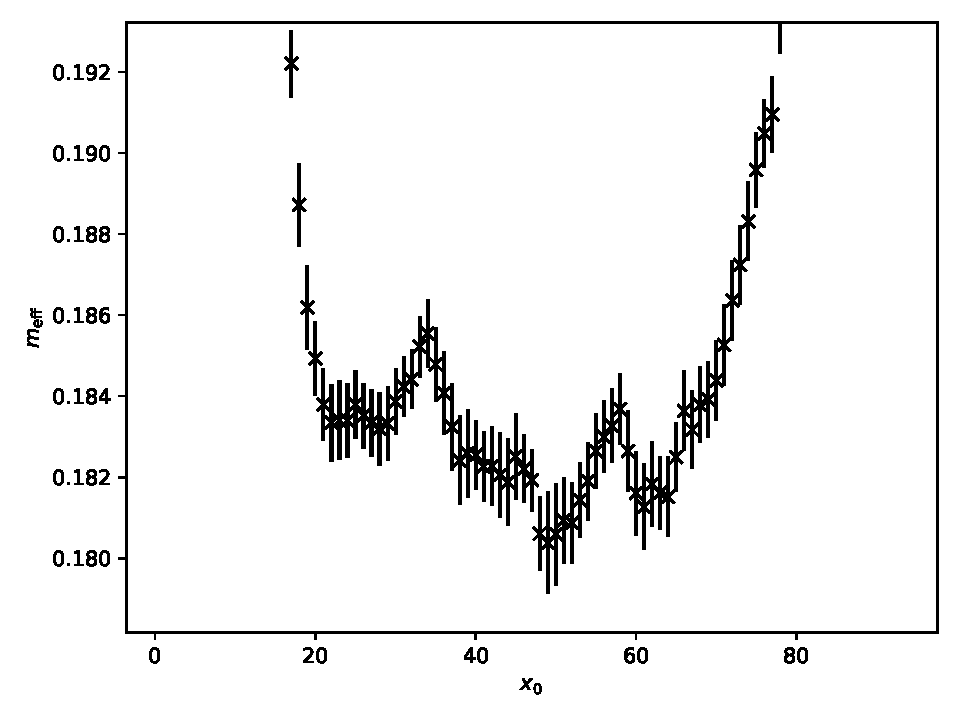
\includegraphics[width=\textwidth]{./cap3/figs/meff_H101.pdf}
    	\caption{}
    \end{subfigure}
    \begin{subfigure}{1.\textwidth}
    	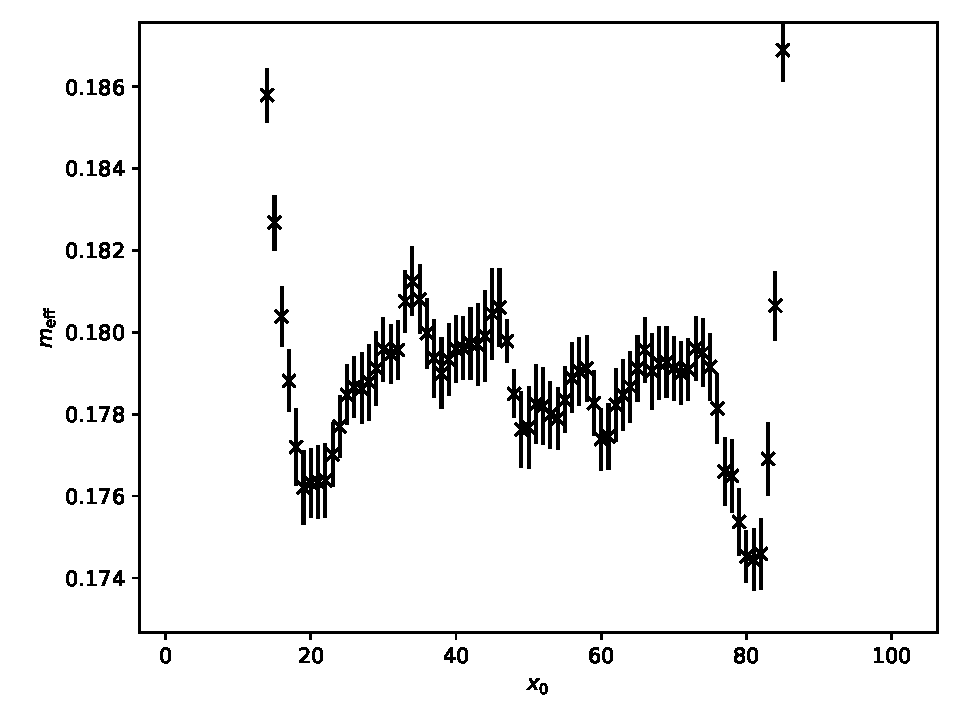
\includegraphics[width=\textwidth]{./cap3/figs/m_tm_H101.pdf}
    	\caption{}
    \end{subfigure}
    \caption{(a): pion effective mass $m_{\textrm{eff}}$ in eq.~(\ref{ch_observables:eq:meff}) for ensemble H101 in the Wilson regularization. (b): the same but for the mixed action regularization for one point in our valence parameters grid, see Sec.~\ref{ch_ma}.}
        \label{ch_observables:fig:meff}
\end{figure}

\begin{figure}
    \centering
    \begin{subfigure}{1.\textwidth}
    	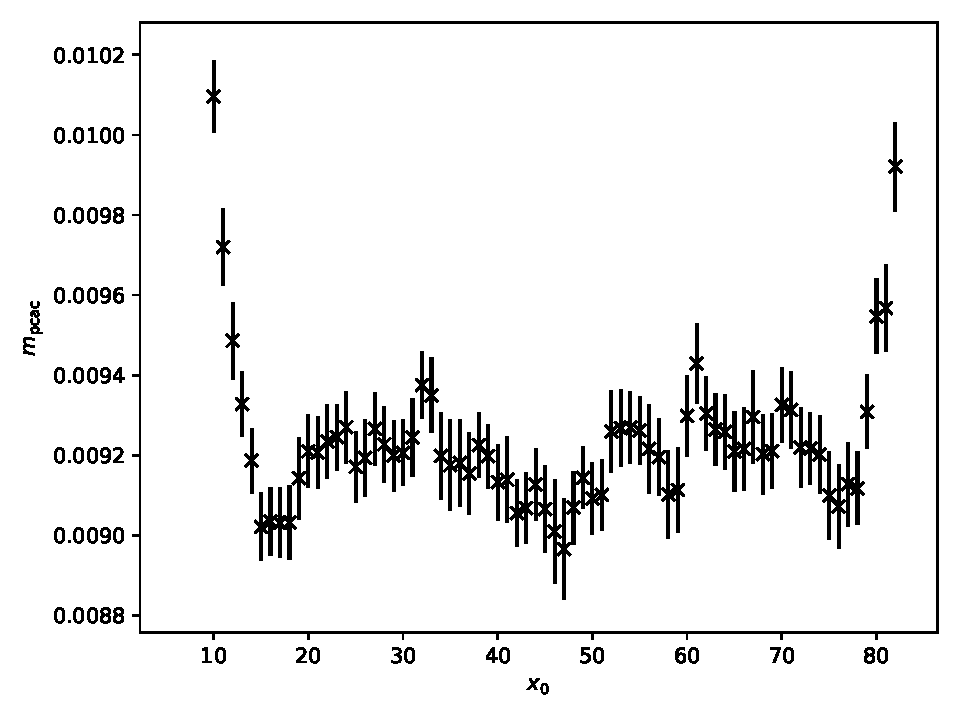
\includegraphics[width=\textwidth]{./cap3/figs/mpcac_H101.pdf}
    	\caption{}
    \end{subfigure}
    \begin{subfigure}{1.\textwidth}
    	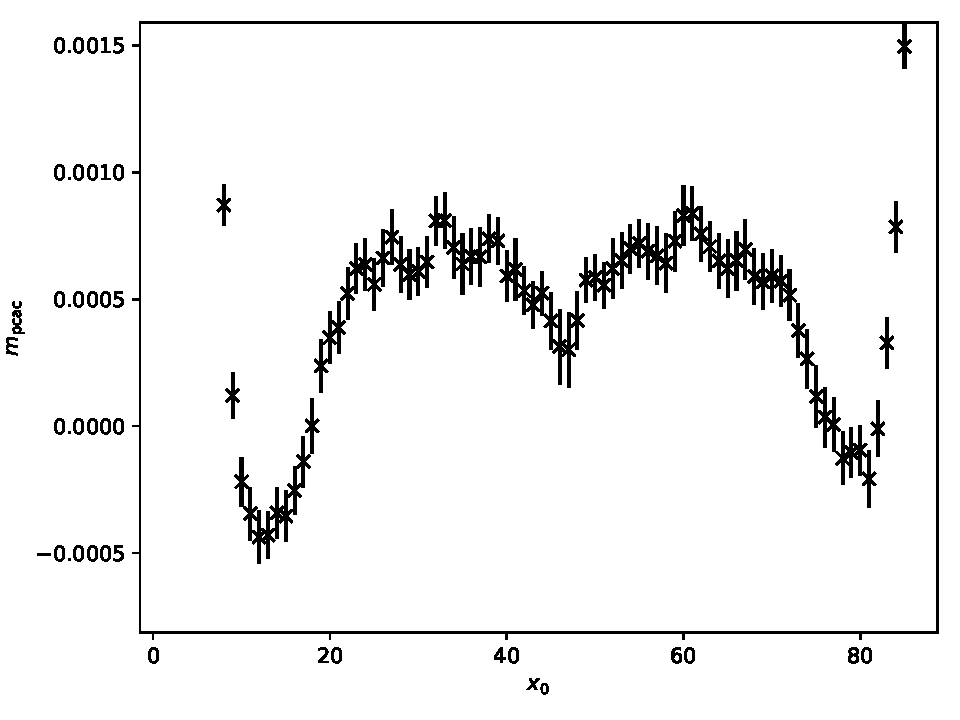
\includegraphics[width=\textwidth]{./cap3/figs/mpcac_tm_H101.pdf}
    	\caption{}
    \end{subfigure}
    \caption{(a): up/down PCAC quark mass in eq.~(\ref{ch_observables:eq:PCAC}) for ensemble H101 in the Wilson regularization. (b): the same but for the mixed action regularization for one point in our valence parameters grid, see Sec.~\ref{ch_ma}. At maximal twist this quantity must vanish.}
        \label{ch_observables:fig:mpcac}
\end{figure}

\begin{figure}
    \centering
    \begin{subfigure}{1.\textwidth}
    	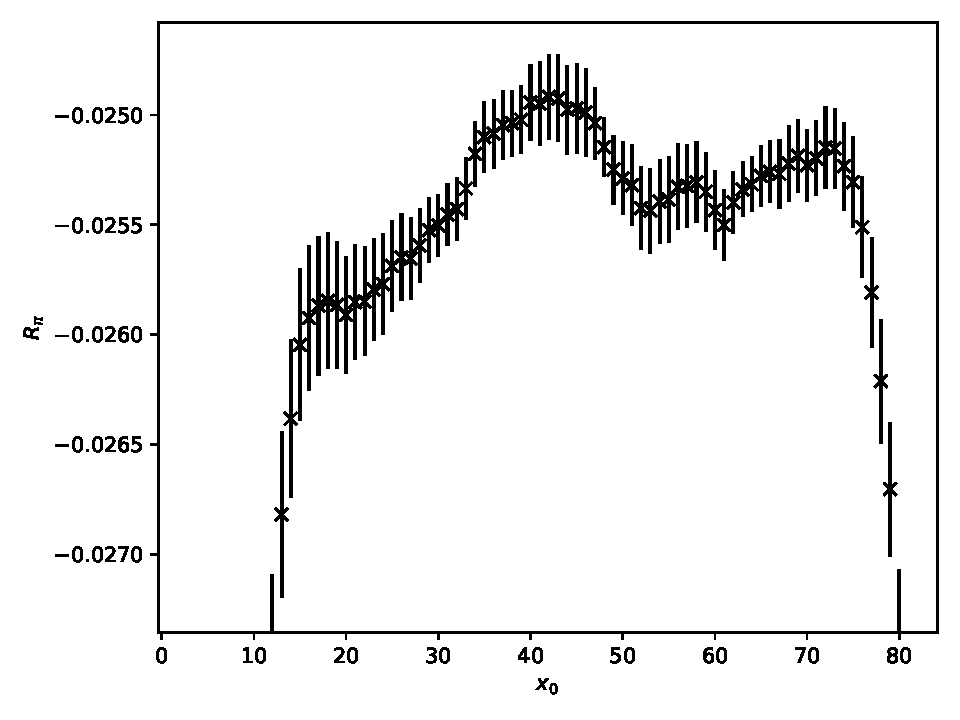
\includegraphics[width=\textwidth]{./cap3/figs/R_H101.pdf}
    	\caption{}
    \end{subfigure}
    \begin{subfigure}{1.\textwidth}
    	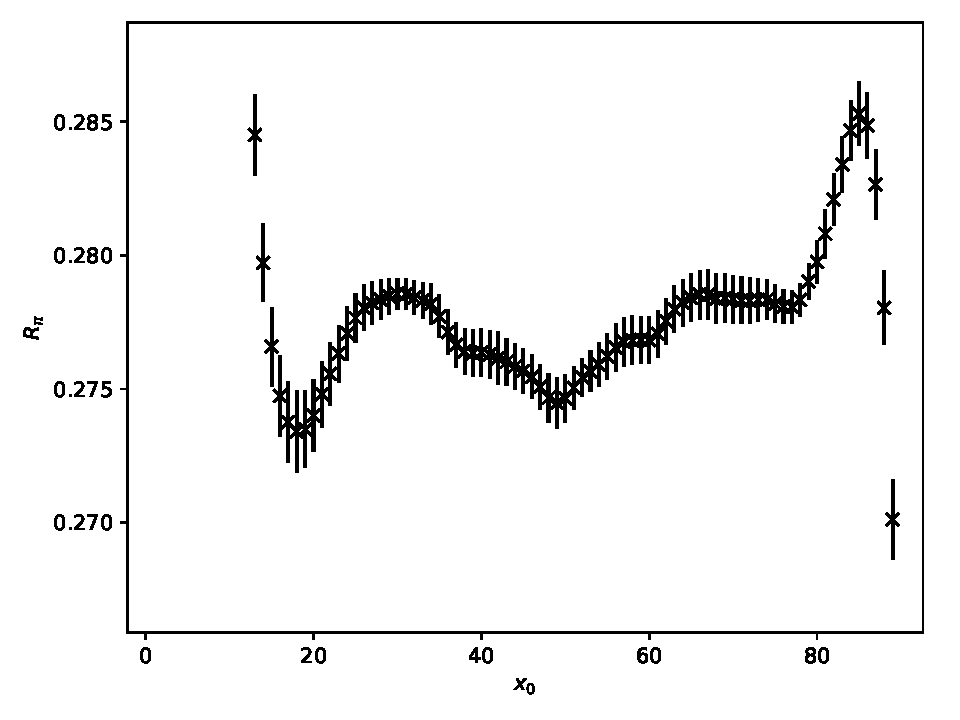
\includegraphics[width=\textwidth]{./cap3/figs/R_tm_H101.pdf}
    	\caption{}
    \end{subfigure}
    \caption{(a): vacuum-to-pion axial matrix element $R_{\pi}$ from eq.~(\ref{ch_observables:eq:R}) for ensemble H101 in the Wilson regularization. (b): vacuum-to-pion pseudoscalar matrix element $R_{\pi}$ from eq.~(\ref{ch_observables:eq:R_tm}) in the mixed action regularization for one point in our valence parameters grid, see Sec.~\ref{ch_ma}.}
        \label{ch_observables:fig:R}
\end{figure}

\begin{figure}
    \begin{subfigure}{1.\textwidth}
    	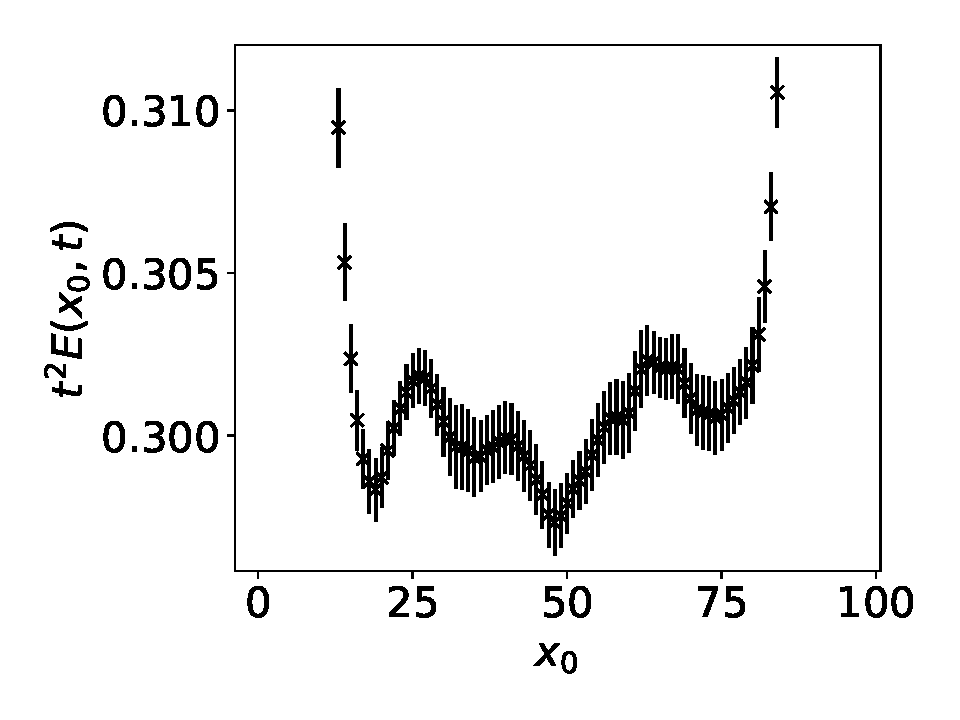
\includegraphics[width=\textwidth]{./cap3/figs/t2E_H101_plat.pdf}
    	\caption{}
    \end{subfigure}
    \begin{subfigure}{1.\textwidth}
    	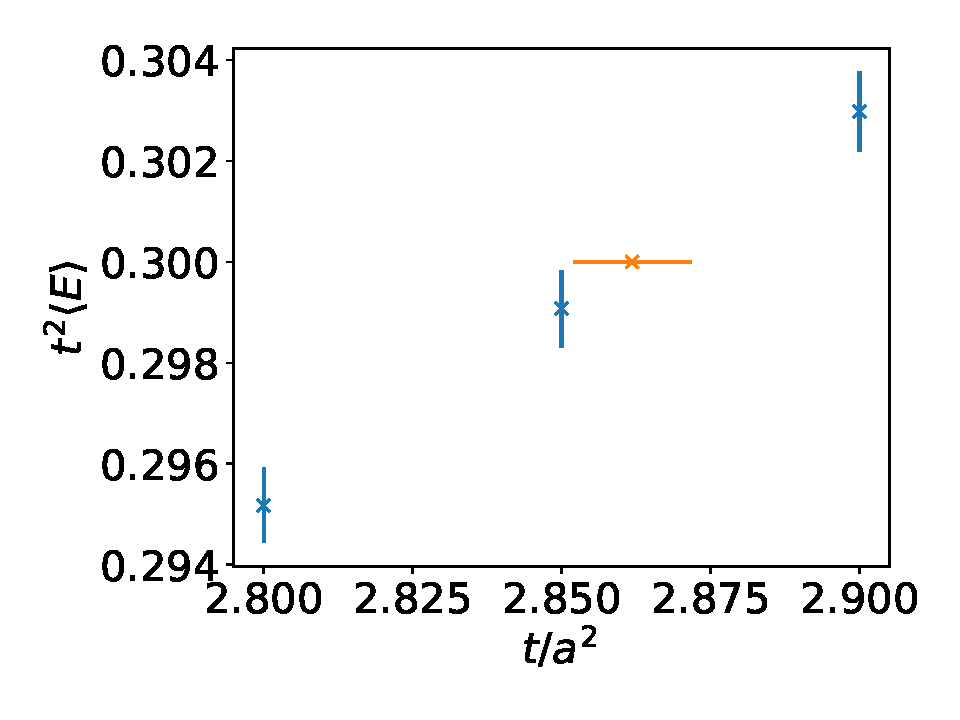
\includegraphics[width=\textwidth]{./cap3/figs/t0_H101.pdf}
    	\caption{}
    \end{subfigure}
    \caption{(a): $t^2E(x_0,t)$ for one value of the flow time $t/a^2$ near $t_0/a^2$ as a function of the Euclidean time $x_0/a$, with $E(x_0,t)$ the space volume averaged energy density. The latter is defined in eq.~(\ref{ch_observables:eq:E}). (b): Euclidean-time averaged values of $t^2\left<E(x_0,t)\right>_{x_0}$ for several flow times $t/a^2$ (blue points) near $t_0/a^2$ (defined in eq.~(\ref{ch_observables:eq:t0})) and the interpolated result for $t_0/a^2$ (orange point). Results for ensemble H101.}
        \label{ch_observables:fig:t2E}
\end{figure}

\begin{figure}
\centering
	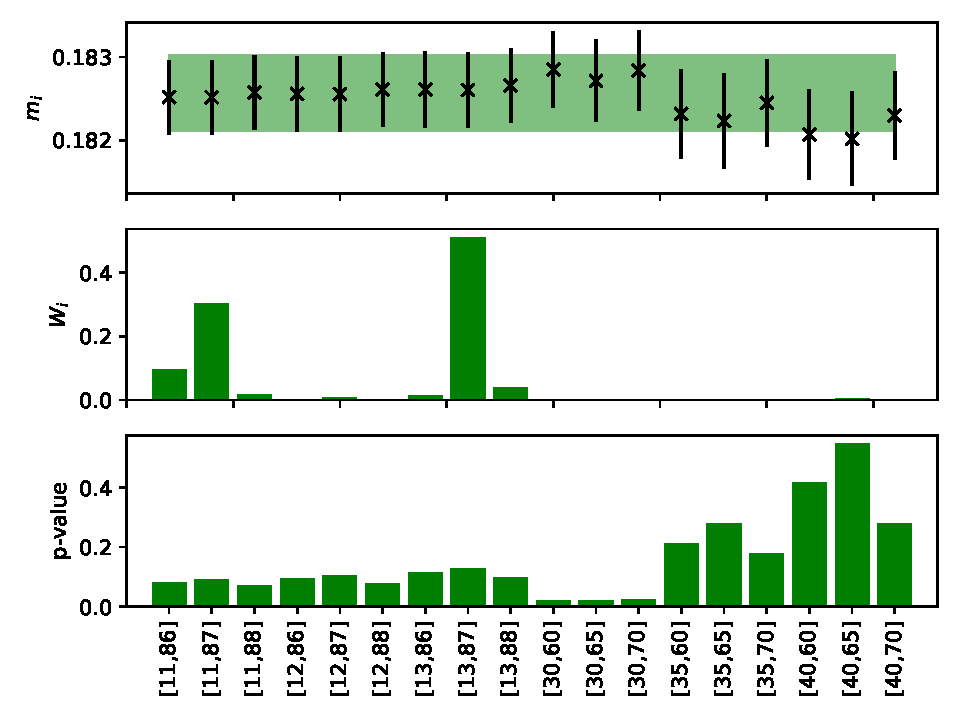
\includegraphics[width=1.\textwidth]{./cap3/figs/m_H101_pion_wil.pdf}
    \caption{Model variation for the extraction of the ground state signal of the pion effective mass of ensemble H101 in the Wilson regularization, shown in Fig.~\ref{ch_observables:fig:meff}. From top to bottom we show the ground state signal result from a fit to eq.~(\ref{ch_observables:eq:fit}) for each fit interval choice, the weight associated to each choice according to eq.~(\ref{ch_observables:eq:weight}), and the goodness of fit measured through the p-values defined in~\citep{Bruno:2022mfy}. We see that the highest weights are associated to a compromise between good fits (in terms of p-values) and fits with large number of points. The right-most models in the plot are heavily penalized even though they have the best p-values, since they cut a large number of points and models with not so severe cuts get also good p-values. The band in the top figure indicates the final weighted average result with the systematic uncertainty in eq.~(\ref{ch_observables:eq:syst}) included.}
    \label{ch_observables:fig:model_av}
\end{figure}



%%%%%%%%%%%%%%%%%%%%%%%%%%%%%%%%%%%%%%%%%%%%%%%%%%%%%%%%%%%
%%%%%%%%%%%%%%%%%%%%%%%%%%%%%%%%%%%%%%%%%%%%%%%%%%%%%%%%%%%

\cleardoublepage
\part{Precission Physics from a Lattice QCD Mixed Action}\label{pt:results}
\chapter{Mixed action setup}\addcontentsline{toc}{chapter}{Mixed action setup}

%%%%%%%%%%%%%%%%%%%%%%%%%%%%%%%%%%%%%%%%%%%%%%%%%%%%%%%%%%%
%%%%%%%%%%%%%%%%%%%%%%%%%%%%%%%%%%%%%%%%%%%%%%%%%%%%%%%%%%%
%%%%%%%%%%%%%%%%%%%%%%%%%%%%%%%%%%%%%%%%%%%%%%%%%%%%%%%%%%%
%%%%%%%%%%%%%%%%%%%%%%%%%%%%%%%%%%%%%%%%%%%%%%%%%%%%%%%%%%%

\label{ch_ma}

%%%%%%%%%%%%%%%%%%%%%%%%%%%%%%%%%%%%%%%%%%%%%%%%%%%%%%%%%%%
%%%%%%%%%%%%%%%%%%%%%%%%%%%%%%%%%%%%%%%%%%%%%%%%%%%%%%%%%%%
%%%%%%%%%%%%%%%%%%%%%%%%%%%%%%%%%%%%%%%%%%%%%%%%%%%%%%%%%%%
%%%%%%%%%%%%%%%%%%%%%%%%%%%%%%%%%%%%%%%%%%%%%%%%%%%%%%%%%%%

\section{Motivation}
\label{ch_ma:sec:introduction}

Our lattice setup is based on a mixed action with Wilson $\mathcal{O}(a)$ improved quarks in the sea and full twist Wilson tm quarks in the valence, the goal of which is to control cutoff effects associated with heavy quarks.

For the definition of the mixed action approach, we recall eq.~(\ref{ch_foundation:eq:path_int})
\begin{align}
\left<O^{ij}(x_1)O^{ji}(x_2)\right>&=-\frac{1}{\mathcal{Z}}\int\mathcal{D}[U]e^{-S_{\textrm{G}}[U]-S_{\textrm{eff}}[U]}\times\\&{\textrm{tr}}\left(\Gamma D_i^{-1}(x_1,x_2)\Gamma D_j^{-1}(x_2,x_1)\right),\\
S_{\textrm{eff}}[U]&=-\sum_i^{N_f}\textrm{log det}(D_i).
\end{align} 
We see that the Dirac operator $D$ appears first in the Boltzmann factor $e^{-S_{\textrm{G}}[U]-S_{\textrm{eff}}[U]}$ with which the set of gauge ensembles is generated, and then in the fermionic observable whose expectation value we are interested in. In particular, it appears in two separate stages of the analysis: one the generation of gauge ensembles, the other the inversion of the Dirac operator on said gauge configurations. This in principle allows for the use of different regularizations of the Dirac operator in these two steps, which is referred to as a mixed action approach.

The two separate sectors in which the Dirac operator appear, $S_{\textrm{eff}}$ and the observable whose expectation value one is interested in, are referred to as sea and valence sectors respectively. By using different lattice regularizations of the Dirac operator in both sectors, unitarity is violated, even in the continuum, if the physical quark masses in both sectors do not coincide. This means that our mixed action setup will require a tuning procedure in which the values of the Wilson tm parameters are chosen in order to reproduce the same physical quark masses in the valence as in the sea sectors. This process is called matching of the mixed action.

The flavor content of our setup is as follows. On the one hand, the sea sector has $N_f=2+1$ flavors, i.e. two mass-degenerate light quarks (corresponding to the $u$ and $d$ flavors) with mass $m_l$ and one strange quark with mass $m_s$. On the other hand, the valence sector is composed of $N_f=2+1+1$ flavors, adding a charm quark. Since we have $N_f=2+1$ in the sea and $N_f=2+1+1$ in the valence, the flavors we need to match are the light and strange, treating the charm quark in the valence as a partially quenched flavor. 

In order to perform the matching of the theory, we need to know beforehand what values the physical quark masses take in the sea sector. This means that we need lattice measurements in the fully Wilson unitary setup (using the Wilson regularization in the sea and valence) in addition to the mixed action regularization. We therefore have two sets of data for lattice observables: those coming from the Wilson unitary setup, which we refer to as sea or Wilson results, and those coming from the mixed action itself. Using the two sets of data helps increasing the statistics of the scale setting and light quark masses analysis, as we will see in Secs~\ref{ch_ss}-\ref{ch_qm}. In addition to the matching of the sea and valence sectors, we also need to tune the valence action parameters to enforce full twist and automatic $\mathcal{O}(a)$ improvement.

The Chapter is structured as follows. In Sec.~\ref{ch_ma:sec:Sea} we discuss the sea sector details: ensembles under study, lattice actions and boundary conditions. In Sec.~\ref{ch_ma:sec:Valence} we discuss the valence sector, which employs Wilson tm quarks. In Sec.~\ref{ch_ma:sec:chiral_traj} we discuss the line of constant physics along which the ensembles under study were generated. They follow a chiral trajectory that suffers small mistunings and that must be corrected in order to go through the physical point. We discuss the details of a mass shifting procedure to account for these effects. Finally, in Sec.~\ref{ch_ma:sec:matching} we deal with the challenges of working with a mixed action and the need to match both sea and valence sectors in order to recover unitarity in the continuum. We also explain the procedure to tune Wilson tm valence quarks to full twist.

%%%%%%%%%%%%%%%%%%%%%%%%%%%%%%%%%%%%%%%%%%%%%%%%%%%%%%%%%%%
%%%%%%%%%%%%%%%%%%%%%%%%%%%%%%%%%%%%%%%%%%%%%%%%%%%%%%%%%%%
%%%%%%%%%%%%%%%%%%%%%%%%%%%%%%%%%%%%%%%%%%%%%%%%%%%%%%%%%%%
%%%%%%%%%%%%%%%%%%%%%%%%%%%%%%%%%%%%%%%%%%%%%%%%%%%%%%%%%%%

\section{Sea sector}
\label{ch_ma:sec:Sea}

The gauge ensembles that we employ are CLS ensembles~\cite{CLS} with $N_f=2+1$ non-perturbatively $\mathcal{O}(a)$ improved Wilson fermions (see eq.~(\ref{ch_foundation:eq:DW_impr})). They use the Lüscher-Weisz gauge action~\cite{}, which has reduced $\mathcal{O}(a^2)$ effects and is defined in eqs.~(\ref{ch_foundation:eq:SG_impr}-\ref{ch_foundation:eq:LW}).

For most of the ensembles, open boundary conditions (OBC) in time are used for the gauge fields, since it has been shown that with periodic boundary conditions (PBC) autocorrelations increase as one approaches the continuum limit, a problem known as critical slowing down. This is related to the existence of topological disconnected sectors in gauge field space, which avoids the algorithm to sample correctly different topological sectors. In contrast to this, OBC let the topological charge flow through the boundaries and topology freezing is thus avoided. All ensembles use PBC over the spatial volume.

The ensembles we consider have 5 different values of the lattice spacing, and for each of them there is one ensemble at the symmetric point, which is defined as $m_l=m_s$, or equivalently by the $\kappa$ parameter (see eq.~(\ref{ch_foundation:eq:kappa})) as $\kappa_l=\kappa_s$. All the ensembles, the complete list of which is shown in Table~\ref{apex_ensembles:tab:ens}, follow the chiral trajectory defined in eq.~(\ref{ch_ma:eq:chiral_traj}).


%%%%%%%%%%%%%%%%%%%%%%%%%%%%%%%%%%%%%%%%%%%%%%%%%%%%%%%%%%%
%%%%%%%%%%%%%%%%%%%%%%%%%%%%%%%%%%%%%%%%%%%%%%%%%%%%%%%%%%%
%%%%%%%%%%%%%%%%%%%%%%%%%%%%%%%%%%%%%%%%%%%%%%%%%%%%%%%%%%%
%%%%%%%%%%%%%%%%%%%%%%%%%%%%%%%%%%%%%%%%%%%%%%%%%%%%%%%%%%%


\section{Valence sector}
\label{ch_ma:sec:Valence}

In the valence sector, we employ a $N_f=2+1+1$ fully-twisted Wilson tm fermion action (see Sec.~\ref{ch_foundation:subsec:tm}), whose Dirac operator reads
\begin{equation}
D_{\textrm{W}}+\boldsymbol{m}^{\textrm{(v)}}+i\boldsymbol{\mu}^{\textrm{(v)}}\gamma_5,
\end{equation}
with 
\begin{gather}
\boldsymbol{\mu}^{\textrm{(v)}}={\textrm{diag}}(\mu_l,-\mu_l,-\mu_s,\mu_c)^{\textrm{(v)}}, \quad
\boldsymbol{m}^{\textrm{(v)}}={\textrm{diag}}(m_l,m_l,m_s,m_c)^{\textrm{(v)}}.
\end{gather}
In particular, we use the same standard quark mass for all flavors $m_l^{\textrm{(v)}}=m_s^{\textrm{(v)}}=m_c^{\textrm{(v)}}\equiv m^{\textrm{(v)}}$.

As discussed in Sec.~\ref{ch_foundation:subsec:tm}, to impose full twist means that the twist angles $\alpha_i$ fulfill
\begin{equation}
{\textrm{cot}}\;\alpha_i=\frac{m_i^{\textrm{R}}}{\mu_i^{\textrm{R}}}=0.
\end{equation}
To do so, it is enough to impose that the PCAC quark masses in eq.~(\ref{ch_observables:eq:PCAC}) vanish. When this is the case, automatic $\mathcal{O}(a)$ improvement of valence observables is obtained, up to cutoff effects coming from the sea sector due to the mixed action. However, these effects are expected to be $\mathcal{O}(g_0^4)$ in perturbation theory.

Since we are dealing with a mixed action setup, not only the tuning to full twist is needed, but also a matching between the physical light and strange quark masses in the sea and valence sectors (see Sec.~\ref{ch_ma:sec:matching}) to ensure unitarity of the theory in the continuum limit. This means that we have to find the valence parameters $\left(\kappa,\mu_l,\mu_s\right)^{\textrm{(v)}}$ that satisfy both conditions. To do this, we employ a grid of valence values around an estimate of the target point in order to perform small interpolations that allow us to find the said target point $\left(\kappa,\mu_l,\mu_s\right)^{\textrm{(v)*}}$.

%%%%%%%%%%%%%%%%%%%%%%%%%%%%%%%%%%%%%%%%%%%%%%%%%%%%%%%%%%%
%%%%%%%%%%%%%%%%%%%%%%%%%%%%%%%%%%%%%%%%%%%%%%%%%%%%%%%%%%%
%%%%%%%%%%%%%%%%%%%%%%%%%%%%%%%%%%%%%%%%%%%%%%%%%%%%%%%%%%%
%%%%%%%%%%%%%%%%%%%%%%%%%%%%%%%%%%%%%%%%%%%%%%%%%%%%%%%%%%%

\section{Chiral trajectory}
\label{ch_ma:sec:chiral_traj}

The set of CLS ensembles that we use are generated along the trajectory in the quark mass plane defined by a constant trace of the bare sea ``(s)'' quark mass matrix
\begin{equation}
\label{ch_ma:eq:chiral_traj}
{\textrm{tr}}\left(M_q^{\textrm{(s)}}\right)=2m_l^{\textrm{(s)}}+m_s^{\textrm{(s)}}={\textrm{cnst}}.
\end{equation}
This trajectory ensures that at fixed lattice spacing the improved bare coupling 
\begin{equation}
\tilde{g}_0^2=g_0^2\left(1+b_g{\textrm{tr}}\left(aM_q^{\textrm{(s)}}\right)\right),
\end{equation}
is kept constant as we vary the sea quark masses to approach the physical point. Note that for the Wilson unitary setup, sea and valence quark masses are the same, but not for the mixed action setup. To ensure that this trajectory goes through the physical point, we define the dimensionless quantities
\begin{align}
\phi_2&=8t_0m_{\pi}^2,\\
\phi_4&=8t_0\left(m_K^2+\frac{1}{2}m_{\pi}^2\right),
\end{align}
which to LO ChPT are proportional to the renormalized quark masses
\begin{align}
\phi_2&\propto m_l^{\textrm{R}},\\
\phi_4&\propto2m_l^{\textrm{R}}+m_s^{\textrm{R}}={\textrm{tr}}\left(M_q^{\textrm{R}}\right).
\end{align}
The trace of the renormalized quark mass matrix ${\textrm{tr}}\left(M_q^{\textrm{R}}\right)$ is in turn proportional to the bare quark mass matrix up to $\mathcal{O}(a)$ cutoff effects
\begin{equation}
{\textrm{tr}}\left(M_q^{\textrm{R}}\right)=Z_mr_m\left[\left(1+a\bar{d}_m{\textrm{tr}}\left(M_q\right)\right){\textrm{tr}}\left(M_q\right)+ad_m{\textrm{tr}}\left(M_q^2\right)\right].
\end{equation}
Thus, setting the sea value of $\phi_4$ to its physical value for all ensembles ensure that eq.~(\ref{ch_ma:eq:chiral_traj}) holds and goes through the physical point, up to small mistunings due to higher terms in the chiral expansion and to cutoff effects. 

To correct for these mistunings, we perform small mass shifts~\cite{BKS} in the bare sea quark masses by Taylor expanding lattice observables as
\begin{equation}
\label{ch_ma:eq:mass_shift}
\mathcal{O}\left(m_l^{\textrm{(s)'}},m_s^{\textrm{(s)'}}\right)=\mathcal{O}\left(m_l^{\textrm{(s)}},m_s^{\textrm{(s)}}\right)+\sum_q\left(m_q^{\textrm{(s)'}}-m_q^{\textrm{(s)}}\right)\frac{d\mathcal{O}}{dm_q^{\textrm{(s)}}},
\end{equation}
with the total derivative given by
\begin{equation}
\label{ch_ma:eq:md}
\frac{d\mathcal{O}}{dm_q^{\textrm{(s)}}}=\sum_i\frac{\partial\mathcal{O}}{\partial \left<P_i\right>}\left[\left<\frac{\partial P_i}{\partial m_q^{\textrm{(s)}}}\right>-\left<P_i\frac{\partial S}{\partial m_q^{\textrm{(s)}}}\right>+\left<P_i\right>\left<\frac{\partial S}{\partial m_q^{\textrm{(s)}}}\right>\right].
\end{equation}
Here $\mathcal{O}$ is an arbitrary lattice observable and $\{P_i\}_{i=1,2,...}$ is the set of primary observables, in our case the corresponding two-point functions on which it depends. The first term in the r.h.s. of this equation corresponds to the valence contribution to the derivative, while the other terms correspond to the sea contributions. Note that for the Wilson unitary setup, all terms contribute, while for the mixed action setup, since the two-point functions $\{P_i\}$ do not depend explicitly on $m_q^{\textrm{(s)}}$, the first term in the r.h.s. of eq.~(\ref{ch_ma:eq:md}) vanishes.

In particular the sum over $q$ in eq.~(\ref{ch_ma:eq:mass_shift}) can be done in any direction of the quark mass plane, and we choose to mass shift only the strange quark. For practical purposes, since we want to mass shift all relevant observables for each ensemble to satisfy that the sea value of $\phi_4$ is equal to its physical value, $\phi_4^{\textrm{(s)}}=\phi_4^{\textrm{ph}}={\textrm{const.}}$, we rewrite the Taylor expansion as
\begin{equation}
\mathcal{O}\left(\phi_4^{\textrm{(s)'}}=\phi_4^{\textrm{ph}}\right)=\mathcal{O}\left(\phi_4^{\textrm{(s)}}\right)+\left(\phi_4^{\textrm{ph}}-\phi_4^{\textrm{(s)}}\right)\frac{d\mathcal{O}}{d\phi_4^{\textrm{(s)}}},
\end{equation}
with
\begin{equation}
\frac{d\mathcal{O}}{d\phi_4^{\textrm{(s)}}}=\frac{d\mathcal{O}/dm_s^{\textrm{(s)}}}{d\phi_4^{\textrm{(s)}}/dm_s^{\textrm{(s)}}}.
\end{equation}
Note that by sea value $\phi_4^{\textrm{(s)}}$ we refer to $\phi_4$ computed in the Wilson unitary setup, and its derivative has both sea and valence contributions, while $d\mathcal{O}/dm_s^{\textrm{(s)}}$ has valence and sea contributions when the observable $\mathcal{O}$ is computed in the Wilson unitary setup, and only sea contributions when $\mathcal{O}$ is computed in the mixed action regularization. In the Wilson unitary setup, imposing $\phi_4^{\textrm{(s)}}=\phi_4^{\textrm{ph}}={\textrm{const.}}$ means that so does the valence value of $\phi_4$, while for the mixed action regularization this is not true. In this case in addition to fixing $\phi_4^{\textrm{(s)}}=\phi_4^{\textrm{ph}}={\textrm{const.}}$ with the mass shifting procedure we need later to impose $\phi_4^{\textrm{(v)}}=\phi_4^{\textrm{(s)}}$, which is done through the matching between sea and valence sectors.

The observables we will be interested for the scale setting (see Sec.~\ref{ch_ss}) are $\sqrt{t_0}f_{\pi}$, $\sqrt{t_0}f_{K}$ and $\sqrt{t_0}f_{\pi K}$, the latter defined in eq.~(\ref{ch_ss:eq:fpik}), while for the determination of the physical quark masses (see Sec.~\ref{ch_qm}) we need $\sqrt{t_0}m_{12}^{\textrm{R}}$, $\sqrt{t_0}m_{13}^{\textrm{R}}$. All these quantities are physical and so are their derivatives w.r.t. $\phi_4$. Thus, one can measure these derivatives for each ensemble and then fit them as a function of $\phi_2$ and the lattice spacing. This allows to evaluate the result of these fits at the values of $\phi_2$ and $t_0/a^2$ corresponding to each ensemble and perform the mass shift with that result instead of using the individual measurements of each ensemble. This has the advantage of improving the precision for observables whose mass derivatives are noisy (or even not computed), which is particularly relevant for the finest lattice spacing and the most chiral ensembles under study.

For fitting the derivatives we use
\begin{equation}
\label{ch_ma:eq:md_1}
F=A+B\phi_2+D\frac{a^2}{t_0},
\end{equation}
for all choices of $\mathcal{O}$ except for the PCAC quark masses, for which we use
\begin{equation}
\label{ch_ma:eq:md_2}
F=A+B\phi_2+C\phi_2^2+(D+E\phi_2)\frac{a^2}{t_0},
\end{equation}
for empirical reasons.

In the case of $\phi_2$ in the Wilson regularization, we exclude the symmetric point ensembles from the fit of its mass derivative, since $\phi_2^{\textrm{sym}}=\frac{2}{3}\phi_4$ by construction. Thus, for these ensembles we will use this relation directly to mass shift $\phi_2$.

Results for the fit parameters are presented in Table~\ref{ch_ma:tab:md}, while plots are shown in Figs.~\ref{ch_ma:fig:d_w}-\ref{ch_ma:fig:d_tm}.

We have assumed knowledge of the physical value of $\phi_4$ to which we mass shift all ensembles. However, in order to determine it we need the physical value of the intermediate scale $t_0$, which is the target of the analysis. Thus, we start the process with an educated guess of $t_0^{\textrm{ph}}$, which provides with an initial guess for $\phi_4^{\textrm{ph}}$. Once the scale setting has been done and a new determination of $t_0^{\textrm{ph}}$ is obtained, the analysis is iterated, updating the value of $\phi_4^{\textrm{ph}}$ to which the ensembles are shifted, until convergence is observed in this observable. The initial guess used for $t_0^{\textrm{ph,\;guess}}$ is just a number with no error. After several iterative steps of the analysis, we obtain the new estimate
\begin{equation}
\label{ch_ma:eq:t0_guess}
t_0^{\textrm{ph,\;guess}}=0.1445(6),
\end{equation}
where the uncertainty keeps all the correlations with the lattice data entering the analysis. Eq.~(\ref{ch_ma:eq:t0_guess}) determines the value of $\phi_4^{\textrm{ph}}$ to which we perform the mass shifts in the subsequent sections, the input values for $m_{\pi}$ and $m_K$ given in eq.~(\ref{ch_ss:eq:isoQCD}). 

\begin{longtable}{c | c c c c c}
\label{ch_ma:tab:md}
    $\mathcal{O}$ & A & B & C & D & E \\
    \toprule
    $\sqrt{t_0}f_{\pi K}^{\textrm{W}}$ & 0.017(8) & -0.007(10) & - & 0.024(26) & - \\ 
    $\sqrt{t_0}f_{\pi}^{\textrm{W}}$ & 0.006(8) & 0.008(9) & - & 0.020(26) & - \\ 
    $\sqrt{t_0}f_{K}^{\textrm{W}}$ & 0.024(10) & -0.016(11) & - & 0.022(27) & - \\ 
    $\sqrt{t_0}m_{12}^{\textrm{W, R}}$ & 0.006(4) & -0.033(13) & 0.090(12) & 0.046(17) & -0.074(27) \\ 
    $\sqrt{t_0}m_{13}^{\textrm{W, R}}$ & 0.050(6) & 0.030(17) & -0.066(18) & -0.069(33) & 0.070(45) \\ 
    $\phi_2^{\textrm{W}}$ & 0.004(36) & 0.131(92) & - & 0.874(129) & - \\ 
    $t_0$ & -0.437(84) & 0.214(101) & - & -0.264(274) & - \\ 
    \midrule
    $\sqrt{t_0}f_{\pi K}^{\textrm{tm}}$ & -0.009(7) & 0.011(8) & - & -0.014(18) & - \\ 
    $\sqrt{t_0}f_{\pi}^{\textrm{tm}}$ & -0.007(6) & 0.013(8) & - & -0.028(18) & - \\ 
    $\sqrt{t_0}f_{K}^{\textrm{tm}}$ & -0.009(8) & 0.010(10) & - & -0.006(18) & - \\ 
    $\sqrt{t_0}m_{12}^{\textrm{tm, R}}$ & -0.004(3) & 0.035(10) & -0.041(9) & 0.020(16) & 0.026(24) \\ 
    $\phi_2^{\textrm{tm}}$ & 0.031(17) & -0.032(23) & - & -0.102(73) & - \\ 
    $\phi_4^{\textrm{tm}}$ & 0.006(37) & 0.050(47) & - & -0.298(126) & - \\ 
    \bottomrule
    \caption{Results for the fit parameters in eqs.~(\ref{ch_ma:eq:md_1}-\ref{ch_ma:eq:md_2}) for the lattice observables that will be used in the analysis. The superscript ``W'' refers to the observable being computed in the Wilson unitary setup, while ``tm'' refers to the mixed action setup.}
\end{longtable}

\begin{figure}
    \centering
    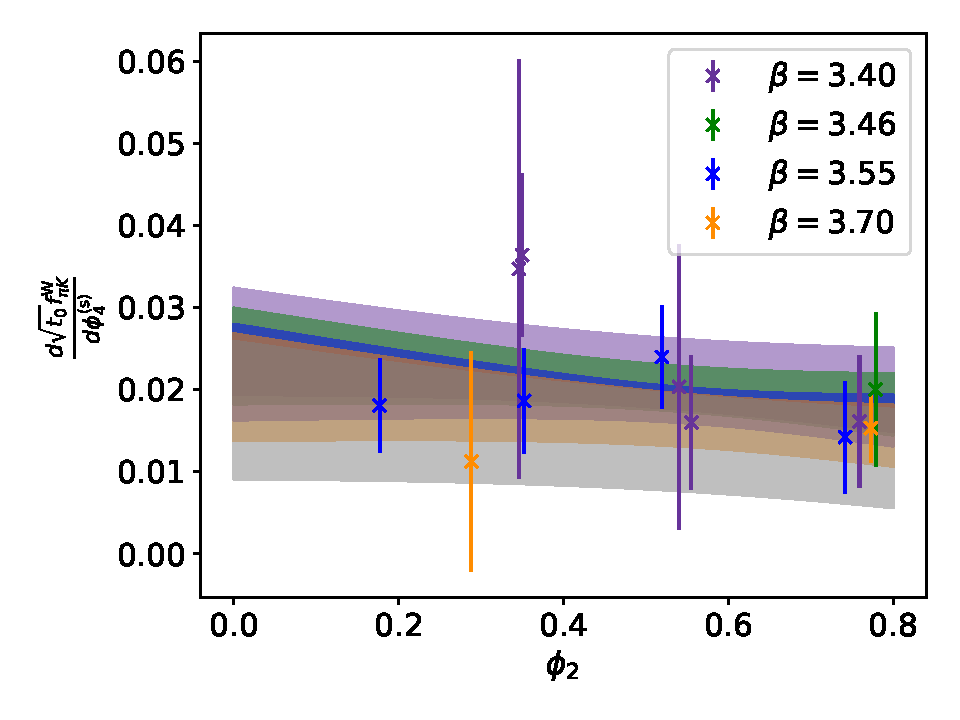
\includegraphics[width=.49\textwidth]{./cap4/figs/dt0fpik_w.pdf}
    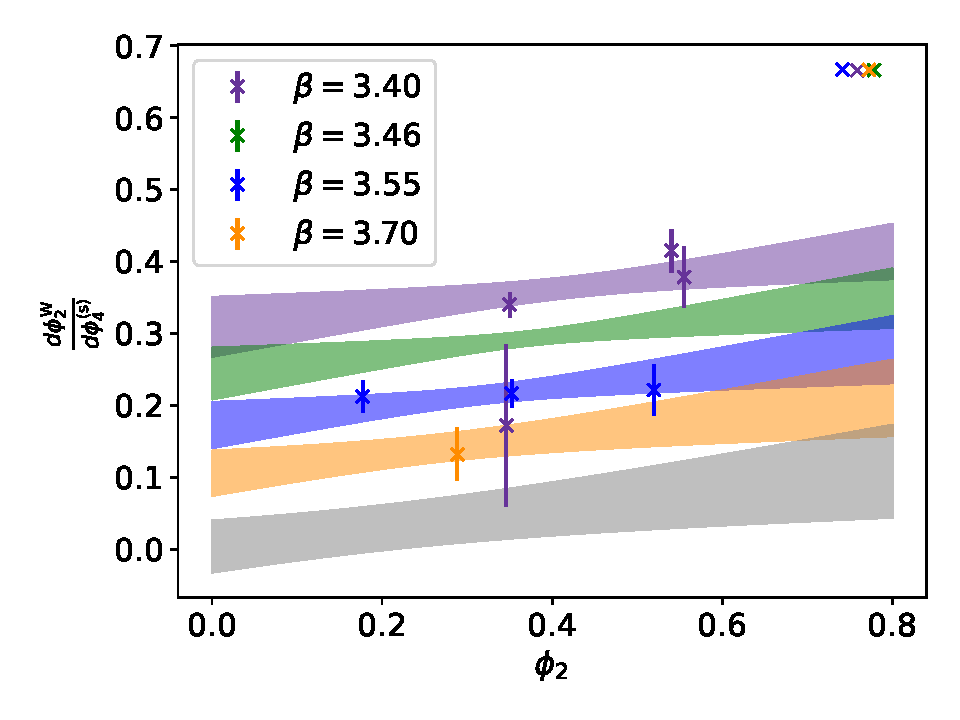
\includegraphics[width=.49\textwidth]{./cap4/figs/dphi2_w.pdf}
    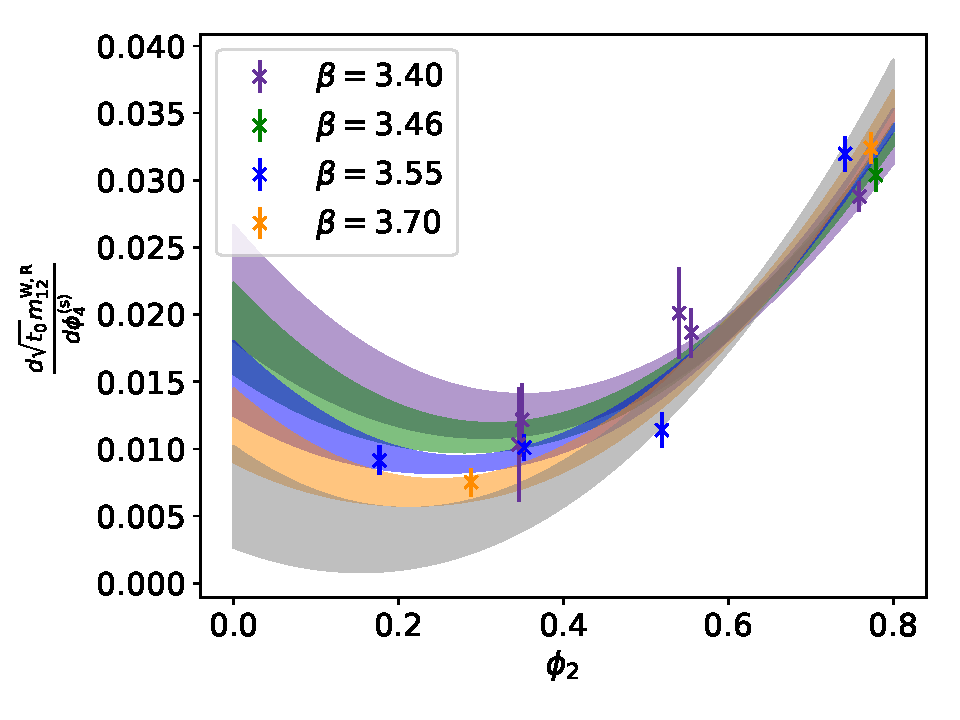
\includegraphics[width=.49\textwidth]{./cap4/figs/dt0m12_w.pdf}
    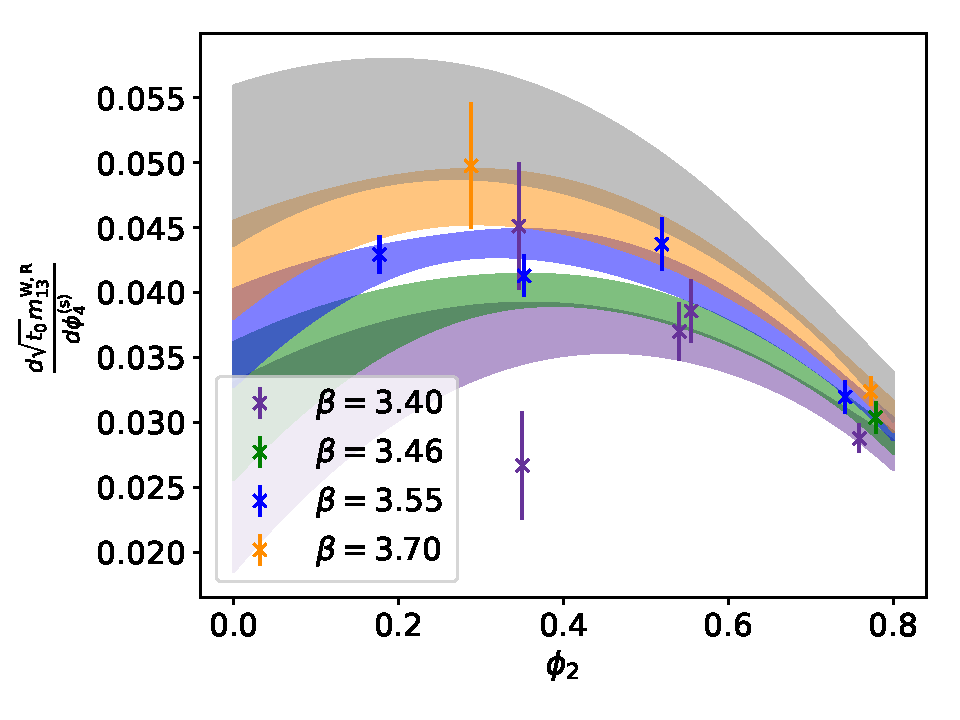
\includegraphics[width=.49\textwidth]{./cap4/figs/dt0m13_w.pdf}
    \caption{Derivatives $dO/d\phi_4^{\textrm{(s)}}$ for the Wilson unitary setup for $O=\sqrt{t_0}f_{\pi K},\;\phi_2,\;\sqrt{t_0}m_{12}^{\textrm{R}},\;\sqrt{t_0}m_{13}^{\textrm{R}}$. For the fit eqs.~(\ref{ch_ma:eq:md_1}-\ref{ch_ma:eq:md_2}) were used. Results for the fit parameters are presented in Table~\ref{ch_ma:tab:md}.}
    \label{ch_ma:fig:d_w}
\end{figure}

\begin{figure}
    \centering
    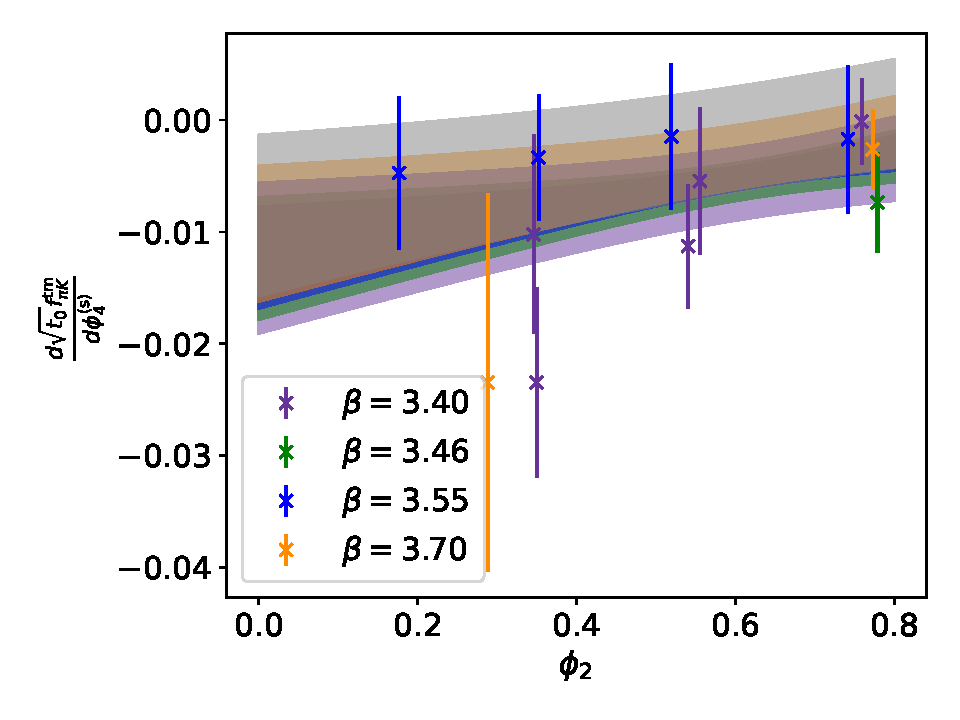
\includegraphics[width=.49\textwidth]{./cap4/figs/dt0fpik_tm.pdf}
    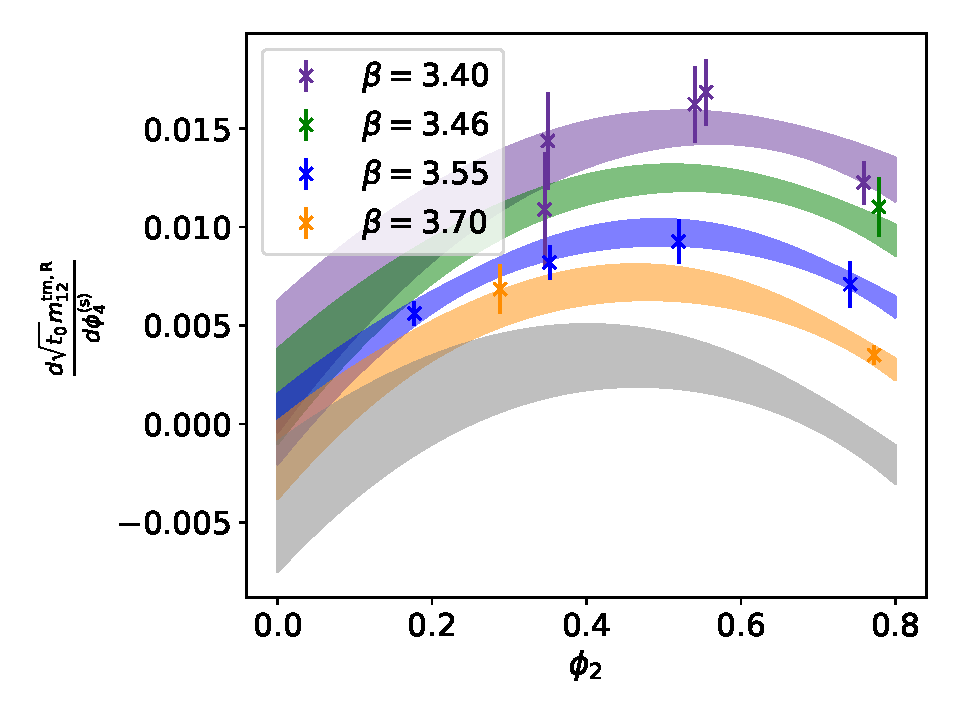
\includegraphics[width=.49\textwidth]{./cap4/figs/dt0m12_tm.pdf}
    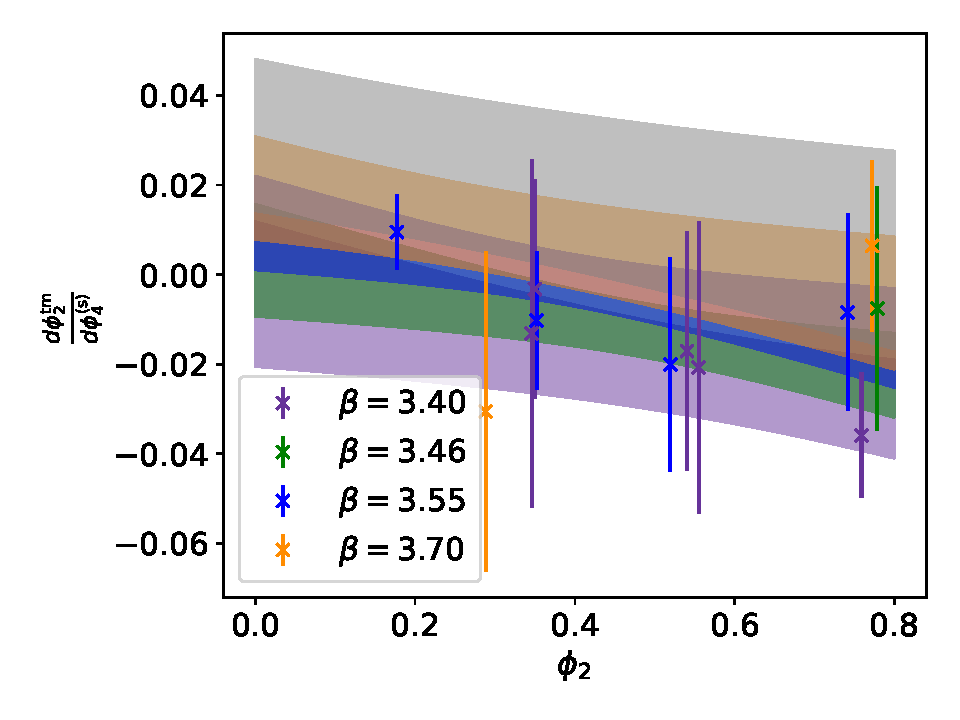
\includegraphics[width=.49\textwidth]{./cap4/figs/dphi2_tm.pdf}
    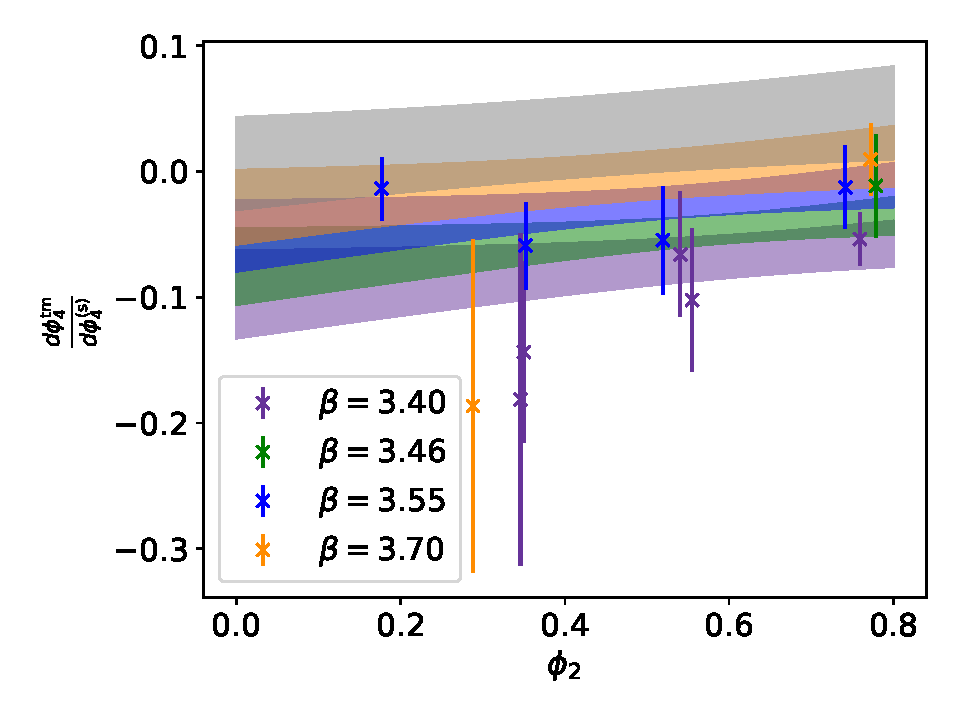
\includegraphics[width=.49\textwidth]{./cap4/figs/dphi4_tm.pdf}
    \caption{Derivatives $dO/d\phi_4^{\textrm{(s)}}$ for the mixed action setup for $O=\sqrt{t_0}f_{\pi K},\;\phi_2,\;\phi_4,\;\sqrt{t_0}m_{12}^{\textrm{R}}$. For the fit eqs.~(\ref{ch_ma:eq:md_1}-\ref{ch_ma:eq:md_2}) were used. Results for the fit parameters are presented in Table~\ref{ch_ma:tab:md}.}
    \label{ch_ma:fig:d_tm}
\end{figure}

%%%%%%%%%%%%%%%%%%%%%%%%%%%%%%%%%%%%%%%%%%%%%%%%%%%%%%%%%%%
%%%%%%%%%%%%%%%%%%%%%%%%%%%%%%%%%%%%%%%%%%%%%%%%%%%%%%%%%%%
%%%%%%%%%%%%%%%%%%%%%%%%%%%%%%%%%%%%%%%%%%%%%%%%%%%%%%%%%%%
%%%%%%%%%%%%%%%%%%%%%%%%%%%%%%%%%%%%%%%%%%%%%%%%%%%%%%%%%%%


\section{Matching and tuning at full twist}
\label{ch_ma:sec:matching}

As explained in Sec.~\ref{ch_ma:sec:Valence}, when working with a mixed action, after performing the mass shifts in section.~\ref{ch_ma:sec:chiral_traj}, we need to match the physical quark masses of the sea and valence sectors. To do this, we use a grid of valence parameter values to find the target point with small interpolations. In order to know the values of the relevant observables in the sea, we need measurements in the fully Wilson unitary setup (with Wilson fermions in both sea and valence). These will be referred to as Wilson or sea data or results, while the mixed action measurements, once the matching is done, will be referred to as Wtm or mixed action data or results.

In practice, to compute the physical quark masses we need the relevant improvement coefficients. In order not to rely on these for the matching procedure, instead of matching the physical quark masses $m_l^{\textrm{R}},\;m_s^{\textrm{R}}$, we choose to use the pion and kaon masses in units of the gradient flow scale $t_0$
\begin{align}
\label{ch_ma:eq:matching}
\phi_2^{\textrm{(s)}}&=\phi_2^{\textrm{(v)}},\\
\phi_4^{\textrm{(s)}}&=\phi_4^{\textrm{(v)}}.
\end{align}
since these quantities are proportional to the physical quark masses to LO ChPT.

In addition to this, we need to tune the Wilson tm action to full twist, which means setting the PCAC quark mass to zero
\begin{equation}
\label{ch_ma:eq:full-twist}
m_{ud}^{\textrm{(v)}}=m_{ll'}^{\textrm{(v)}}\equiv m_{12}^{\textrm{(v)}}=0.
\end{equation}
In principle, we should also send the strange PCAC quark mass to zero. However, since the $\kappa^{\textrm{(v)}}$ parameter we use is flavor degenerate, this condition is automatically satisfied (up to cutoff effects, see Fig.~\ref{}) once eq.~(\ref{ch_ma:eq:full-twist}) is imposed.

To impose eqs.~(\ref{ch_ma:eq:matching}-\ref{ch_ma:eq:full-twist}), we perform interpolations of the valence observables $m_{12}^{\textrm{(v)}},\phi_2^{\textrm{(v)}},\phi_4^{\textrm{(v)}}$ in the $\left(\kappa,\mu_l,\mu_s\right)^{\textrm{(v)}}$ hyperplane, using as fit functions the following expressions motivated by ChPT
\begin{align}
m_{12}^{\textrm{(v)}}&=p_1\left(\frac{1}{\kappa^{\textrm{(v)}}}-\frac{1}{\kappa^{\textrm{(v)*}}}\right)+p_2\left(\mu_l^{\textrm{(v)}}-\mu_l^{\textrm{(v)*}}\right),\\
\phi_2^{\textrm{(v)}}&=\frac{p_3}{\mu_l^{\textrm{(v)}}}\left(\frac{1}{\kappa^{\textrm{(v)}}}-\frac{1}{\kappa^{\textrm{(v)*}}}\right)^2+p_4\left(\mu_l^{\textrm{(v)}}-\mu_l^{\textrm{(v)*}}\right)+\phi_2^{\textrm{(s)}},\\
\phi_2^{\textrm{(v)}}&=\frac{p_5}{\mu_l^{\textrm{(v)}}}\left(\frac{1}{\kappa^{\textrm{(v)}}}-\frac{1}{\kappa^{\textrm{(v)*}}}\right)^2+\frac{p_6}{\mu_s^{\textrm{(v)}}}\left(\frac{1}{\kappa^{\textrm{(v)}}}-\frac{1}{\kappa^{\textrm{(v)*}}}\right)^2 \\
&+p_7\left(\mu_l^{\textrm{(v)}}-\mu_l^{\textrm{(v)*}}\right)+p_8\left(\mu_s^{\textrm{(v)}}-\mu_s^{\textrm{(v)*}}\right)+\phi_4^{\textrm{(s)}}.
\end{align}
This way, the target point values $\left(\kappa,\mu_l,\mu_s\right)^{\textrm{(v)*}}$ are found as fit parameters. The interpolation is shown in Fig.~\ref{ch_ma:fig:match}. A simultaneous fit of these three quantities is performed.

The mixed action results for the quark masses are given exactly by the target twist mass parameters $\mu_{l,s}^{\textrm{(v)*}}$, while the extraction of the pion and kaon decay constants in the mixed action setup requires a new interpolation along the valence grid to the target point. The fit functions for this interpolation are
\begin{align}
f_{\pi}^{\textrm{(v)}}&=q_1\left(\frac{1}{\kappa^{\textrm{(v)}}}-\frac{1}{\kappa^{\textrm{(v)*}}}\right)^2+q_2\left(\frac{1}{\kappa^{\textrm{(v)}}}-\frac{1}{\kappa^{\textrm{(v)*}}}\right)+q_3\mu_l^{\textrm{(v)}},\\
f_K^{\textrm{(v)}}&=r_1\left(\frac{1}{\kappa^{\textrm{(v)}}}-\frac{1}{\kappa^{\textrm{(v)*}}}\right)^2+r_2\left(\frac{1}{\kappa^{\textrm{(v)}}}-\frac{1}{\kappa^{\textrm{(v)*}}}\right)+r_3\mu_l^{\textrm{(v)}}+r_4\mu_s^{\textrm{(v)}}.
\end{align}
The interpolation for the decay constants combination $f_{\pi K}$ defined in eq.~(\ref{ch_ss:eq:fpik}) is shown in Fig.~\ref{ch_ma:fig:fpik_interp}.

\begin{figure}
    \centering
    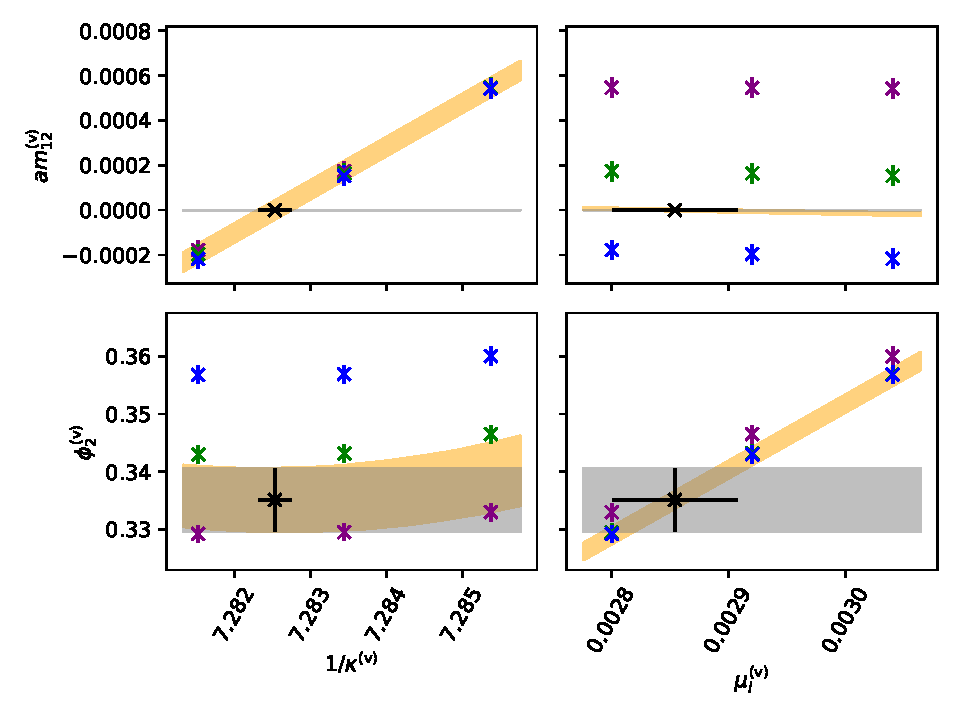
\includegraphics[width=1.\textwidth]{./cap4/figs/matching_H105.pdf}
    \caption{Plot of the matching of sea (gray band) and valence values of $\phi_2$ and tune to full twist $am_{12}^{\textrm{(v)}}=0$ along the grid of valence parameters values. Each point represents a different measurement of a lattice observables in the valence along the grid, and the orange band represents the interpolation. The black point is the target result $\left(\kappa,\mu_l,\mu_s\right)^{\textrm{(v)*}}$. Here we only show the matching of $\phi_2^{\textrm{(v)}}$ and $am_{12}^{\textrm{(v)}}$, though the matching of $\phi_4^{\textrm{(v)}}$ is done simultaneously. Ensemble is H105.}
    \label{ch_ma:fig:match}
\end{figure}

\begin{figure}
    \centering
    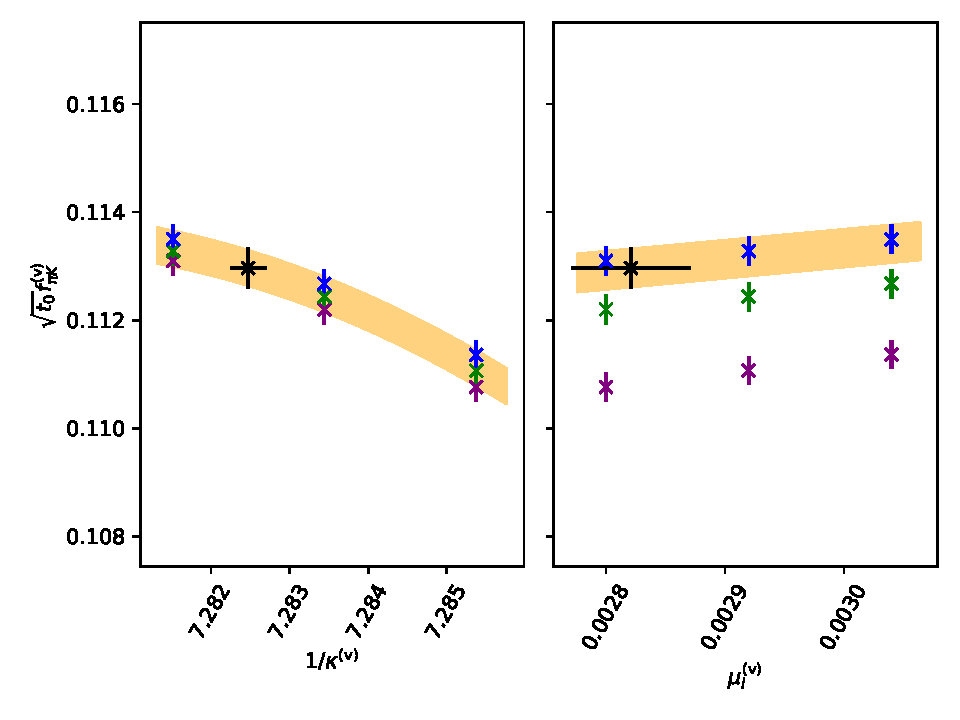
\includegraphics[width=1.\textwidth]{./cap4/figs/interp_fpik_H105.pdf}
    \caption{Interpolation of $\sqrt{t_0}f_{\pi K}$ (see eq.~(\ref{ch_ss:eq:fpik})) along the valence grid to the target point $\left(\kappa,\mu_l,\mu_s\right)^{\textrm{(v)*}}$. The points with different colors represent measurements at different values of the valence parameters. Ensemble is H105.}
    \label{ch_ma:fig:fpik_interp}
\end{figure}

%%%%%%%%%%%%%%%%%%%%%%%%%%%%%%%%%%%%%%%%%%%%%%%%%%%%%%%%%%%
%%%%%%%%%%%%%%%%%%%%%%%%%%%%%%%%%%%%%%%%%%%%%%%%%%%%%%%%%%%
%%%%%%%%%%%%%%%%%%%%%%%%%%%%%%%%%%%%%%%%%%%%%%%%%%%%%%%%%%%
%%%%%%%%%%%%%%%%%%%%%%%%%%%%%%%%%%%%%%%%%%%%%%%%%%%%%%%%%%%

\chapter{Scale setting}\addcontentsline{toc}{chapter}{Scale setting}

%%%%%%%%%%%%%%%%%%%%%%%%%%%%%%%%%%%%%%%%%%%%%%%%%%%%%%%%%%%
%%%%%%%%%%%%%%%%%%%%%%%%%%%%%%%%%%%%%%%%%%%%%%%%%%%%%%%%%%%
%%%%%%%%%%%%%%%%%%%%%%%%%%%%%%%%%%%%%%%%%%%%%%%%%%%%%%%%%%%
%%%%%%%%%%%%%%%%%%%%%%%%%%%%%%%%%%%%%%%%%%%%%%%%%%%%%%%%%%%

\label{ch_ss}

%%%%%%%%%%%%%%%%%%%%%%%%%%%%%%%%%%%%%%%%%%%%%%%%%%%%%%%%%%%
%%%%%%%%%%%%%%%%%%%%%%%%%%%%%%%%%%%%%%%%%%%%%%%%%%%%%%%%%%%
%%%%%%%%%%%%%%%%%%%%%%%%%%%%%%%%%%%%%%%%%%%%%%%%%%%%%%%%%%%
%%%%%%%%%%%%%%%%%%%%%%%%%%%%%%%%%%%%%%%%%%%%%%%%%%%%%%%%%%%

\section{Motivation}
\label{ch_ss:sec:introduction}

The scale setting involves the precise determination of one reference observable, the scale, in physical units, to which any other observable is compared in order to extract the value of the latter in physical units. 

We decide to use the gradient flow scale $t_0$ introduced in Sec.~\ref{ch_observables:sec:Flow} as an intermediate reference scale since it can be computed in the lattice with high precision. Following the discussion in Sec.~\ref{ch_foundation:sec:ss}, we choose for the phenomenological input the decay constants of the pion and kaon
\begin{equation}
\label{ch_ss:eq:fpik}
\Lambda\equiv f_{\pi K}=\frac{2}{3}\left(f_K+\frac{1}{2}f_{\pi}\right).
\end{equation}
After measuring $\sqrt{t_0}f_{\pi K}$ for each ensemble, one must perform a chiral-continuum limit in order to extract its value at the physical point and in the continuum. To define the physical point we use the pion and kaon masses, or equivalently the dimensionless quantities $\phi_2$ and $\phi_4$. For the determination of the physical value of these quantities we need again the physical value of $t_0$, which is the target of the analysis. As in Sec.~\ref{ch_ma}, we start with an initial guess in eq.~(\ref{ch_ma:eq:t0_guess}) and iterate the analysis until convergence is observed. Thus, with each iterative step both the values of $\phi_2$ to which we perform the chiral extrapolation and the value of $\phi_4$ to which we shifted our observables are updated. 

Since all lattice observables and the action that we use are $\mathcal{O}(a)$ improved, we expect lattice artifacts to start at $\mathcal{O}(a^2)$. In order to perform the chiral-continuum limit, we explore different ways of parameterizing the dependence on $\phi_2,\;\phi_4$ and on the lattice spacing $a$, and employ the same techniques of model averaging discussed in Sec.~\ref{ch_observables:sec:MA}.

After performing the chiral-continuum limit, using as external physical input the values of the pion and kaon decay constants we can determine the value of the scale $t_0$ as
\begin{equation}
\sqrt{t_0^{\textrm{ph}}}=\frac{\left.\begin{matrix}
\left(\sqrt{t_0}f_{\pi K}\right)^{\textrm{latt}}
\end{matrix}\right|_{a=0}}{f_{\pi K}^{\textrm{exp}}}.
\end{equation}

In particular, we are studying ensembles which employ $N_f=2+1$ fermions, and thus assume isospin symmetry for the light flavor. This means that the physical input for the masses and decay constants we need is not that of Nature, but that of isosymmetric QCD (isoQCD). These values are given by the Flavor Lattice Average Group (FLAG) in~\cite{FLAG21}
\begin{gather}
\label{ch_ss:eq:isoQCD}
m_{\pi}^{\textrm{isoQCD}}=134.9768(5)\;{\textrm{MeV}}, \quad
m_{K}^{\textrm{isoQCD}}=497.611(13)\;{\textrm{MeV}}, \\
f_{\pi}^{\textrm{isoQCD}}=130.56(2)_{\textrm{exp}}(13)_{\textrm{QED}}(2)_{|V_{ud}|}\;{\textrm{MeV}}, \quad \\
f_{K}^{\textrm{isoQCD}}=157.2(2)_{\textrm{exp}}(2)_{\textrm{QED}}(4)_{|V_{us}|}\;{\textrm{MeV}}.
\end{gather} 
As we see, the kaon decay constant receives a large contribution to its uncertainty from the determination of the $|V_{us}|$ CKM matrix element. Also, QED corrections are stronger in the kaon than in the pion. All these subtleties motivate a scale setting that uses only the pion decay constant as physical input. For this reason we also study this possibility when doing the model variation for the chiral-continuum extrapolation.

%%%%%%%%%%%%%%%%%%%%%%%%%%%%%%%%%%%%%%%%%%%%%%%%%%%%%%%%%%%
%%%%%%%%%%%%%%%%%%%%%%%%%%%%%%%%%%%%%%%%%%%%%%%%%%%%%%%%%%%
%%%%%%%%%%%%%%%%%%%%%%%%%%%%%%%%%%%%%%%%%%%%%%%%%%%%%%%%%%%
%%%%%%%%%%%%%%%%%%%%%%%%%%%%%%%%%%%%%%%%%%%%%%%%%%%%%%%%%%%


\section{Results: the physical point}
\label{ch_ss:sec:Results}

The choice of the decay constants to set the scale, and in particular of the combination in eq.~(\ref{ch_ss:eq:fpik}) is due to its chiral behavior, since at fixed value of $\phi_4$ (as in our case thanks to the mass shifting procedure, see Sec.~\ref{ch_ma:sec:chiral_traj}) to NLO SU(3) ChPT it only depends on $\phi_2$ through chiral logarithms, 
\begin{align}
\label{ch_ss:eq:SU3ChPT}
&F_{\chi,\pi K}^{\textrm{cont}}(\phi_2)\equiv\left(\sqrt{8t_0}f_{\pi K}\right)^{\textrm{cont}}=\\
&=\frac{A}{4\pi}\left[1+\frac{7}{6}L\left(\frac{\phi_2}{A^2}\right)-\frac{4}{3}L\left(\frac{\phi_4-\frac{1}{2}\phi_2}{A^2}\right)-\frac{1}{2}L\left(\frac{\frac{4}{3}\phi_4-\phi_2}{A^2}\right)+B\phi_4\right],
\end{align}
with the chiral logarithms given by
\begin{equation}
\label{ch_ss:eq:log}
L(x)=x{\textrm{log}}\left(x\right),
\end{equation}
and $A,B$ related to chiral low energy constants (LEC). We use this expression to perform the chiral-continuum extrapolation of $\sqrt{t_0}f_{\pi K}$. We will use the label $[SU(3)\chi PT]$ for this continuum dependence. 

Another possibility for the physical point extrapolation is to use Taylor expansions in $\phi_2$ around the symmetric point. We can either go to second or fourth order in the Taylor expansion
\begin{equation}
\label{ch_ss:eq:Tay}
F_{\textrm{Tay},\pi K}^{\textrm{cont}}(\phi_2)\equiv\sqrt{8t_0}f_{\pi K}^{\textrm{cont}}=A+B\left(\phi_2-\phi_2^{\textrm{sym}}\right)^2,
\end{equation}
or
\begin{equation}
\label{ch_ss:eq:Tay4}
F_{\textrm{Tay},\pi K}^{\textrm{cont}}(\phi_2)=A+B\left(\phi_2-\phi_2^{\textrm{sym}}\right)^2+C\left(\phi_2-\phi_2^{\textrm{sym}}\right)^4,
\end{equation}
labeling these models as $[Tay]$ and $[Tay4]$. Due to symmetry reasons, there are no terms with odd powers of $\phi_2$~\cite{}.

Since the kaon decay constant is expected to receive more severe QED corrections than the pion, and the determination of its physical value for isosymmetric-QCD is affected by the uncertainty of the element of the CKM matrix $|V_{us}|$, we can also use the quantity $\sqrt{t_0}f_{\pi}$ to set the scale, and SU(2) ChPT to perform the physical point extrapolation. According to the latter,
\begin{align}
F_{\chi,\pi}^{\textrm{cont}}(\phi_2)\equiv\sqrt{8t_0}f_{\pi}^{\textrm{cont}}&=A\phi_2+B\left(1-2L\left(\frac{\phi_2}{B^2}\right)\right),\\
F_{\chi,K}^{\textrm{cont}}(\phi_2)\equiv\sqrt{8t_0}f_K^{\textrm{cont}}&=C\phi_2+D\left(1-\frac{3}{4}L\left(\frac{\phi_2}{B^2}\right)\right),
\end{align}
in which case we fit both $f_{\pi}$ and $f_K$ since they share a fit parameter, in order to help control the extrapolation in $f_{\pi}$. In the end, however, we set the scale only with external input for $f_{\pi}$.

In addition to the extrapolation in the pion mass, we need to supplement these fit functions with cutoff effects in order to describe our lattice data. For this we will explore two possibilities
\begin{align}
\label{ch_ss:eq:a2}
F^{\textrm{latt}}(\phi_2)&=F^{\textrm{cont}}(\phi_2)+W\frac{a^2}{8t_0},\\
F^{\textrm{latt}}(\phi_2)&=F^{\textrm{cont}}(\phi_2)+W\frac{a^2}{8t_0}\alpha_S^{\Gamma_1},\\
F^{\textrm{latt}}(\phi_2)&=F^{\textrm{cont}}(\phi_2)+\left(W+Z\phi_2\right)\frac{a^2}{8t_0}.
\end{align}
We assign the labels $[a^2]$, $[a^2\alpha_S^{\Gamma}]$ and $[a^2+a^2\phi_2]$ to characterize the lattice artifacts of these models.

In order to assess the systematic uncertainty in the extraction of $\sqrt{t_0}$, we will explore all these continuum-chiral extrapolations and their different results. In the same direction we also explore the impact of performing data cuts from the fits. In particular, we consider the following cuts (in addition to the ``no cut'' choice)
\begin{gather}
\beta>3.40, \quad
\beta>3.46, \quad
\phi_2<0.6, \\
\phi_2<0.4, \quad
\beta>3.40\;\&\;\phi_2<0.6, \\
m_{\pi}L>4.1.
\end{gather}

Finally, to perform all of these fits, we have two data sets: the Wilson unitary setup and the mixed action. Both must share the same continuum limit, but different cutoff effects. We can thus perform the continuum-chiral extrapolations for the Wilson data, for the mixed action, or for a combined data set, parameterizing the data with the same continuum limit behavior $F^{\textrm{cont}}(\phi_2)$ but different cutoff effects (different $W,Z$ fit parameters for Wilson and mixed action data). This third choice allows to further constrain the continuum extrapolation and keep it well under control, while increasing the statistics and getting better precision for $\sqrt{t_0}$. As a universality check, we perform the continuum limit of only symmetric point ensembles of both the Wilson and mixed action data, without imposing a common value in the continuum. Since all these points have the same $\phi_2$ they follow a line of constant physics as we approach the continuum. This extrapolation is shown in Fig.~\ref{ch_ss:fig:universality} and indeed it shows that both data sets agree perfectly well in the continuum, with the mixed action data having much milder cutoff effects.

Once the various models to extrapolate to the continuum and physical point have been explored, we use the model averaging technique in Sec.~\ref{ch_observables:sec:MA} to assign a weight to each model 
\begin{equation}
\label{ch_ss:eq:W}
W\propto\exp\left(-\frac{1}{2}\left(\chi^2-2\left<\chi^2\right>\right)\right),
\end{equation}
that allows us to compute a weighted average for $\sqrt{t_0}$, as well as the associated systematic uncertainty
\begin{align}
\left<\sqrt{t_0}\right>&=\sum_i\sqrt{t_0^{(i)}}W^{(i)},\\
\sigma^2_{\textrm{syst}}&=\left<\sqrt{t_0}^2\right>-\left<\sqrt{t_0}\right>^2.
\end{align}

In Figs.~\ref{ch_ss:fig:BMA_w}-\ref{ch_ss:fig:BMA_comb} we show the model average results for the Wilson unitary setup, for the mixed action and for the combined analysis. In Appendix~\ref{apex_model_av_t0} we show the numerical results of $\sqrt{t_0}$ for each model considered, together with their weights and p-values, for the Wilson, mixed action and combined analysis. In Fig.~\ref{ch_ss:fig:SU3a2} we show the pion mass dependence of the continuum-chiral extrapolation for one of the best models explored in terms of the TIC for the combined data sets, together with the lattice spacing dependence for the same model, projecting all points to the physical pion mass $\phi_2^{\textrm{ph}}$ using the fit result for the continuum piece $F^{\textrm{cont}}(\phi_2)$.

The final results for $\sqrt{t_0}$ in physical units as computed from the model average for the different data sets are
\begin{align}
\label{ch_ss:eq:t0ph}
\sqrt{t_0}&=0.1436(7)_{\textrm{stat}}(3)_{\textrm{syst}}\;\textrm{fm, Wilson}, \\
\sqrt{t_0}&=0.1441(9)_{\textrm{stat}}(6)_{\textrm{syst}}\;\textrm{fm, Mixed action}, \\
\sqrt{t_0}&=0.1440(6)_{\textrm{stat}}(4)_{\textrm{syst}}\;\textrm{fm, Combined}.
\end{align}

\begin{figure}
    \centering
    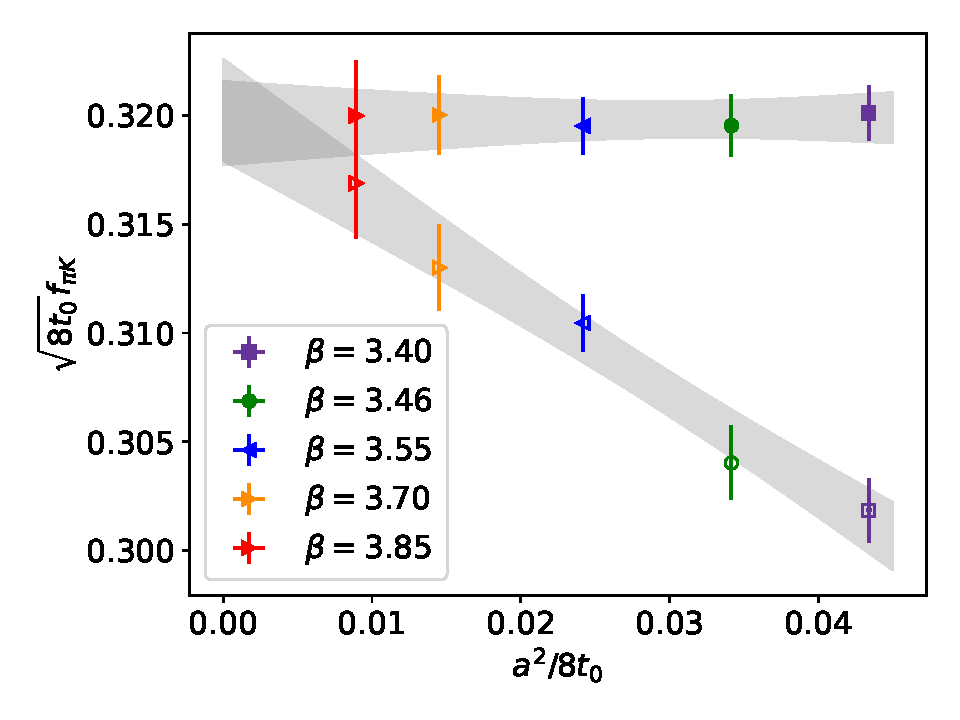
\includegraphics[width=.7\textwidth]{./cap5/figs/continuum_sym.pdf}
    \caption{Continuum limit of symmetric point ensembles for the Wilson unitary results or sea data set (empty points) and for the mixed action results (filled points). A common continuum limit is not imposed. Cutoff effects are parameterized as pure $\mathcal{O}(a^2)$ artifacts.}
    \label{ch_ss:fig:universality}
\end{figure}

\begin{figure}
    \centering
    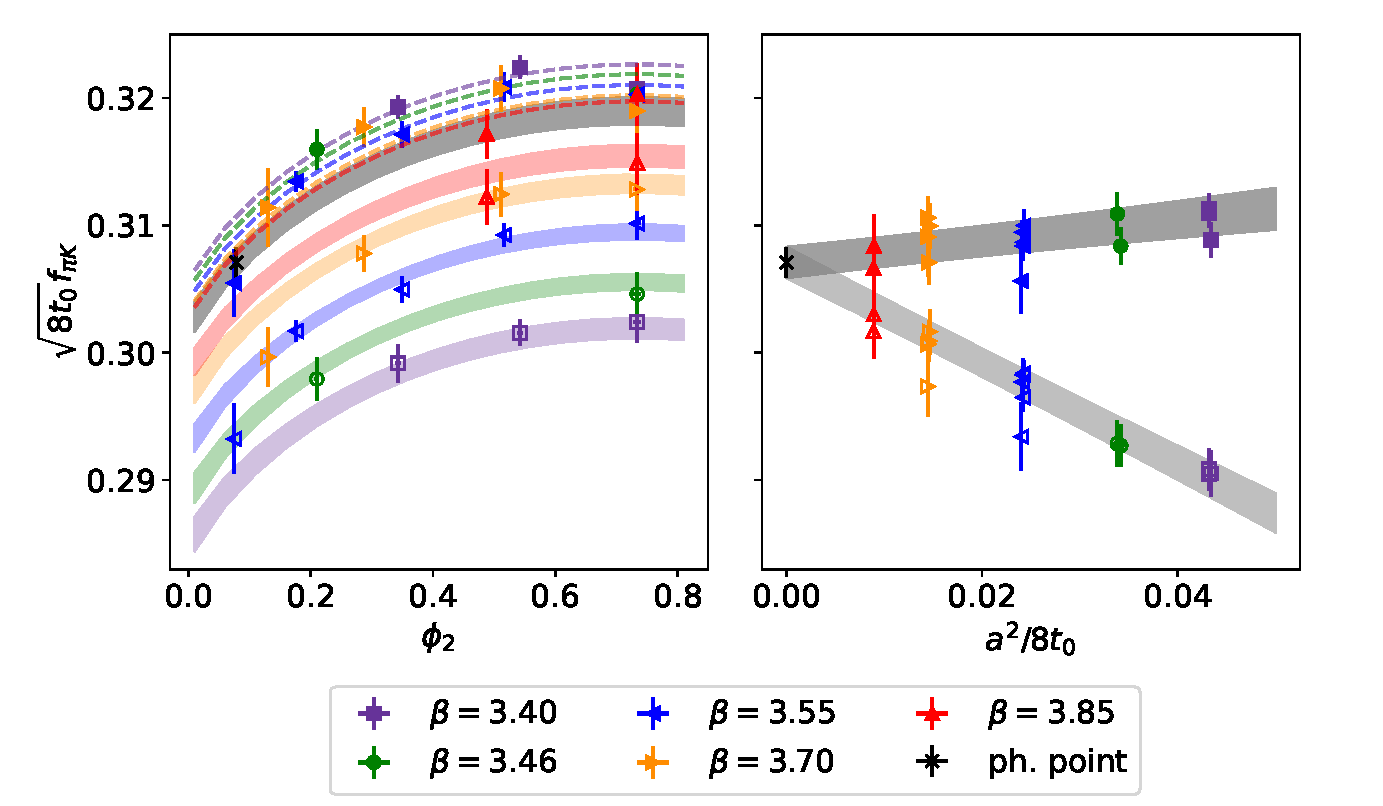
\includegraphics[width=1.\textwidth]{./cap5/figs/SU3_comb.pdf}
    \caption{\textit{Left}: Pion mass dependence of $\sqrt{8t_0}f_{\pi K}$ for the SU(3) ChPT model with pure $\mathcal{O}(a^2)$ cutoff effects: $[SU(3)\chi PT][a^2][-]$. We show the result of the combined fit of both Wilson (empty) and mixed action (filled) results. The colored bands represent the pion mass dependence for each lattice spacing for the Wilson results, while the dashed lines represent the dependence for the mixed action results. In the latter case we only plot the central value of the corresponding bands for visualization purposes. \textit{Right}: the same model, with point projected to the physical pion mass $\phi_2^{\textrm{ph}}$ using the fit result for the continuum mass dependence $F(\phi_2)^{\textrm{cont}}$. In this plot we show the lattice spacing dependence of our ensembles. We show two physical point results: the rightmost in the plot corresponds to the result coming from the fit model itself, while the leftmost is the result obtained from the model average.}
    \label{ch_ss:fig:SU3a2}
\end{figure}

\begin{figure}
    \centering
    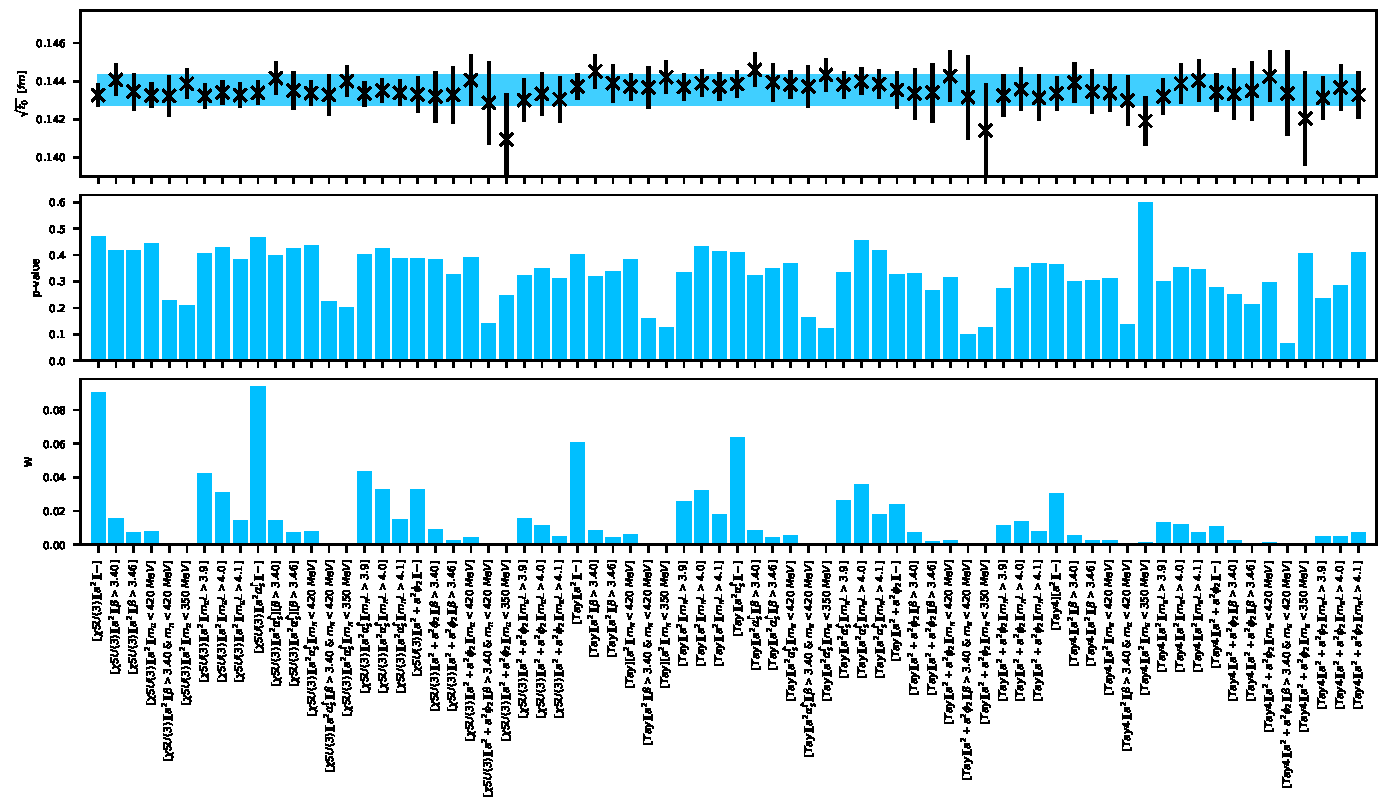
\includegraphics[width=1.\textwidth]{./cap5/figs/BMA_w.pdf}
    \caption{Model average results for the determination of $\sqrt{t_0}$ at the physical point using the Wilson results. In the top figure we show the results coming from each fit model together with the final averaged result with the systematic uncertainty coming from the model variation added (blue band). In the middle plot we show the quality of fits as measured by the p-value~\cite{chi_exp}. In the bottom figure we show the assigned weight to each model according to eq.~(\ref{ch_ss:eq:W}). We provide a Table connecting each label to the corresponding fit models in Appendix~\ref{apex_model_av_t0}.}
    \label{ch_ss:fig:BMA_w}
\end{figure}

\begin{figure}
    \centering
    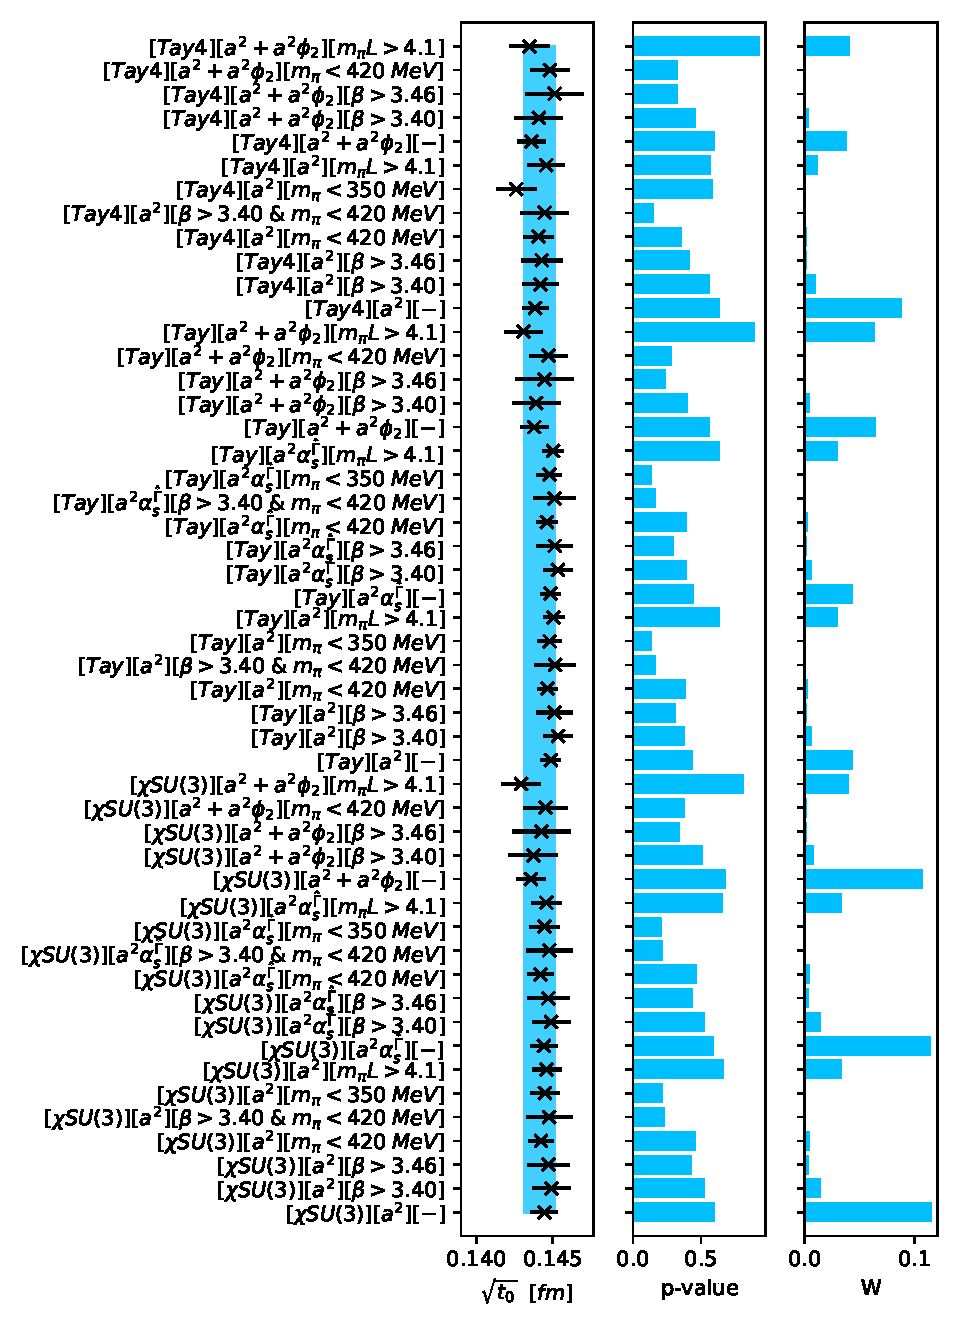
\includegraphics[width=1.\textwidth]{./cap5/figs/BMA_tm.pdf}
    \caption{Model average results for the determination of $\sqrt{t_0}$ at the physical point using the mixed action results. In the top figure we show the results coming from each fit model together with the final averaged result with the systematic uncertainty coming from the model variation added (blue band). In the middle plot we show the quality of fits as measured by the p-value~\cite{chi_exp}. In the bottom figure we show the assigned weight to each model according to eq.~(\ref{ch_ss:eq:W}). We provide a Table connecting each label to the corresponding fit models in Appendix~\ref{apex_model_av_t0}.}
    \label{ch_ss:fig:BMA_tm}
\end{figure}

\begin{figure}
    \centering
    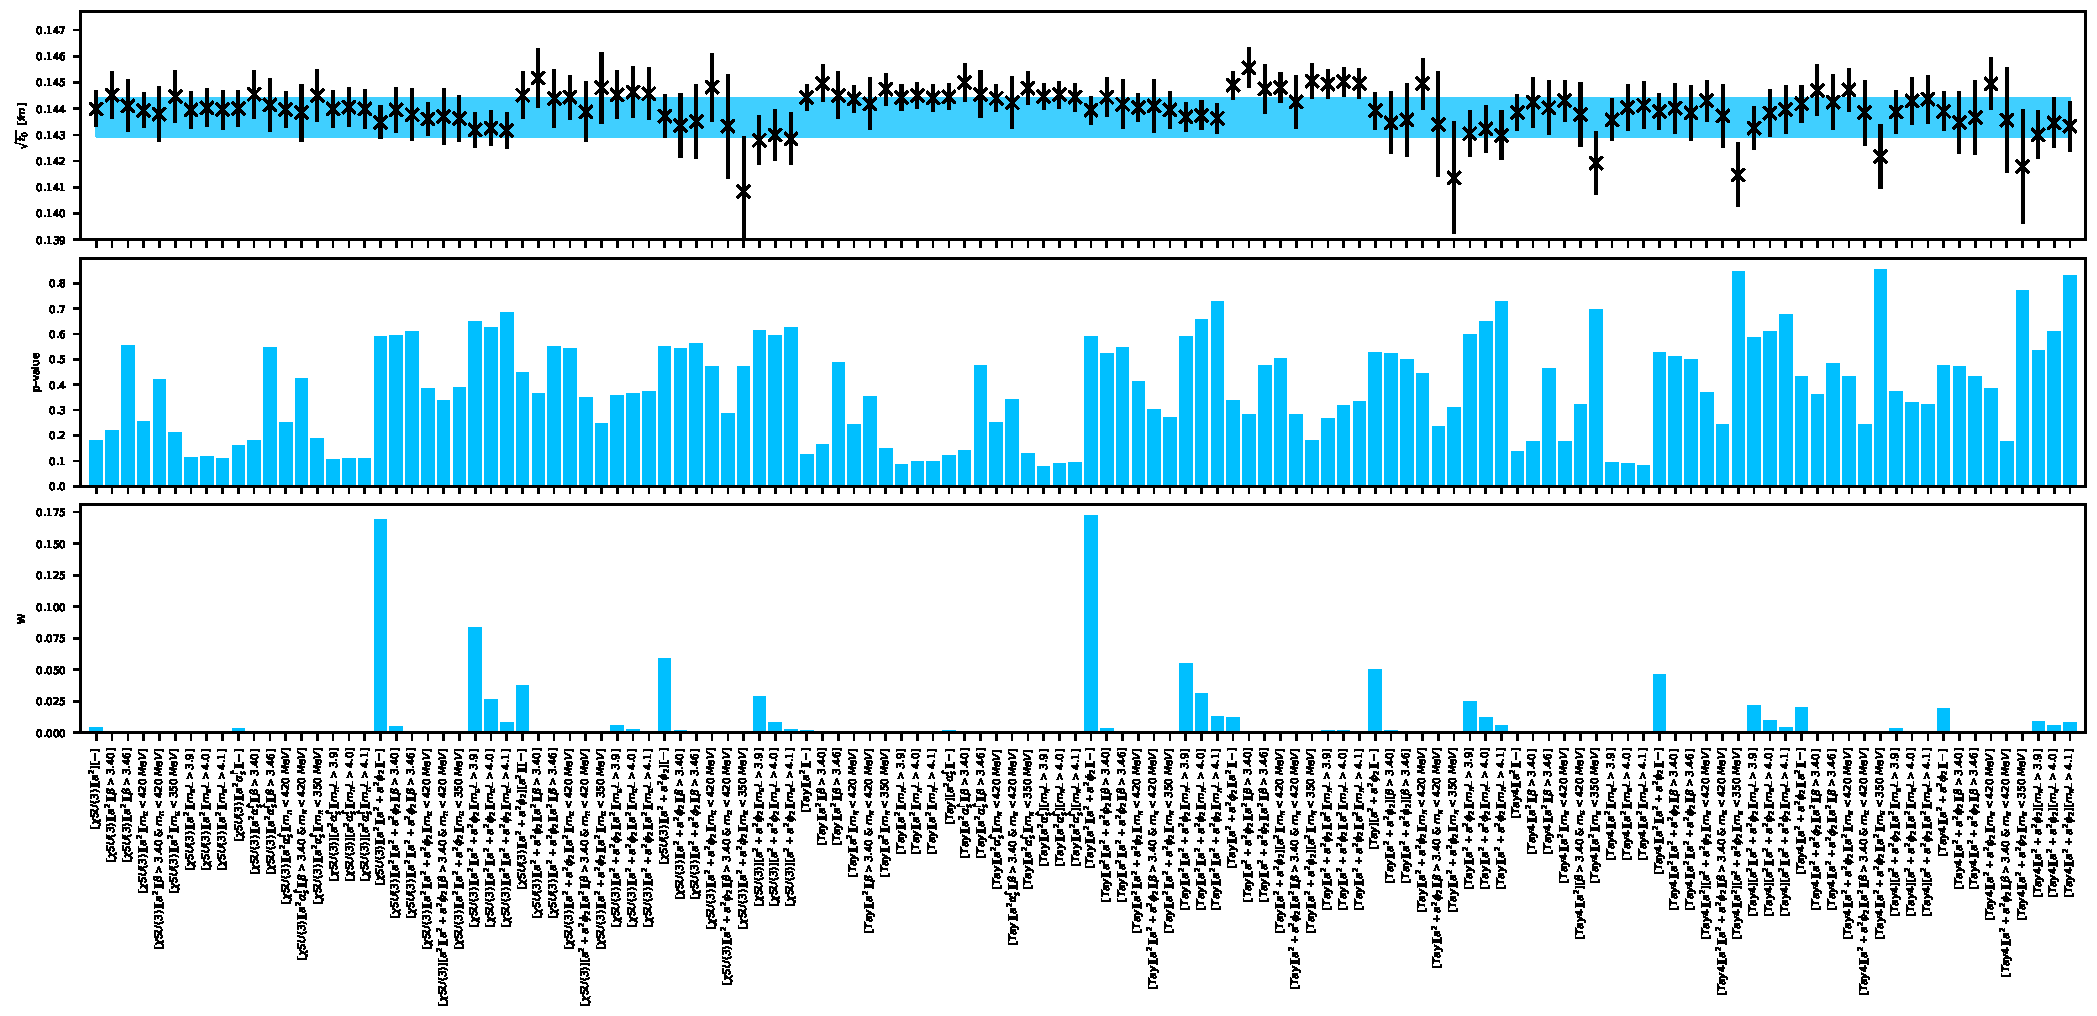
\includegraphics[width=1.\textwidth]{./cap5/figs/BMA_comb.pdf}
    \caption{Model average results for the determination of $\sqrt{t_0}$ at the physical point using the combined analysis of both Wilson and mixed action results. In the top figure we show the results coming from each fit model together with the final averaged result with the systematic uncertainty coming from the model variation added (blue band). In the middle plot we show the quality of fits as measured by the p-value~\cite{chi_exp}. In the bottom figure we show the assigned weight to each model according to eq.~(\ref{ch_ss:eq:W}). We provide a Table connecting each label to the corresponding fit models in Appendix~\ref{apex_model_av_t0}.}
    \label{ch_ss:fig:BMA_comb}
\end{figure}

\section{Results: the symmetric point}

The symmetric point is defined as the point in the quark mass plane such that
\begin{equation}
m_{ud}\equiv m_l=m_s.
\end{equation}
In terms of our usual quantities $\phi_2,\phi_4$ this means
\begin{equation}
\phi_2=\frac{2}{3}\phi_4,
\end{equation}
where $\phi_4$ again is given by its physical value after the iterative procedure to find $t_0^{\textrm{ph}}$ and after mass shifting (see Sec.~\ref{ch_ma:sec:chiral_traj}). In order to extract $t_0(\phi_2^{\textrm{sym}},\phi_4^{\textrm{ph}})$, following~\cite{•} we build the ratio
\begin{equation}
\frac{\sqrt{t_0/a^2}}{\sqrt{t_0^{\textrm{sym}}/a^2}},
\end{equation}
where $\sqrt{t_0/a^2}$ is the measurement of the gradient flow scale in each ensemble and $\sqrt{t_0^{\textrm{sym}}/a^2}$ is said quantity for the symmetric point at the corresponding value of the inverse coupling $\beta$. We now fit this ratio to
\begin{equation}
\label{ch_ss:eq:fit_t0_sym}
F(\phi_2)=\sqrt{1+p(\phi_2-\phi_2^{\textrm{sym}})}.
\end{equation}
Once the data is fitted, we extract $t_0^{\textrm{sym}}$ in physical units as
\begin{equation}
\sqrt{t_0^{\textrm{sym}}}=\frac{\sqrt{t_0^{\textrm{ph}}}}{F(\phi_2^{\textrm{ph}})}.
\end{equation}
For $t_0^{\textrm{ph}}$ and $\phi_2^{\textrm{ph}}$ we can use our determination for the Wilson, mixed action or combined data sets. The result of this fit is shown in Fig.~\ref{ch_ss:fig:t0_sym}. Our result for the scale at the symmetric point is
\begin{align}
\label{ch_ss:eq:t0_sym}
\sqrt{t_0^{\textrm{sym}}}&=0.1433(8)_{\textrm{stat}}(3)_{\textrm{syst}}\;\textrm{fm, Wilson}, \\
\sqrt{t_0^{\textrm{sym}}}&=0.1438(8)_{\textrm{stat}}(6)_{\textrm{syst}}\;\textrm{fm, Mixed action}, \\
\sqrt{t_0^{\textrm{sym}}}&=0.1437(6)_{\textrm{stat}}(4)_{\textrm{syst}}\;\textrm{fm, Combined}.
\end{align}

\begin{figure}
    \centering
    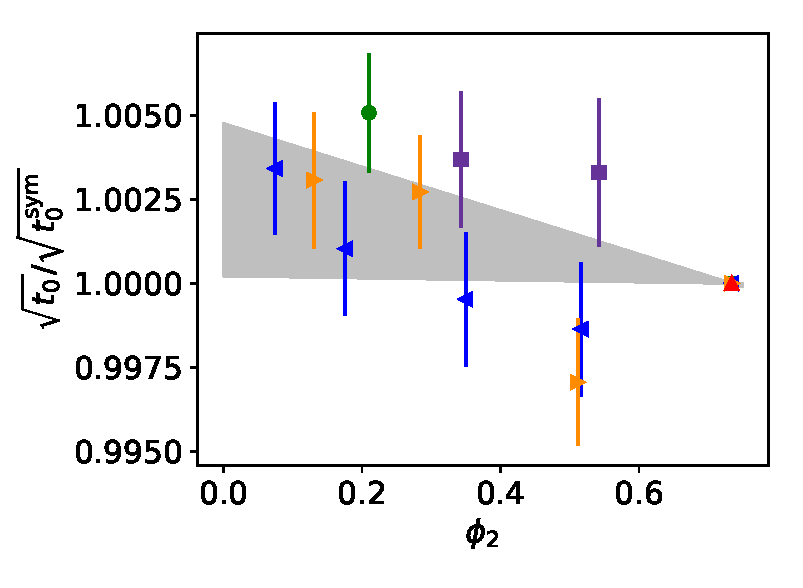
\includegraphics[width=.7\textwidth]{./cap5/figs/t0_sym.pdf}
    \caption{Fit to eq.~(\ref{ch_ss:eq:fit_t0_sym}) in order to extract $t_0$ at the symmetric point. The color and symbol code is the same as in Fig.~\ref{ch_ss:fig:SU3a2}.}
    \label{ch_ss:fig:t0_sym}
\end{figure}

\section{Results: lattice spacing}

Just as in the previous section, we can use the fit to $\frac{\sqrt{t_0/a^2}}{\sqrt{t_0^{\textrm{sym}}/a^2}}$ to compute 
\begin{equation}
\left(\sqrt{\frac{t_0}{a^2}}\right)^{\textrm{ph}}=\sqrt{\frac{t_0^{\textrm{sym}}}{a^2}}F(\phi_2^{\textrm{ph}}).
\end{equation}
Then, the lattice spacing is extracted as
\begin{equation}
\label{ch_ss:eq:a}
a=\frac{\sqrt{t_0^{\textrm{ph}}}}{\left(\sqrt{\frac{t_0}{a^2}}\right)^{\textrm{ph}}}.
\end{equation}
Again, for $\phi_2^{\textrm{ph}}$ we can use either our determination of $t_0^{\textrm{ph}}$ for the Wilson, mixed action or combined data sets. These results are shown in Table~\ref{ch_ss:tab:a}.

\begin{longtable}{c c c c}
\label{ch_ss:tab:a}
$\beta$ & $a$ [fm] Wilson & $a$ [fm] mixed action & $a$ [fm] combined \\
\toprule
$3.40$ & $0.0844(5)_{\textrm{stat}}(2)_{\textrm{syst}}$ & $0.0848(5)_{\textrm{stat}}(4)_{\textrm{syst}}$ & $0.0847(4)_{\textrm{stat}}(2)_{\textrm{syst}}$ \\
$3.46$ & $0.0749(4)_{\textrm{stat}}(2)_{\textrm{syst}}$ & $0.0752(4)_{\textrm{stat}}(3)_{\textrm{syst}}$ & $0.0751(3)_{\textrm{stat}}(2)_{\textrm{syst}}$ \\
$3.55$ & $0.0630(3)_{\textrm{stat}}(2)_{\textrm{syst}}$ & $0.0632(3)_{\textrm{stat}}(3)_{\textrm{syst}}$ & $0.0632(3)_{\textrm{stat}}(2)_{\textrm{syst}}$ \\
$3.70$ & $0.0489(3)_{\textrm{stat}}(1)_{\textrm{syst}}$ & $0.0490(3)_{\textrm{stat}}(2)_{\textrm{syst}}$ & $0.0490(2)_{\textrm{stat}}(1)_{\textrm{syst}}$ \\
$3.85$ & $0.0383(2)_{\textrm{stat}}(1)_{\textrm{syst}}$ & $0.0385(2)_{\textrm{stat}}(2)_{\textrm{syst}}$ & $0.0384(2)_{\textrm{stat}}(1)_{\textrm{syst}}$ \\
\bottomrule
\caption{Values of the lattice spacing $a$ in physical units extracted from the deterimation of the gradient flow scale $t_0$ with the Wilson, mixed action and combined analysis. The lattice spacing is extracted from measures of both $t_0$ at the physical and symmetric points using eq.~(\ref{ch_ss:eq:a}).}
\end{longtable}

\section{Results: $t_0^*$}

Following~\cite{•}, we define the gradient flow scale $t_0$ at the point
\begin{gather}
\phi_4=1.11, \quad \phi_2=\frac{2}{3}\phi_4\equiv\phi_2^{\textrm{sym}}.
\end{gather}
This defines $t_0^*$
\begin{equation}
t_0^*=t_0\left(\phi_2^{\textrm{sym}},\;\phi_4=1.11\right).
\end{equation}
This quantity is of importance for...~\cite{•} To compute it, we need to repeat the analysis above, this time mass shifting our ensembles to the value $\phi_4=1.11$ without errors and compute the gradient flow scale at the symmetric point as explained in the sections above.

The values we find for $\sqrt{t_0^*}$ in physical units for the Wilson, mixed action and combined cases are
\begin{align}
\label{ch_ss:eq:t0*}
\sqrt{t_0^*}&=0.1436(7)_{\textrm{stat}}(4)_{\textrm{syst}}\;\textrm{fm, Wilson}, \\
\sqrt{t_0^*}&=0.1441(7)_{\textrm{stat}}(5)_{\textrm{syst}}\;\textrm{fm, Mixed action}, \\
\sqrt{t_0^*}&=0.1438(6)_{\textrm{stat}}(3)_{\textrm{syst}}\;\textrm{fm, Combined}.
\end{align}

%%%%%%%%%%%%%%%%%%%%%%%%%%%%%%%%%%%%%%%%%%%%%%%%%%%%%%%%%%%
%%%%%%%%%%%%%%%%%%%%%%%%%%%%%%%%%%%%%%%%%%%%%%%%%%%%%%%%%%%
%%%%%%%%%%%%%%%%%%%%%%%%%%%%%%%%%%%%%%%%%%%%%%%%%%%%%%%%%%%
%%%%%%%%%%%%%%%%%%%%%%%%%%%%%%%%%%%%%%%%%%%%%%%%%%%%%%%%%%%

\chapter{Light quark masses}%\addcontentsline{toc}{chapter}{Light quark masses}

%%%%%%%%%%%%%%%%%%%%%%%%%%%%%%%%%%%%%%%%%%%%%%%%%%%%%%%%%%%
%%%%%%%%%%%%%%%%%%%%%%%%%%%%%%%%%%%%%%%%%%%%%%%%%%%%%%%%%%%
%%%%%%%%%%%%%%%%%%%%%%%%%%%%%%%%%%%%%%%%%%%%%%%%%%%%%%%%%%%
%%%%%%%%%%%%%%%%%%%%%%%%%%%%%%%%%%%%%%%%%%%%%%%%%%%%%%%%%%%

\label{ch_qm}

%%%%%%%%%%%%%%%%%%%%%%%%%%%%%%%%%%%%%%%%%%%%%%%%%%%%%%%%%%%
%%%%%%%%%%%%%%%%%%%%%%%%%%%%%%%%%%%%%%%%%%%%%%%%%%%%%%%%%%%
%%%%%%%%%%%%%%%%%%%%%%%%%%%%%%%%%%%%%%%%%%%%%%%%%%%%%%%%%%%
%%%%%%%%%%%%%%%%%%%%%%%%%%%%%%%%%%%%%%%%%%%%%%%%%%%%%%%%%%%

\section{Motivation}
\label{ch_qm:sec:introduction}

Blabla

%%%%%%%%%%%%%%%%%%%%%%%%%%%%%%%%%%%%%%%%%%%%%%%%%%%%%%%%%%%
%%%%%%%%%%%%%%%%%%%%%%%%%%%%%%%%%%%%%%%%%%%%%%%%%%%%%%%%%%%
%%%%%%%%%%%%%%%%%%%%%%%%%%%%%%%%%%%%%%%%%%%%%%%%%%%%%%%%%%%
%%%%%%%%%%%%%%%%%%%%%%%%%%%%%%%%%%%%%%%%%%%%%%%%%%%%%%%%%%%

\section{Results}
\label{ch_qm:sec:Results}

%%%%%%%%%%%%%%%%%%%%%%%%%%%%%%%%%%%%%%%%%%%%%%%%%%%%%%%%%%%
%%%%%%%%%%%%%%%%%%%%%%%%%%%%%%%%%%%%%%%%%%%%%%%%%%%%%%%%%%%

\cleardoublepage
\part{Conclusions}\label{pt:concl}
\chapter*{Conclusions and outlook}\addcontentsline{toc}{chapter}{Conclusions and outlook}
\markboth{CONCLUSIONS}{CONCLUSIONS}
\label{ch_conclu}

In this Ph.D. thesis we have obtained high precision results from first-principles Lattice QCD calculations of the gradient flow scale $t_0$ and the lattice spacing for CLS ensembles. This is relevant in modern day ``precision era'' Lattice Field Theory computations, since as the community is reaching sub-percent level precision in lattice predictions, setting the scale with the same accuracy is required, such that the scale is not the dominant source of uncertainty. In addition to this and following our scale setting procedure, we obtained high precision results for the renormalized charm quark mass and charmed mesons $D_{(s)}$ decay constants. In particular, these results are of utmost importance for high precision tests of the Standard Model and the search for New Physics, as they are expected to contribute to the detailed understanding of heavy quark dynamics in the Standard Model.

In this work we used CLS lattice gauge ensembles~\citep{Bruno:2014jqa,Mohler:2017wnb} with lattice spacings ranging from $a\approx0.085$ fm to $a\approx0.038$ fm, and pion masses from $m_{\pi}\approx420$ MeV to the physical point $m_{\pi}\approx130$ MeV. We have used a mixed action lattice regularization based on CLS gauge ensembles which uses $N_f=2+1$ $\mathcal{O}(a)$ improved Wilson quarks in the sea and $N_f=2+1+1$ Wilson twisted mass in the valence. We performed the matching of the mixed action through the pseudoscalar pion and kaon masses, which fixed equal physical quark masses for the up/down and strange quarks in the sea and valence sectors, treating the additional charm quark as a partially quenched flavor. This ensures unitarity of the theory in the continuum. Furthermore, we tuned the Wilson twisted mass parameters to impose maximal twist, ensuring automatic $\mathcal{O}(a)$ improvement~\citep{Frezzotti:2003ni,Shindler:2007vp} for valence observables up to negligible effects coming from the sea.

We employed the $\Gamma$-method to estimate errors from Monte Carlo data and automatic differentiation to perform exact error propagation. This allows to achieve control of autocorrelations and propagate errors into derived quantities. All these techniques are implemented by the ADerrors.jl Julia library~\citep{Ramos:2018vgu,Ramos:2020scv}. 

We have presented an update of the scale setting of this mixed action regularization and determined $t_0$ in physical units with finer lattice spacings and physical pion masses. For this task we employed the pion and kaon decay constants as physical input. We quote as final results for $t_0$
\begin{align}
\sqrt{t_0}&=0.1438(7)_{\textrm{stat}}(4)_{\textrm{syst}}\;\textrm{fm},\;[f_{\pi K}].
\end{align}
Using the kaon decay constant to set the scale relies on the determination of the CKM matrix element $V_{us}$ which has bigger uncertainty than $V_{ud}$. This large uncertainty affects the final result for the scale, in our case amounting to a $\sim11\%$ contribution to the total squared error. In addition to this, $f_K$ suffers from stronger QED corrections than $f_{\pi}$, whose uncertainty in our case amounts to a $\sim3\%$ contribution to the total squared error. For these reasons it is of utmost importance to determine the scale using only the decay constant of the pion, task for which physical point ensembles are of particular relevance. Currently our efforts are focused on this, as well as in the determination of the up/down and strange quark physical masses from a combination of the Wilson unitary and mixed action regularizations.

Furthermore, we have presented calculations of the determination of the physical charm quark mass and charmed mesons decay constants based on this mixed action setup, exploiting automatic $\mathcal{O}(a)$-improvement to reduce lattice artifacts associated with the heavy charm quark mass. Using our determination of the scale $t_0$ we quote as final results for the RGI charm quark mass in the three flavor theory
\begin{equation}
  M_c^{\mathrm{RGI}}(N_f=3) &=& 1.485(8)_{\textrm{stat}}(3)_{\textrm{syst}}(14)_{\textrm{RGI}}\ \mathrm{GeV}\,.
\end{equation}
Converting this result to the $\overline{\textrm{MS}}$ scheme in the four flavor theory for comparison with the literature we obtain
\begin{align}
  &M_c^{\mathrm{RGI}}(N_f=4) = 1.546(8)_{\textrm{stat}}(3)_{\textrm{syst}}(14)_{\textrm{RGI}}(4)_\Lambda(3)_{\rm trunc.} \ \mathrm{GeV}\,,\\
  &\overline{m}_c(\mu=3\ \mathrm{GeV}, N_f=4) = 1.006(5)_{\textrm{stat}}(2)_{\textrm{syst}}(9)_{\textrm{RGI}}(6)_\Lambda(3)_{\rm trunc.} \ \mathrm{GeV}\,,
	\\
	&\overline{m}_c(\mu=\overline{m}_c, N_f=4) = 1.296(5)_{\textrm{stat}}(2)_{\textrm{syst}}(8)_{\textrm{RGI}}(11)_\Lambda(5)_{\rm trunc.} \ \mathrm{GeV}\,.
\end{align}
The error of the RGI quark mass is completely dominated by the computation of the non-perturbative renormalization group running factor, and therefore, no substantial improvement can be achieved until a more precise calculation of this quantity is obtained.

For the $D_{(s)}$ decay constants we quote
\begin{align}
	f_D &= 211.3(1.9)_{\textrm{stat}}(0.6)_{\textrm{syst}} \ \mathrm{MeV},
	\\
	f_{D_s} &= 247.0(1.9)_{\textrm{stat}}(0.7)_{\textrm{syst}} \ \mathrm{MeV},
\end{align}
while for the ratio
\begin{equation}
	\frac{f_{D_s}}{f_D} = 1.177(15)_{\textrm{stat}}(5)_{\textrm{syst}}.
\end{equation}
In this case, the error is completely dominated by the statistical uncertainty of the gauge ensembles and the chiral-continuum extrapolations, and in the individual results for $f_{D_{(s)}}$ decay constants the scale setting accounts for the second largest contribution.

The results in the charm sector are based on a subset of the ensembles used for the scale setting. Currently we are focused on including the whole set of ensembles in Table~\ref{apex_ensembles:tab:ens} to the analysis of the charm sector.

We stress that the results obtained in this thesis are obtained in the isosymmetric QCD limit, defined in~\citep{FlavourLatticeAveragingGroupFLAG:2021npn}. Given the accuracy of our results, QED effects and strong isospin breaking effects are expected to be relevant, specially for charm observables. In future studies, where higher precision results can be achieved by increasing statistics and adding further ensembles, these effects will have to be taken into account.


\chapter*{Conclusiones y perspectivas}\addcontentsline{toc}{chapter}{Conclusiones y perspectivas}

En esta tesis doctoral hemos presentado un procedimiento de ajuste de escala o \textit{scale setting} en el contexto de QCD en el retículo que proporciona una nueva determinación de la escala $t_0$ y del espaciado reticular para configuraciones de campo gauge CLS. Una determinación precisa de la escala en el retículo es fundamental para alcanzar el nivel de precisión por debajo del $1\%$ requerido para algunos de los cálculos de QCD en el retículo destinados a mejorar la precisión de las predicciones del Modelo Estándar. Los resultados del \textit{scale setting} se están utilizando en un estudio en curso destinado a mejorar la determinación de las masas de los quarks y las constantes de desintegración de los mesones $D_{(s)}$. Estas cantidades son necesarias para mejorar la determinación de algunos de los parámetros fundamentales del Modelo Estándar y para reforzar las comprobaciones de consistencia de su validez.

En este trabajo hemos empleado configuraciones de campo gauge en el retículo generadas por la iniciativa CLS~\citep{Bruno:2014jqa,Mohler:2017wnb} con espaciados reticulares que van desde $a\approx0.085$ fm a $a\approx0.038$ fm, y masas de piones desde $m_{\pi}\approx420$ MeV hasta el punto físico $m_{\pi}\approx130$ MeV. Hemos utilizado una regularización reticular con una acción mixta basada en configuraciones gauge CLS con $N_f=2+1$ sabores de quarks Wilson $\mathcal{O}(a)$ \textit{improved} en el mar y $N_f=2+1+1$ sabores de quarks Wilson \textit{twisted mass} en la valencia. Realizamos el ajuste de la acción mixta a través de las masas pseudoescalares de piones y kaones, igualando las masas físicas para los quarks \textit{up/down} y \textit{strange} en los sectores mar y valencia, tratando el quark \textit{charm} adicional como un sabor parcialmente \textit{quenched}. Esto asegura la unitariedad de la teoría en el límite al continuo. Además, ajustamos los parámetros del operador de Dirac Wilson \textit{twisted mass} para imponer \textit{maximal twist}, asegurando así un $\mathcal{O}(a)$ \textit{improvement} automático~\citep{Frezzotti:2003ni,Shindler:2007vp} para observables de valencia, salvo efectos de orden superior procedentes del mar.

Empleamos el método--$\Gamma$ para calcular los errores de los datos Monte Carlo junto con herramientas de diferenciación automática para realizar una propagación de errores exacta a precisión de máquina. Esto permite considerar observables derivados arbitrariamente complejos, manteniendo un control adecuado de las autocorrelaciones. Estas técnicas se implementan dentro de la librería de Julia ADerrors.jl~\citep{Ramos:2018vgu,Ramos:2020scv}. 

Para el procedimiento de \textit{scale setting} basado en una combinación de las regularizaciones de Wilson y Wilson \textit{twisted mass} empleamos las constantes de desintegración del pión y el kaón como \textit{input} físico. Obtenemos el siguiente resultado para $\sqrt{t_0}$
\begin{equation}
\sqrt{t_0}=0.1441(6)_{\textrm{stat}}(4)_{\textrm{syst}}\;\textrm{fm},\;[f_{\pi K}].
\end{equation}
El uso de la constante de desintegración del kaón para establecer la escala $t_0$ depende de la determinación del elemento de la matriz CKM $|V_{us}|$, que tiene una incertidumbre mayor que $|V_{ud}|$. La incertidumbre de $|V_{us}|$ asciende a aproximadamente $6.5\%$ del error total al cuadrado de $\sqrt{t_0}$. Además, $f_K$ recibe mayores correcciones provenientes de QED que $f_{\pi}$, cuya incertidumbre asciende a una contribución de $\sim1.6\%$ al error total al cuadrado. Por lo tanto, es deseable considerar también el caso en el que solo la constante de desintegración del pión se utiliza como \textit{input} externo en el procedimiento de ajuste de escala. Se espera que el uso de configuraciones gauge simuladas a la masa física del pión con varios valores del espaciado reticular desempeñe un papel decisivo en dicho análisis. Esta sería una extensión natural del análisis presentado en este trabajo, junto con la determinación de las masas de los quarks \textit{up/down} y \textit{strange} a partir de una combinación de las regularizaciones unitaria y de acción mixta de Wilson, de las que proporcionamos un análisis preliminar en el Apéndice \ref{apex_light_qm}.


Además, siguiendo nuestro trabajo en ~\citep{charm} hemos presentado el estado actual de la determinación de la masa física del quark \textit{charm} y las constantes de decaimiento de los mesones $D_{(s)}$ basados en esta acción mixta, explotando el $\mathcal{O}(a)$ \textit{improvement} automático para reducir los artefactos reticulares asociados a la masa del quark pesado. Utilizando nuestra determinación de la escala $t_0$ citamos como resultado para la masa del quark \textit{charm} RGI en la teoría de tres sabores
\begin{equation}
  M_c^{\mathrm{RGI}}(N_f=3) &=& 1.486(8)_{\textrm{stat}}(3)_{\textrm{syst}}(14)_{\textrm{RGI}}\ \mathrm{GeV}\,.
\end{equation}
El error de la masa de quark RGI está dominado por el cálculo no-perturbativo del factor de \textit{running} del grupo de renormalización, y por lo tanto, no se puede conseguir una mejora sustancial hasta que se obtenga un cálculo más preciso de esta cantidad. En particular, la incertidumbre en la escala $t_0$ representa $\sim3\%$ del error total al cuadrado en $M_c^{\mathrm{RGI}}(N_f=3)$.

Para las constantes de desintegración $D_{(s)}$ citamos los siguientes resultados preliminares
\begin{align}
	f_D &= 211.1(1.8)_{\textrm{stat}}(0.5)_{\textrm{syst}} \ \mathrm{MeV},
	\\
	f_{D_s} &= 248.1(1.5)_{\textrm{stat}}(0.3)_{\textrm{syst}} \ \mathrm{MeV}.
\end{align}
En este caso, el error está dominado por la incertidumbre estadística de las configuraciones gauge y las extrapolaciones al punto físico y el límite al continuo, y la escala $t_0$ supone la segunda mayor contribución.

Los resultados obtenidos en este trabajo se obtuvieron en el límite de simetría de isospín de QCD, definido en~\citep{FlavourLatticeAveragingGroupFLAG:2021npn}. A medida que la precisión de los resultados de QCD en el retículo continúe mejorando, la inclusión de interacciones de QED y los efectos de ruptura del isospín fuerte son cada vez más relevantes para restringir los observables de la física de precisión. Otra vía para futuros desarrollos consiste en la extensión de la combinación de la regularización Wilson y de acción mixta para aproximarse al sector de quarks \textit{b}, siguiendo una estrategia de \textit{step-scaling} \cite{Sommer:2023gap}.




%\include{multiToC} % <--- just debug stuff, ignore for your documents
% ********************************************************************
% Backmatter
%*******************************************************
\appendix
%\renewcommand{\thechapter}{\alph{chapter}}
\cleardoublepage
\part{Appendix}
%%%%%%%%%%%%%%%%%%%%%%%%%%%%%%%%%%%%%%%%%%%%%%%%%%%%%%%%%%%
%%%%%%%%%%%%%%%%%%%%%%%%%%%%%%%%%%%%%%%%%%%%%%%%%%%%%%%%%%%
%%%%%%%%%%%%%%%%%%%%%%%%%%%%%%%%%%%%%%%%%%%%%%%%%%%%%%%%%%%
%%%%%%%%%%%%%%%%%%%%%%%%%%%%%%%%%%%%%%%%%%%%%%%%%%%%%%%%%%%

\chapter{Conventions}
\label{appex_conventions}

In this Appendix we set some useful notation used throughout this work. We begin with the Dirac or Gamma matrices $\gamma_{\mu}$, which are $4\times 4$ complex matrices defined by the anticommutator relation
\begin{equation}
\{\gamma_{\mu},\gamma_{\nu}\}=2g_{\mu\nu}1_{4\times 4},
\end{equation}
with $g_{\mu\nu}$ the metric tensor of 4-dimensional space-time. We will work in the Euclidean and flat space, so
\begin{equation}
g_{\mu\nu}=\textrm{diag}(+1,+1,+1,+1).
\end{equation}
Some useful properties of the Gamma matrices are
\begin{itemize}
\item Hermiticity: $\gamma_{\mu}^{\dagger}=\gamma_{\mu}$.
\item They are traceless: $\textrm{tr}(\gamma_{\mu})=0$.
\item Involutory: $\gamma_{\mu}^{-1}=\gamma_{\mu}$.
\end{itemize}
A fifth Gamma matrix can be defined as
\begin{equation}
\gamma_5=\gamma_0\gamma_1\gamma_2\gamma_3,
\end{equation}
which fulfills the same properties as above, and anticommutes with all other Gamma matrices
\begin{equation}
\{\gamma_5,\gamma_{\mu}\}=0.
\end{equation}

These matrices control the flavor content of hadrons, and as such appear in the definition of the lattice hadron interpolators. The relevant quark bilinears needed for this work are
\begin{itemize}
\item Scalar density: $S^{ij}=\bar{\psi}^i\psi^j$.
\item Pseudoscalar density: $P^{ij}=\bar{\psi}^i\gamma_5\psi^j$.
\item Axial current: $A_{\mu}^{ij}=\bar{\psi}^i\gamma_{\mu}\gamma_5\psi^j$.
\item Vector current: $V_{\mu}^{ij}=\bar{\psi}^i\gamma_{\mu}\psi^j$.
\end{itemize}
These bilinears are defined in the physical basis $\{\psi,\bar{\psi}\}$. By the change of variables
\begin{gather}
\psi\rightarrow e^{i\frac{\pi}{2}\gamma_5T/2}\psi, \quad \bar{\psi}\rightarrow\bar{\psi}e^{i\frac{\pi}{2}\gamma_5T/2},
\end{gather}
we define the twisted basis, with $T$ a diagonal matrix in flavor space. With this change of variables and at full twist with $N_f=2+1+1$
\begin{equation}
T=\textrm{diag}(+1,-1,-1,+1),
\end{equation}
the bilinears are rotated as 
\begin{align}
S^{ij}&\rightarrow S^{ij}, \\
P^{ij}&\rightarrow P^{ij}, \\
A_{\mu}^{ij}&\rightarrow iV_{\mu}^{ij}, \\
V_{\mu}^{ij}&\rightarrow -iA_{\mu}^{ij},
\end{align}
for $(i,j)=(u,d),(u,s),(c,d),(c,s)$, and
\begin{align}
S^{ij}&\rightarrow -iP^{ij}, \\
P^{ij}&\rightarrow iS^{ij}, \\
A_{\mu}^{ij}&\rightarrow A_{\mu}^{ij}, \\
V_{\mu}^{ij}&\rightarrow V_{\mu}^{ij},
\end{align}
for $(i,j)=(u,u),(u,c),(d,d),(d,s),(s,s),(c,c)$.

%%%%%%%%%%%%%%%%%%%%%%%%%%%%%%%%%%%%%%%%%%%%%%%%%%%%%%%%%%%
%%%%%%%%%%%%%%%%%%%%%%%%%%%%%%%%%%%%%%%%%%%%%%%%%%%%%%%%%%%
%%%%%%%%%%%%%%%%%%%%%%%%%%%%%%%%%%%%%%%%%%%%%%%%%%%%%%%%%%%
%%%%%%%%%%%%%%%%%%%%%%%%%%%%%%%%%%%%%%%%%%%%%%%%%%%%%%%%%%%


%%%%%%%%%%%%%%%%%%%%%%%%%%%%%%%%%%%%%%%%%%%%%%%%%%%%%%%%%%%
%%%%%%%%%%%%%%%%%%%%%%%%%%%%%%%%%%%%%%%%%%%%%%%%%%%%%%%%%%%
%%%%%%%%%%%%%%%%%%%%%%%%%%%%%%%%%%%%%%%%%%%%%%%%%%%%%%%%%%%
%%%%%%%%%%%%%%%%%%%%%%%%%%%%%%%%%%%%%%%%%%%%%%%%%%%%%%%%%%%


\chapter{Lattice ensembles}
\label{apex_ensembles}

\begin{longtable}{c c c c c c c c c c}
\label{apex_ensembles:tab:ens}
    id & $\beta$ & $m_{\pi}$ [MeV] & $m_K$ [MeV] & T/a & L/a & $m_{\pi}L$ & cnfg & BC & charm\\
    \toprule
    H101 & 3.40 & 421 & 421 & 96 & 32 & 5.8 & 1001,1009 & OBC & yes \\
    H102r001 & 3.40 & 355 & 442 & 96 & 32 & 4.9 & 997 & OBC & yes\\
    H102r002 & 3.40 & 360 & 445 & 96 & 32 & 5.0 & 1008 & OBC & yes\\
    H105 & 3.40 & 284 & 471 & 96 & 32 & 3.9 & 947,1042 & OBC & yes\\
    H105r005 & 3.40 & 286 & 467 & 96 & 32 & 3.9 & 837 & OBC & yes\\
\midrule
    H400 & 3.46 & 426 & 426 & 96 & 32 & 5.2 & 505,540 & OBC & yes\\
    D450 & 3.46 & 222 & 480 & 128 & 64 & 5.4 & 1000 & PBC & no\\
\midrule
    N202 & 3.55 & 416 & 416 & 128 & 48 & 6.4 & 899 & OBC & yes\\
    N203 & 3.55 & 348 & 446 & 128 & 48 & 5.4 & 756,787 & OBC & yes\\
    N200 & 3.55 & 287 & 468 & 128 & 48 & 4.4 & 856,856 & OBC & yes\\
    D200 & 3.55 & 203 & 486 & 128 & 64 & 4.2 & 2001 & OBC & yes\\
    E250 & 3.55 & 130 & 497 & 192 & 96 & 4.0 & 1009 & PBC & yes\\
\midrule
    N300r002 & 3.70 & 424 & 424 & 128 & 48 & 5.1 & 1521 & OBC & yes\\
    N302 & 3.70 & 348 & 453 & 128 & 48 & 4.2 & 2201 & OBC & yes\\
    J303 & 3.70 & 259 & 480 & 192 & 64 & 4.1 & 1073 & OBC & yes\\
    E300 & 3.70 & 176 & 496 & 192 & 96 & 4.2 & 1139 & OBC & yes\\ 
\midrule
    J500 & 3.85 & 417 & 417 & 192 & 64 & 5.2 & 789,655,431 & OBC & yes\\
    J501 & 3.85 & 340 & 453 & 192 & 64 & 4.3 & 1635,1142,1150 & OBC & yes\\
    \bottomrule
    \caption{List of CLS ensembles~\citep{Bruno:2014jqa,Mohler:2017wnb} under study. They use the Lüscher-Weisz gauge action defined in eq.~(\ref{ch_foundation:eq:LW}) and non-perturbatively $\mathcal{O}(a)$ improved $N_f=2+1$ Wilson fermions (see eq.~(\ref{ch_foundation:eq:DW_impr})). All ensembles use open boundary conditions (OBC) in time except for E250 and D450 (periodic), and periodic boundary conditions for all spatial directions. The last column refers to whether the corresponding ensemble is included or not in the analysis of charm physics in Chapter \ref{ch_charm}.}
\end{longtable}

%%%%%%%%%%%%%%%%%%%%%%%%%%%%%%%%%%%%%%%%%%%%%%%%%%%%%%%%%%%
%%%%%%%%%%%%%%%%%%%%%%%%%%%%%%%%%%%%%%%%%%%%%%%%%%%%%%%%%%%
%%%%%%%%%%%%%%%%%%%%%%%%%%%%%%%%%%%%%%%%%%%%%%%%%%%%%%%%%%%
%%%%%%%%%%%%%%%%%%%%%%%%%%%%%%%%%%%%%%%%%%%%%%%%%%%%%%%%%%%


%%%%%%%%%%%%%%%%%%%%%%%%%%%%%%%%%%%%%%%%%%%%%%%%%%%%%%%%%%%
%%%%%%%%%%%%%%%%%%%%%%%%%%%%%%%%%%%%%%%%%%%%%%%%%%%%%%%%%%%
%%%%%%%%%%%%%%%%%%%%%%%%%%%%%%%%%%%%%%%%%%%%%%%%%%%%%%%%%%%
%%%%%%%%%%%%%%%%%%%%%%%%%%%%%%%%%%%%%%%%%%%%%%%%%%%%%%%%%%%

\chapter{Simulation details}
\label{appex_simulations}

In this Appendix we discuss the details of the generation of gauge field configurations with dynamical quarks for the study of Lattice QCD. 

Typically simulations of lattice QCD with dynamical quarks require a large amount of computer resources due to the large number of degrees of freedom, the need for big volumes and small lattice spacings. The constant efforts by the community paved the way for simulations with up to four dynamical quarks. 

All ensembles studied in this thesis were generated using the openQCD software, and hence the details we review here are those of the algorithms implemented for this software~\citep{Luscher:2012av,Luscher:2010ae}.

As outlined in Sec.~\ref{ch_foundation:sec:path}, the expectation value of a composite operator $O$ can be computed in the lattice as
\begin{equation}
\left<O\right>=\frac{1}{\mathcal{Z}}\int\mathcal{D}[U]e^{-S_{\textrm{G}}[U]-S_{\textrm{eff}}[U]}O[U]\approx\frac{1}{N_{\textrm{cnfg}}}\sum_{i=1}^{N_{\textrm{cnfg}}}O[U_i]+\mathcal{O}\left(\frac{1}{\sqrt{N_{\textrm{cnfg}}}}\right),
\end{equation}
where the gauge fields $U_i$ are sampled from the probability density
\begin{equation}
\label{appex_simulations:eq:PU}
dP[U]=\frac{e^{-S_{\textrm{G}}[U]-S_{\textrm{eff}}[U]}}{\int\mathcal{D}[U]e^{-S_{\textrm{G}}[U]-S_{\textrm{eff}}[U]}}.
\end{equation}

The central idea is to perform an importance sampling of the distribution in eq.~(\ref{appex_simulations:eq:PU}), such that regions of field space with high probability are highly populated with gauge configurations $U_i$.  To achieve this, typically gauge configurations are generated following a Markov chain. This is defined as a sequence $\{U_k\}_{k=1}^{N_{\textrm{cnfg}}}$ such that the $k$-th element is generated from the previous one, with $k$ labeling the Monte Carlo (MC) time. This way, the Markov Chain is generated from the initial state $U_1$ and the transition probability $T(U_{k-1}\rightarrow U_k)$. Due to this gauge configurations in one same Markov Chain are highly correlated, issue which we deal with in Appendix~\ref{appex_errors}. The transition probabilities must obey the following conditions:
\begin{itemize}
\item Ergodicity: given a subset of states $S$ from the Markov Chain, there are always at least two states $s\in S$ and $s'\notin S$ with $T(s\rightarrow s')>0$. This is of particular importance in the context of Lattice QCD and Lattice Yang-Mills theories in order to ensure that the simulation algorithm is sampling correctly all topological sectors of the theory, which may not always be the case for different algorithms.
\item Equilibrium: normalizing the transition probability as
\begin{equation}
\sum_sT(s\rightarrow s')=1\;\;\;\;\forall s,
\end{equation}
then it must hold that
\begin{equation}
\sum_sP(s)T(s\rightarrow s')=P(s')\;\;\;\;\forall s',
\end{equation}
where $P(s)$ is the equilibrium distribution in eq.~(\ref{appex_simulations:eq:PU}). This ensures that starting from a random configuration, after applying iteratively the transition probability, we asymptotically reach the target equilibrium distribution in eq.~(\ref{appex_simulations:eq:PU}). 
\end{itemize}

Different choices for the transition probability $T(s\rightarrow s')$ satisfying the above conditions define the different sampling algorithms which we go on to review. 

\section{Metropolis algorithm}

The Metropolis algorithm~\citep{Metropolis:1953am} is one of the most popular choices for generating a Markov Chain of gauge field configurations for pure gauge theories, for which the target distribution is
\begin{equation}
dP[U]=\frac{e^{-S_{\textrm{G}}[U]}}{\int\mathcal{D}[U]e^{-S_{\textrm{G}}[U]}}.
\end{equation}
The idea is to define an a priori selection probability $T_0(U_i\rightarrow U_j)$ to update a single gauge link. One such choice is to take a random element $g$ of the $SU(N)$ group close to the identity and update the gauge link $U_{\mu}(n)$ as $U_{\mu}(n)'=gU_{\mu}(n)$ such that the new gauge configuration $U_j$ is close to the original one $U_i$. In order for the transition to be symmetric, group elements $g$ and $g^{-1}$ have to be selected with equal probability. After updating with this a priori transition probability, one supplements the updating process with an accept-reject step, such that the new proposed gauge link is accepted with probability
\begin{gather}
P_{\textrm{acc}}(i,j)=\textrm{min}\left(1,e^{-\Delta S}\right), \quad \Delta S=S[U_j]-S[U_i].
\end{gather}
Then the total transition probability is given by 
\begin{equation}
T(U_i\rightarrow U_j)=T_0(U_i\rightarrow U_j)P_{\textrm{acc}}(i,j)+\delta_{ij}\sum_kT_0(U_i\rightarrow U_j)(1-P_{\textrm{acc}}(i,j)).
\end{equation}
This $T$ satisfies all the desired properties for a transition probability and asymptotically reaches the target distribution probability for pure gauge theories.

The drawback of this algorithm is that it only updates a single gauge link at each step and as such is highly inefficient, particularly for large volume simulations. Over the years new alternatives for pure gauge simulations have been proposed, such as the heat bath~\citep{Creutz:1980zw} and overrelaxation~\citep{Adler:1981sn,Creutz:1987xi} algorithms.

\section{Hybrid Monte Carlo}

Having as target distribution that of pure gauge theory is equivalent as treating quarks in the sea as static sources (infinitely heavy). In order to simulate full QCD, one needs to have dynamical quarks in the sea, meaning having target distribution eq.~(\ref{appex_simulations:eq:PU}), where $S_{\textrm{eff}}$ introduces non-local dependencies in the gauge links due to the quark determinant. Therefore algorithms like Metropolis, which updates the gauge configurations link by link, experience a significant computational cost that increases with the lattice volume squared, which makes the algorithm unpractical for dynamical simulations purposes. The Hybrid Monte Carlo (HMC) algorithm~\citep{Duane:1987de,Gottlieb:1987mq} significantly improves efficiency by doing global updates of the gauge configurations.

The HMC uses the classical equations of motion to propose new gauge configurations. To this purpose, the field space is extended with the introduction of the conjugate momenta $\pi_{\mu}(x)$ of the link variables $U_{\mu}(x)$. The Hamiltonian of the system is
\begin{equation}
H[\pi,U]=\frac{1}{2}\sum_{x,\mu}\pi_{\mu}^a(x)\pi_{\mu}^a(x)+S_{\textrm{G}}[U]+S_{\textrm{eff}}[U].
\end{equation}
This way expectation values can be computed as
\begin{equation}
\left<O\right>=\frac{\int\mathcal{D}[\pi,U]e^{-H[\pi,U]}O[U]}{\int\mathcal{D}[\pi,U]e^{-H[\pi,U]}}.
\end{equation}
Now the classical equations of motion read
\begin{gather}
\dot{\pi}_{\mu}(x)=-F_{\mu}(x), \quad F_{\mu}(x)=\left.\frac{\partial S[e^{\omega}U]}{\partial\omega}\right|_{\omega=0}, \quad \omega\in su(N), \\
\dot{U}_{\mu}(x)=\pi_{\mu}(x)U_{\mu}(x),
\end{gather}
where the dot notation ``$\dot{a}$'' means derivation with respect to MC time. This way, starting from an initial configuration at zero MC time, integrating the equations of motion provides with a global new gauge configuration to be used as proposal for the update of the gauge links. This new global proposal is subject to an accept-reject step like the one in the Metropolis algorithm with
\begin{gather}
P_{\textrm{acc}}=\textrm{min}\left(1,e^{-\Delta H}\right), \quad \Delta H=H[\pi',U']-H[\pi,U].
\end{gather}

We have presented the basic formulation of the HMC algorithm but further refinements and improvements, specially in terms of the integration of the classical equations of motion have taken place over the years~\citep{Weingarten:1991ra,OMELYAN2003272,Hasenbusch:2001ne}.

This far we have not given details on how to compute the effective fermion action
\begin{equation}
S_{\textrm{eff}}[U]=-\sum_{i=1}^{N_f}\textrm{log det}(D_i).
\end{equation}
This is a typically challenging task, since it involves dealing with Grassmann variables. A popular solution is to use pseudofermion fields $\Phi(x)$~\citep{Weingarten:1980hx}, which are auxiliary fields that carry color and spinor indices $c,\alpha$ but that are complex instead of Grassmann numbers. Restricting to the mass-degenerate doublet of light quarks, where the effective action becomes
\begin{equation}
e^{-S_{\textrm{eff}}}=\textrm{det}(D_l)\textrm{det}(D_l)=\textrm{det}(D_l^{\dagger}D_l),
\end{equation}
in the pseudo-fermion representation this becomes
\begin{equation}
\textrm{det}(D_l^{\dagger}D_l)=\frac{1}{\mathcal{Z}_{\Phi}}\int\mathcal{D}[\Phi]e^{-S_{\textrm{pf}}[U,\Phi]},
\end{equation}
with $\mathcal{Z}_{\Phi}$ the pseudo-fermion partition function, and the pseudo-fermion action given by
\begin{equation}
S_{\textrm{pf}}[U,\Phi]=\Phi^{\dagger}\left(D_l^{\dagger}D_l\right)^{-1}\Phi.
\end{equation}

Now we have all ingredients needed for HMC sampling with dynamical fermions. First one samples randomly a set of conjugate momenta $\pi_{\mu}$ and pseudo-fermion fields $\Phi$ with Gaussian distribution $\propto\exp\left(-\frac{1}{2}\pi_{\mu}\pi_{\mu}-S_{\textrm{pf}}\right)$. Together with an initial gauge field configuration $U_{i}$, the classical equations of motion are integrated up to some later time. At this point one implements the accept-reject step and updates the gauge configuration to $U_{i+1}$.

This far we assumed two degenerate flavors of quarks to compute the effective fermion action. The inclusion of a strange quark, as in the case of the CLS ensembles we use in this work, complicates things since it does not belong to a mass-degenerate doublet, and thus one needs to compute $\textrm{det}(D_s)$ and not $\textrm{det}(D_l^{\dagger}D_l)$. When this happens the quark determinant is not ensured to be positive anymore due to explicit chiral symmetry breaking by the Wilson term in Wilson quarks. This is of particular relevance because if the strange quark determinant gets a negative value one cannot interpret the factor $e^{-S_{\textrm{G}}-S_{\textrm{eff}}}$ appearing in the path integral as a probability. In CLS ensembles this difficulty is tackled by the Rational Hybrid Monte Carlo algorithm~\citep{Kennedy:1998cu,Clark:2006fx}. However, in~\citep{Mohler:2020txx} it was found that some configurations still suffered from a negative strange quark determinant. In this case we introduce a reweighting factor with minus sign to account for the effect. Reweighting is discussed in the next section.

\section{Reweighting}

The idea of reweighting was first proposed in~\citep{Luscher:2008tw} in order to deal with exceptional gauge configurations in the HMC algorithm. These are gauge configurations with near to zero eigenvalues for the Dirac operator, which can appear due to the explicit chiral symmetry breaking induced by the Wilson term in the Wilson fermion action.

In the context of CLS ensembles, a small twisted mass term $\mu_0$ is included in the light quark determinant as~\citep{Luscher:2012av}
\begin{equation}
\textrm{det}\left(Q^{\dagger}Q\right)\rightarrow\textrm{det}\left(\left(Q^{\dagger}Q+\mu_0^2\right)^2\left(Q^{\dagger}Q+2\mu_0^2\right)^{-1}\right),
\end{equation}
with the Hermitian Dirac operator given by $Q=\gamma_5D$. This provides an infrared cutoff to cancel low-mode eigenvalues. Using the Hasenbusch’s mass factorization~\citep{Hasenbusch:2001ne}
\begin{align}
&\textrm{det}\left(\left(Q^{\dagger}Q+\mu_0^2\right)^2\left(Q^{\dagger}Q+2\mu_0^2\right)^{-1}\right) \\ 
&=\textrm{det}\left(Q^{\dagger}Q+\mu_{n}^2\right)\textrm{det}\left(\frac{Q^{\dagger}Q+\mu_{0}^2}{Q^{\dagger}Q+2\mu_0^2}\right)\times\Pi_{i=1}^{n}\textrm{det}\left(\frac{Q^{\dagger}Q+\mu_{i-1}^2}{Q^{\dagger}Q+\mu_i^2}\right),
\end{align}
where the twisted mass factors are ordered as $\mu_0<\mu_1<...<\mu_{n}$. We used $\gamma_5$-hermiticity of the Dirac operator $D$ so that
\begin{equation}
Q^{\dagger}Q=\gamma_5D^{\dagger}\gamma_5D=D^{\dagger}D.
\end{equation}
The values of the twisted mass factors have to be properly chosen as large values might lead to large fluctuations and poor efficiency of the algorithm. After introducing such twisted masses, in order to account for their effect and recover the target desired distribution $dP[U]$ of QCD (in which this twisted mass is not present) a reweighting of expectation values over gauge configurations is needed
\begin{equation}
\left<O\right>_{\textrm{rw}}=\frac{\left<OW\right>}{\left<W\right>},
\end{equation}
where $W$ is the reweighting factor and in this case reads
\begin{equation}
W=\textrm{det}\left(Q^{\dagger}Q\left(Q^{\dagger}Q+2\mu_0^2\right)\left(Q^{\dagger}Q+\mu_0^2\right)^{-2}\right).
\end{equation}

In addition to twisted mass reweighting, reweighting is also needed due to the use of the RHMC algorithm to simulate the strange quark determinant. This algorithm uses the rational approximation to the strange quark determinant~\citep{RHMC}, which is expected to make it positive. However, as mentioned in the previous section, in~\citep{Mohler:2020txx} it was found that some configurations still got a negative sign for the strange quark determinant. This is solved by a reweighting factor of $W_s=-1$ for said configurations, which we list in Table~\ref{tab:Ws} for the ensembles of interest in this thesis.

\begin{longtable}{c | c}
\toprule
id & cnfg \\
\
H105r001 & 3 \\
H105r002 & 1 \\
H105r005 & 254, 255, 256, 257, 259, 260, 261, 264, \\
         & 265, 266, 269, 280, 282, 283, 284, 285, \\
         & 286, 287, 288, 289, 291, 299, 301, 313,\\
         & 314, 315, 316, 331, 332, 333, 334, 335, \\
         & 336, 337, 338, 339, 340, 341, 342  \\
J303r003 & 324, 325, 326 \\
\bottomrule
\caption{List of configurations with negative sign of the strange quark determinant for each affected ensemble in this study. A reweighting factor $W_s=-1$ is introduced in said configuration in order to account for the effect~\citep{Mohler:2020txx}.}
\label{tab:Ws}
\end{longtable}

%%%%%%%%%%%%%%%%%%%%%%%%%%%%%%%%%%%%%%%%%%%%%%%%%%%%%%%%%%%
%%%%%%%%%%%%%%%%%%%%%%%%%%%%%%%%%%%%%%%%%%%%%%%%%%%%%%%%%%%
%%%%%%%%%%%%%%%%%%%%%%%%%%%%%%%%%%%%%%%%%%%%%%%%%%%%%%%%%%%
%%%%%%%%%%%%%%%%%%%%%%%%%%%%%%%%%%%%%%%%%%%%%%%%%%%%%%%%%%%


%%%%%%%%%%%%%%%%%%%%%%%%%%%%%%%%%%%%%%%%%%%%%%%%%%%%%%%%%%%
%%%%%%%%%%%%%%%%%%%%%%%%%%%%%%%%%%%%%%%%%%%%%%%%%%%%%%%%%%%
%%%%%%%%%%%%%%%%%%%%%%%%%%%%%%%%%%%%%%%%%%%%%%%%%%%%%%%%%%%
%%%%%%%%%%%%%%%%%%%%%%%%%%%%%%%%%%%%%%%%%%%%%%%%%%%%%%%%%%%

\chapter{Error analysis}
\label{apex_errors}

In this appendix we discuss how to perform the data analysis of correlation functions and the different lattice observables extracted from lattice simulations. 

Lattice data is measured from Monte Carlo (MC) sampling, and estimates of expectation values of physical observables are extracted from means over the MC time. A crucial step is to assign a proper statistical and systematic uncertainties to these mean values, for which it is needed to take into account the autocorrelated nature of MC measurements. This autocorrelation arises form the fact that each gauge configuration is proposed from the previous one (Markov chain). Some popular methods to deal with these correlations are binning, bootstrap and the jack-knife methods~\cite{}.

A recent technique which we will use in this work was proposed by the ALPHA collaboration~\cite{Gamma-method} and is known as $\Gamma$-method, which explicitely computes the autocorrelation function to estimate the statistical uncertainty.

In lattice simulations tipically one measures a primary observable $p_i$ over several ensembles (defined by the simulation parameters like e.g. the inverse coupling $\beta$ and $\kappa$ parameter) 
\begin{equation}
p_i^{\alpha}(k), k=1,...,N_{\alpha},
\end{equation}
where $\alpha$ labels the ensemble and $k$ is the MC time running over the total number of gauge configurations $N_{\alpha}$ of the given ensemble. In our context, primary observable means a correlation function for some given euclidean time. An estimate for the true value $P_i^{\alpha}$ is given by the mean value
\begin{equation}
\bar{p}_i^{\alpha}=\frac{1}{N_{\alpha}}\sum_{k=1}^{N_{\alpha}}p_i^{\alpha}(k)\rightarrow_{N_{\alpha}\rightarrow\infty}P_i^{\alpha}.
\end{equation}
This is an unbiased estimator. Fluctuations over the MC time can be computed as
\begin{equation}
\delta_i^{\alpha}(k)=p_i^{\alpha}(k)-\bar{p}_i^{\alpha}.
\end{equation}
Due to the Central Limit theorem, we are ensured that $\bar{p}_i^{\alpha}$ behaves as a Gaussian distribution independently of the distribution of $p_i^{\alpha}(k)$, and so the statistical uncertainty associated to $\bar{p}_i^{\alpha}$ is simply given by the standard deviation $\sigma_i^{\alpha}$,
\begin{equation}
P_i^{\alpha}\approx\bar{p}_i^{\alpha}\pm\sigma_i^{\alpha}.
\end{equation}
This standard deviation can be computed from the autocorrelation $\Gamma$ function
\begin{equation}
(\sigma_i^{\alpha})^2=\frac{1}{N_{\alpha}}\sum_{k=-\infty}^{\infty}\Gamma_{ii}^{\alpha\alpha}(k),
\end{equation}
where the $\Gamma$ function is defined as
\begin{equation}
\Gamma_{ij}^{\alpha\beta}=\frac{\delta_{\alpha\beta}}{N_{\alpha}-k}\sum_{k'=1}^{N_{\alpha}-k}\delta_i^{\alpha}(k+k')\delta_j^{\alpha}(k').
\end{equation}

From the primary observable $p_i^{\alpha}$ we can compute derived observables $F=f(p_i^{\alpha})$, such as meson masses coming from pseudoscalar two point functions. As in the primary observable case, we can estimate this derived observable as
\begin{equation}
\bar{F}=f(\bar{p}_i^{\alpha}).
\end{equation}
To compute the statistical uncertainty, we can expand $f$ around the true value $P_i^{\alpha}$
\begin{equation}
f(P_{i}^{\alpha}+\epsilon_{i}^{\alpha})=f(P_{i}^{\alpha})+\bar{f}_i^{\alpha}\epsilon_{i}^{\alpha}+\mathcal{O}((\epsilon_{i}^{\alpha})^2),
\end{equation}
with
\begin{equation}
\bar{f}_i^{\alpha}=\frac{\partial f(x)}{\partial x}|_{x=P_{i}^{\alpha}}.
\end{equation}
Now the autocorrelation function of the derived observable $F$ for ensemble $\alpha$ can be defined as
\begin{equation}
\Gamma_F^{\alpha}(k)=\sum_{ij}\bar{f}_i^{\alpha}\bar{f}_j^{\alpha}\Gamma_{ij}^{\alpha\alpha}(k),
\end{equation}
from which the standard deviation of $F$ can be derived
\begin{equation}
\sigma_F^2=\sum_{\alpha}\frac{\Gamma_F^{\alpha}(0)}{N_{\alpha}}2\tau_{\textrm{int}}^{\alpha}(F),
\end{equation}
where we assumed that several ensembles contribute to $F$, and hence the sum $\sum_{\alpha}$ over the subset of them which contribute. The integrated autocorrelation time $\tau_{\textrm{int}}^{\alpha}(F)$ is defined as
\begin{equation}
\label{app_errors:eq:taui}
\tau_{\textrm{int}}^{\alpha}(F)=\frac{1}{2}+\sum_{k=1}^{\infty}\frac{\Gamma_F^{\alpha}(k)}{\Gamma_F^{\alpha}(k)}.
\end{equation}
To estimate it, a truncation in MC time $k$ is needed. The autocorrelation function admits the following expansion~\cite{•}
\begin{equation}
\Gamma(k)\approx\sum_{n=0}^{\infty}e^{-k/\tau_n}.
\end{equation}
The slowest mode $\tau_0\equiv\tau_{\textrm{exp}}$ is called the exponential autocorrelation time and it gives the decay rate of $\Gamma(k)$. Truncating eq.~(\ref{app_errors:eq:taui}) at MC time $k=W_F^{\alpha}$ introduces a systematic uncertainty of $\mathcal{O}(\exp(-W_F^{\alpha}/\tau_{\textrm{exp}}^{\alpha}))$. The $\Gamma$-method proposes as optimal window that which minimizes the sum of statistical and systematic contributions
\begin{equation}
W_F^{\alpha}=min_W\left(e^{-W/\tau_{\textrm{exp}}^{\alpha}}+...?\right).
\end{equation}
In~\cite{•} it was proposed to set $\tau_{\textrm{exp}}=S_{\tau}\tau_{\textrm{int}}$, with $S_{\tau}$ some value between 2 and 5. One can also vary $W_F^{\alpha}$ until saturation in $\tau_{\textrm{int}}^{\alpha}$ is reached. In~\cite{•} it was also proposed to add an exponential tail
\begin{equation}
\tau_{\textrm{exp}}^{\alpha}\frac{\Gamma_F^{\alpha}(W_F^{\alpha}+1)}{\Gamma_F^{\alpha}(0)},
\end{equation}
to eq.~\ref{app_errors:eq:taui} to account for the systematic effect of truncating the sum over MC time. For this an estimate of $\tau_{\textrm{exp}}^{\alpha}$ is needed for each ensemble. In the case of CLS ensembles an estimation is given in~\cite{}
\begin{equation}
\tau_{\textrm{exp}}^{\alpha}=14(3)\frac{t_0}{a^2}.
\end{equation}

In this thesis we use the $\Gamma$-method explained above as it is implemented by the ADerrors.jl julia package~\cite{•}.


%%%%%%%%%%%%%%%%%%%%%%%%%%%%%%%%%%%%%%%%%%%%%%%%%%%%%%%%%%%
%%%%%%%%%%%%%%%%%%%%%%%%%%%%%%%%%%%%%%%%%%%%%%%%%%%%%%%%%%%
%%%%%%%%%%%%%%%%%%%%%%%%%%%%%%%%%%%%%%%%%%%%%%%%%%%%%%%%%%%
%%%%%%%%%%%%%%%%%%%%%%%%%%%%%%%%%%%%%%%%%%%%%%%%%%%%%%%%%%%


%%%%%%%%%%%%%%%%%%%%%%%%%%%%%%%%%%%%%%%%%%%%%%%%%%%%%%%%%%%
%%%%%%%%%%%%%%%%%%%%%%%%%%%%%%%%%%%%%%%%%%%%%%%%%%%%%%%%%%%
%%%%%%%%%%%%%%%%%%%%%%%%%%%%%%%%%%%%%%%%%%%%%%%%%%%%%%%%%%%
%%%%%%%%%%%%%%%%%%%%%%%%%%%%%%%%%%%%%%%%%%%%%%%%%%%%%%%%%%%

\chapter{Solvers}
\label{appex_solvers}

For the computation of correlation functions of fermions in the lattice (e.g. a two-point function, see eq.~(\ref{ch_foundation:eq:path_int})) the inversion of the Dirac operator is required. In particular it is needed to compute the inverse of $D(x,y)$ for all spatial positions $\vec{x},\vec{y}$. This is referred to as inverting the all-to-all Dirac operator. This is computationally very expensive, and stochastic methods can be employed to reduce the computational cost. A set of stochastic noise sources $\eta$ are introduced such that
\begin{gather}
\left<\eta_i(x)\right>_{\eta}=0, \quad \left<\eta_i^{\dagger}(x)\eta_j(y)\right>_{\eta}=\delta_{x,y}\delta_{i,j},
\end{gather}
with $\left<.\right>_{\eta}$ meaning average over the $N_{\eta}$ samples of some noise distribution. Some common choices are gaussian, $Z_2$ or $U(1)$. From these we define
\begin{gather}
\xi_i^q(x)=\sum_yD^{-1}_q(x,y)\eta_i(y), \quad \zeta_i^r(x)=\sum_yD^{-1}_r(x,y)\gamma_5\Gamma_B^{\dagger}\eta_i(y),
\end{gather}
with $\Gamma_B$ some Gamma matrix. Now, two-point functions like the one in eq.~(\ref{ch_foundation:eq:path_int})) can be expressed as
\begin{align}
\left<O^{rq}_AO^{qr}_B\right>&-\frac{a^6}{L^3}\sum_{\vec{y}}\left<\left<(\Gamma_A\gamma_5\zeta^r_i(y))^{\dagger}\xi^q_i(y)\right>_{\eta}\right> \\
&\approx -\frac{a^6}{L^3}\frac{1}{N_{\eta}}\sum_{i=1}^{N_{\eta}}\sum_{\vec{y}}\left<(\Gamma_A\gamma_5\zeta^r_i(y))^{\dagger}\xi^q_i(y)\right>,
\end{align}
without the need to compute the all-to-all inverted Dirac operator, therefore reducing significantly the computational effort.

In order to invert the Dirac operator with flavor $q$, the solution to the Dirac equation 
\begin{equation}
D_q(x,y)\psi_r(y)=\delta_{x,y}\delta_{q,r}\equiv\eta_{x,y,q,r},
\end{equation}
must be found. This is usually done by an iterative procedure. The basic idea is to start from an initial approximate solution $\psi_0$ and define the residue $\rho$ (we supress indices for simplicity)
\begin{equation}
\rho=D\psi_0-\eta.
\end{equation}
Then, one solves
\begin{equation}
D\psi_1=\rho,
\end{equation}
finding the new residue and iterates the process, with the final approximate solution given by
\begin{equation}
\psi=\psi_0+\psi_1+...
\end{equation}
The algorithm stops when some convergence criterion is met
\begin{equation}
|\rho|<\epsilon.
\end{equation}
The difference between the true and approximate solutions is
\begin{equation}
|\psi-\psi_{\textrm{true}}|<\epsilon\kappa(D),
\end{equation}
with $\kappa(D)$ the condition number of matrix $D$
\begin{equation}
\kappa(D)=|D||D^{-1}|.
\end{equation}
The smaller the condition number of the Dirac operator, the less iterative steps one needs to perform in order to find the solution to the Dirac equation. Thus convergence can be improved by suitably transforming the system into one with a smaller $\kappa(D)$. This can be done by finding some similarity transformations easily invertible such that one can write
\begin{gather}
LDR\psi'=L\eta, \quad \psi=R^{-1}\psi'.
\end{gather}
This is called preconditioning, and there are many different variations. Some of the most used are even-odd preconditioning~\cite{•} and distance preconditioning~\cite{•}.

There are also more sophisticated algorithms to solve the Dirac equation based on conjugate gradient solvers~\cite{•} and the Krylov subspace solvers~\cite{•}.

%%%%%%%%%%%%%%%%%%%%%%%%%%%%%%%%%%%%%%%%%%%%%%%%%%%%%%%%%%%
%%%%%%%%%%%%%%%%%%%%%%%%%%%%%%%%%%%%%%%%%%%%%%%%%%%%%%%%%%%
%%%%%%%%%%%%%%%%%%%%%%%%%%%%%%%%%%%%%%%%%%%%%%%%%%%%%%%%%%%
%%%%%%%%%%%%%%%%%%%%%%%%%%%%%%%%%%%%%%%%%%%%%%%%%%%%%%%%%%%


%%%%%%%%%%%%%%%%%%%%%%%%%%%%%%%%%%%%%%%%%%%%%%%%%%%%%%%%%%%
%%%%%%%%%%%%%%%%%%%%%%%%%%%%%%%%%%%%%%%%%%%%%%%%%%%%%%%%%%%
%%%%%%%%%%%%%%%%%%%%%%%%%%%%%%%%%%%%%%%%%%%%%%%%%%%%%%%%%%%
%%%%%%%%%%%%%%%%%%%%%%%%%%%%%%%%%%%%%%%%%%%%%%%%%%%%%%%%%%%

\chapter{Least-squares fitting}
\label{apex_chisq}

We employ a least-squares method to fit our data to some fit function. This method is based on finding the  minimum of the $\chi^2$ function
\begin{equation}
\label{apex_chisq:eq:chisq}
\chi^2=\sum_{i,j=1}^{N_{\textrm{dat}}}\left(y_i-f(x_i;\vec{p})\right)\mathcal{W}_{ij}\left(y_j-f(x_j;\vec{p})\right),
\end{equation}
where $\{x_i,y_i\}_{i=1,...,N_{\textrm{dat}}}$ are the data points we want to fit, $x$ being the independent variable and $y$ the abscissa. $\mathcal{W}$ is a matrix which gives different weights to the different data points entering the fit. When $\mathcal{W}$ is chosen to be the inverse of the covariance matrix of the $y$-data, $C^{-1}$, the fit is said to be fully correlated. For fits employing a large number of data points, inverting the covariance matrix can be challenging. Alternatively, an uncorrelated fit corresponds to the case in which the weight matrix $\mathcal{W}$ is set to the  inverse of the matrix including only the diagonal part of $C$. $f(x;\vec{p})$ is the fit function with fit parameters $\vec{p}=(p_1,...,p_{N_{\textrm{param}}})$. For a given fit function $f(x;\vec{p})$, the method finds the parameters values that minimize eq.~(\ref{apex_chisq:eq:chisq}) for given data points $\{x_i,y_i\}_{i=1,...,N_{\textrm{dat}}}$.

In our case we perform fits to extract the ground state signal of lattice observables, fitting e.g. an effective mass to a constant plus exponential signals along the lattice time extent. In this case, Euclidean time plays the role of the $x$. The Euclidean-time fit intervals may include $\mathcal{O}(100)$ correlated data points, which in general precludes the possibility of inverting the covariance matrix. We therefore have to rely on uncorrelated fits. With the exception of the definition of the $chi^2$ function, correlations present in the data are retained in the statistical analysis and propagated to the target observables.

In~\citep{Bruno:2022mfy} a method to measure the goodness of fits was proposed in terms of p-values, irrespective of the choice of the weight matrix $\mathcal{W}$. Also a definition of the expected value of the minimum of $\chi^2$, $\left<\chi^2\right>$ is provided. In the case of a fully correlated fit it holds that $\left<\chi^2\right>={\textrm{dof}}$ (number of degrees of freedom).

We also perform fits for the chiral-continuum extrapolation of $\sqrt{8t_0}f_{\pi K}$ to set the scale. In this case, the $y$ variable is $\sqrt{8t_0}f_{\pi K}$ while the $x$ is $\phi_2$, and thus the latter has its own uncertainty. In this situation, a generalized $\chi^2$ function can be defined to include uncertainties of $x$ as
\begin{gather}
\label{apex_chisq:eq:chisq_generalized}
\chi^2=\sum_{i,j=1}^{2N_{\textrm{dat}}}\left(Y_i-F(X_i;\vec{p},\vec{q})\right)\mathcal{W}_{ij}\left(Y_j-F(X_j;\vec{p},\vec{q})\right), \\
Y=(x_1,...,x_{N_{\textrm{dat}}},y_1,...,y_{N_{\textrm{dat}}}), \quad
X=(x_1,...,x_{N_{\textrm{dat}}},x_1,...,x_{N_{\textrm{dat}}}), \\
F(X_i;\vec{p},\vec{q})=\left\{\begin{matrix}
q_i & \textrm{ if $1\leq i\leq N_{\textrm{dat}}$} \\ 
f(x_i;\vec{p}) & \textrm{ if $N_{\textrm{dat}}+1\leq i\leq 2N_{\textrm{dat}}$}
\end{matrix}\right..
\end{gather}
A fully correlated fit in this context corresponds to setting $\mathcal{W}$ to the inverse covariance matrix of the generalized data vector $Y$, $\mathcal{C}$. In practice, the dimension of the full covariance matrix $\mathcal{C}$ can reach $\mathcal{O}(50)$ and, in general it is therefore not possible to invert it. We consider, however, a block structure for $\mathcal{C}$. The block corresponding to the correlation among  the $\sqrt{8t_0}f_{\pi K}$ data is maintained while the correlations associated to the other blocks are neglected in the definition of the $\chi^2$ function. However, all other steps in the analysis chain take full account  of the correlations and, in particular, those associated with $\phi_2$, $t_0/a^2$ and $\sqrt{8t_0}f_{\pi K}$. Including only the correlations from $\sqrt{8t_0}f_{\pi K}$ in the $chi^2$ of the fits leads to an expectation value of the $chi^2$ that deviates only slightly from the number of degrees of freedom
\begin{equation}
\frac{\left<\chi^2\right>}{{\textrm{dof}}}\sim0.98.
\end{equation}
This indicates that the bulk of the correlations are effectively incorporated in the fit.



%%%%%%%%%%%%%%%%%%%%%%%%%%%%%%%%%%%%%%%%%%%%%%%%%%%%%%%%%%%
%%%%%%%%%%%%%%%%%%%%%%%%%%%%%%%%%%%%%%%%%%%%%%%%%%%%%%%%%%%
%%%%%%%%%%%%%%%%%%%%%%%%%%%%%%%%%%%%%%%%%%%%%%%%%%%%%%%%%%%
%%%%%%%%%%%%%%%%%%%%%%%%%%%%%%%%%%%%%%%%%%%%%%%%%%%%%%%%%%%


%%%%%%%%%%%%%%%%%%%%%%%%%%%%%%%%%%%%%%%%%%%%%%%%%%%%%%%%%%%
%%%%%%%%%%%%%%%%%%%%%%%%%%%%%%%%%%%%%%%%%%%%%%%%%%%%%%%%%%%
%%%%%%%%%%%%%%%%%%%%%%%%%%%%%%%%%%%%%%%%%%%%%%%%%%%%%%%%%%%
%%%%%%%%%%%%%%%%%%%%%%%%%%%%%%%%%%%%%%%%%%%%%%%%%%%%%%%%%%%

\chapter{Finite Volume Effects}
\label{apex_fv}

Simulating QCD in a finite box introduces finite volume effects which can be a source for systematic uncertainties. In Table~\ref{apex_ensembles:tab:ens} we show the volume of each ensemble in terms of $m_{\pi}L$. It is conventional to consider finite volume effects under control if $m_{\pi}L\geq4$.

ChPT provides us with formulae to account for these finite volume effects. In particular, to NLO the pion mass and decay constant, as well as the kaon decay constant, receive the following corrections~\citep{Colangelo:2003hf},\citep{Colangelo:2005gd}
\begin{equation}
X^{(\infty)}=X^{(L)}\frac{1}{1+R_X},
\end{equation}
where $X^{(\infty)}$ is observable $X$ at infinite volume and $X^{(L)}$ is said observable at a finite volume $L^3$, with $X=m_{\pi},m_K,f_{\pi},f_K$,
\begin{align}
R_{m_{\pi}}&=\frac{1}{4}\xi_{\pi}\tilde{g}_1(\lambda_{\pi})-\frac{1}{12}\xi_{\eta}\tilde{g}_1(\lambda_{\eta}), \\
R_{m_K}&=\frac{1}{6}\xi_{\eta}\tilde{g}_1(\lambda_{\eta}), \\
R_{f_K}&=-\xi_{\pi}\tilde{g}_1(\lambda_{\pi})-\frac{1}{2}\xi_{K}\tilde{g}_1(\lambda_{K}), \\
R_{f_{\pi}}&=-\frac{3}{8}\xi_{\pi}\tilde{g}_1(\lambda_{\pi})-\frac{3}{4}\xi_{K}\tilde{g}_1(\lambda_{K})-\frac{3}{8}\xi_{\eta}\tilde{g}_1(\lambda_{\eta}), \\
\xi_{PS}&=\frac{m_{PS}^2}{(4\pi f_{\pi})^2}, \\
\lambda_{PS}&=m_{PS}L, \\
\tilde{g}_1(x)&=\sum_{n=1}^{\infty}\frac{4m(n)}{\sqrt{n}x}K_1(\sqrt{n}x), \\
m_{\eta}^2&=\frac{4}{3}m_K^2-\frac{1}{3}m_{\pi}^2,
\end{align}
where $K_1(x)$ is a Bessel function of the second kind, and the multiplicities $m(n)$~\citep{Colangelo:2003hf} are listed in Table~\ref{apex_fv:tab:mn}. It is manifest that the lighter the pion mass and the smaller the volume, the stronger the volume corrections. We find these corrections to be less than half a standard deviation for the ensembles with the smallest volumes and lightest pion masses. We nonetheless apply the corrections to all the ensembles.

PCAC quark masses are short distance observables and as such do not receive any infinite volume correction.

\vspace{2cm}

\begin{longtable}{c c c c c c c c c c c c c c c c c c c c c}
\toprule
$n$ & 1 & 2 & 3 & 4 & 5 & 6 & 7 & 8 & 9 & 10 & 11 & 12 & 13 & 14 & 15 & 16 & 17 & 18 & 19 & 20 \\
\midrule
$m(n)$ & 6 & 12 & 8 & 6 & 24 & 24 & 0 & 12 & 30 & 24 & 24 & 8 & 24 & 48 & 0 & 6 & 48 & 36 & 24 & 24 \\
\bottomrule
\caption{Multiplicities $m(n)$ calculated in~\citep{Colangelo:2003hf} for $n\leq20$.}
\label{apex_fv:tab:mn}
\end{longtable}

%%%%%%%%%%%%%%%%%%%%%%%%%%%%%%%%%%%%%%%%%%%%%%%%%%%%%%%%%%%
%%%%%%%%%%%%%%%%%%%%%%%%%%%%%%%%%%%%%%%%%%%%%%%%%%%%%%%%%%%
%%%%%%%%%%%%%%%%%%%%%%%%%%%%%%%%%%%%%%%%%%%%%%%%%%%%%%%%%%%
%%%%%%%%%%%%%%%%%%%%%%%%%%%%%%%%%%%%%%%%%%%%%%%%%%%%%%%%%%%


%%%%%%%%%%%%%%%%%%%%%%%%%%%%%%%%%%%%%%%%%%%%%%%%%%%%%%%%%%%
%%%%%%%%%%%%%%%%%%%%%%%%%%%%%%%%%%%%%%%%%%%%%%%%%%%%%%%%%%%
%%%%%%%%%%%%%%%%%%%%%%%%%%%%%%%%%%%%%%%%%%%%%%%%%%%%%%%%%%%
%%%%%%%%%%%%%%%%%%%%%%%%%%%%%%%%%%%%%%%%%%%%%%%%%%%%%%%%%%%

\chapter{$\sqrt{t_0}$: Model variations}
\label{apex_model_av_t0}


\begin{longtable}{c | c}
\label{apex_ma:tab:labels}
Wilson analysis \\
\toprule
$[SU(3)\chi PT]$ & Eq.~(\ref{ch_ss:eq:SU3ChPT}) \\
$[Tay]$ & Eq.~(\ref{ch_ss:eq:Tay}) \\
$[Tay4]$ & Eq.~(\ref{ch_ss:eq:Tay4}) \\
$[SU(2)\chi PT]$ & Eq.~(\ref{ch_ss:eq:SU2pik}) \\
\midrule
$[a^2]$ & Eq.~(\ref{ch_ss:eq:a2}) \\
$[a^2\alpha_S^{\Gamma}]$ & Eq.~(\ref{ch_ss:eq:aas}) \\
$[a^2+a^2\phi_2]$ & Eq.~(\ref{ch_ss:eq:a2phi2}) \\
\midrule
$[-]$ & No cut in data \\
$[\beta>3.40]$ & Remove $\beta=3.40$ ensembles \\
$[\beta>3.46]$ & Remove $\beta=3.40$ and $\beta=3.46$ ensembles \\
$[m_{\pi}<420\;MeV]$ & Remove symmetric point ensembles \\
$[m_{\pi}<350\;MeV]$ & Remove $\phi_2>0.4$ ensembles \\
$[\beta>3.40\;\&\;m_{\pi}<420\;MeV]$ & Remove symmetric point and $\beta=3.40$ ensembles \\
$[m_{\pi}L>4.1]$ & Remove ensembles with volumes $m_{\pi}L\leq4.1$ \\
\bottomrule
\caption{Correspondence between each fit model for the chiral-continuum extrapolation of $\sqrt{8t_0}f_{\pi K}$ and the labels used in Tables~\ref{apex_ma:tab:w}-\ref{apex_ma:tab:comb} and Figs.~\ref{ch_ss:fig:BMA_w}-\ref{ch_ss:fig:BMA_comb}. For the combined analysis, we are dealing with two independent cutoff effects, those of the Wilson results and those of the mixed action. In this case we will use two labels for these effects, the first referring to the lattice artifacts explored for the Wilson results, the second one for the mixed action results. If only one label is used it means the same dependence for the lattice artifacts were explored for both regularizations but with independent parameters.}
\end{longtable}

\vspace{1cm}

\begin{longtable}{ c | c | c | c }
\label{apex_ma:tab:w}
Wilson analysis \\
\toprule
Model & p-value & $W$ & $\sqrt{t_0}$ [fm] \\
\midrule
$[\chi SU(3)][a^2][-]$ & 0.537 & 0.0768 & 0.1434(7) \\
$[\chi SU(3)][a^2][\beta>3.40]$ & 0.437 & 0.0279 & 0.1432(9) \\
$[\chi SU(3)][a^2][\beta>3.46]$ & 0.4048 & 0.0122 & 0.1427(10) \\
$[\chi SU(3)][a^2][m_{\pi}<420\;MeV]$ & 0.391 & 0.0178 & 0.1433(7) \\
$[\chi SU(3)][a^2][\beta>3.40\;\&\;m_{\pi}<420\;MeV]$ & 0.2832 & 0.004 & 0.1427(11) \\
$[\chi SU(3)][a^2][m_{\pi}<350\;MeV]$ & 0.187 & 0.0014 & 0.1434(9) \\
$[\chi SU(3)][a^2][m_{\pi}L>4.1]$ & 0.4492 & 0.0158 & 0.1436(8) \\
$[\chi SU(3)][a^2\alpha_s^{\hat{\Gamma}}][-]$ & 0.5334 & 0.0729 & 0.1435(7) \\
$[\chi SU(3)][a^2\alpha_s^{\hat{\Gamma}}][\beta>3.40]$ & 0.4256 & 0.0271 & 0.1432(9) \\
$[\chi SU(3)][a^2\alpha_s^{\hat{\Gamma}}][\beta>3.46]$ & 0.4068 & 0.0122 & 0.1428(11) \\
$[\chi SU(3)][a^2\alpha_s^{\hat{\Gamma}}][m_{\pi}<420\;MeV]$ & 0.3806 & 0.0169 & 0.1434(7) \\
$[\chi SU(3)][a^2\alpha_s^{\hat{\Gamma}}][\beta>3.40\;\&\;m_{\pi}<420\;MeV]$ & 0.2792 & 0.004 & 0.1427(11) \\
$[\chi SU(3)][a^2\alpha_s^{\hat{\Gamma}}][m_{\pi}<350\;MeV]$ & 0.189 & 0.0014 & 0.1436(9) \\
$[\chi SU(3)][a^2\alpha_s^{\hat{\Gamma}}][m_{\pi}L>4.1]$ & 0.4362 & 0.0148 & 0.1437(8) \\
$[\chi SU(3)][a^2+a^2\phi_2][-]$ & 0.5014 & 0.0518 & 0.1429(11) \\
$[\chi SU(3)][a^2+a^2\phi_2][\beta>3.40]$ & 0.3868 & 0.0165 & 0.1427(14) \\
$[\chi SU(3)][a^2+a^2\phi_2][\beta>3.46]$ & 0.3306 & 0.0064 & 0.1423(17) \\
$[\chi SU(3)][a^2+a^2\phi_2][m_{\pi}<420\;MeV]$ & 0.3134 & 0.0093 & 0.1430(15) \\
$[\chi SU(3)][a^2+a^2\phi_2][m_{\pi}L>4.1]$ & 0.3628 & 0.0084 & 0.1433(14) \\
$[Tay][a^2][-]$ & 0.4376 & 0.0463 & 0.1438(8) \\
$[Tay][a^2][\beta>3.40]$ & 0.3396 & 0.0172 & 0.1436(10) \\
$[Tay][a^2][\beta>3.46]$ & 0.3132 & 0.008 & 0.1431(11) \\
$[Tay][a^2][m_{\pi}<420\;MeV]$ & 0.3298 & 0.0121 & 0.1437(8) \\
$[Tay][a^2][\beta>3.40\;\&\;m_{\pi}<420\;MeV]$ & 0.2058 & 0.0027 & 0.1431(11) \\
$[Tay][a^2][m_{\pi}<350\;MeV]$ & 0.1098 & 0.0008 & 0.1438(9) \\
$[Tay][a^2][m_{\pi}L>4.1]$ & 0.4644 & 0.0173 & 0.1440(8) \\
$[Tay][a^2\alpha_s^{\hat{\Gamma}}][-]$ & 0.4386 & 0.0436 & 0.1439(8) \\
$[Tay][a^2\alpha_s^{\hat{\Gamma}}][\beta>3.40]$ & 0.3374 & 0.0166 & 0.1436(10) \\
$[Tay][a^2\alpha_s^{\hat{\Gamma}}][\beta>3.46]$ & 0.3152 & 0.008 & 0.1432(11) \\
$[Tay][a^2\alpha_s^{\hat{\Gamma}}][m_{\pi}<420\;MeV]$ & 0.32 & 0.0114 & 0.1438(8) \\
$[Tay][a^2\alpha_s^{\hat{\Gamma}}][\beta>3.40\;\&\;m_{\pi}<420\;MeV]$ & 0.2132 & 0.0027 & 0.1432(11) \\
$[Tay][a^2\alpha_s^{\hat{\Gamma}}][m_{\pi}<350\;MeV]$ & 0.1144 & 0.0008 & 0.1439(10) \\
$[Tay][a^2\alpha_s^{\hat{\Gamma}}][m_{\pi}L>4.1]$ & 0.4534 & 0.0166 & 0.1441(8) \\
$[Tay][a^2+a^2\phi_2][-]$ & 0.4392 & 0.0379 & 0.1431(11) \\
$[Tay][a^2+a^2\phi_2][\beta>3.40]$ & 0.3244 & 0.0121 & 0.1428(14) \\
$[Tay][a^2+a^2\phi_2][\beta>3.46]$ & 0.2656 & 0.0047 & 0.1423(18) \\
$[Tay][a^2+a^2\phi_2][m_{\pi}<420\;MeV]$ & 0.275 & 0.0068 & 0.1431(15) \\
$[Tay][a^2+a^2\phi_2][m_{\pi}L>4.1]$ & 0.43 & 0.0107 & 0.1433(14) \\
$[Tay4][a^2][-]$ & 0.4258 & 0.0287 & 0.1433(9) \\
$[Tay4][a^2][\beta>3.40]$ & 0.3196 & 0.0094 & 0.1431(11) \\
$[Tay4][a^2][\beta>3.46]$ & 0.2582 & 0.0042 & 0.1427(12) \\
$[Tay4][a^2][m_{\pi}<420\;MeV]$ & 0.265 & 0.006 & 0.1433(10) \\
$[Tay4][a^2][\beta>3.40\;\&\;m_{\pi}<420\;MeV]$ & 0.1566 & 0.0013 & 0.1426(13) \\
$[Tay4][a^2][m_{\pi}<350\;MeV]$ & 0.4866 & 0.0031 & 0.1417(13) \\
$[Tay4][a^2][m_{\pi}L>4.1]$ & 0.3784 & 0.0082 & 0.1442(12) \\
$[Tay4][a^2+a^2\phi_2][-]$ & 0.3604 & 0.0176 & 0.1430(11) \\
$[Tay4][a^2+a^2\phi_2][\beta>3.40]$ & 0.2508 & 0.0054 & 0.1428(14) \\
$[Tay4][a^2+a^2\phi_2][\beta>3.46]$ & 0.1896 & 0.0022 & 0.1425(18) \\
$[Tay4][a^2+a^2\phi_2][m_{\pi}<420\;MeV]$ & 0.2086 & 0.0029 & 0.1431(15) \\
$[Tay4][a^2+a^2\phi_2][m_{\pi}L>4.1]$ & 0.4362 & 0.0074 & 0.1431(14) \\
$[\chi SU(2)][a^2][-]$ & 0.498 & 0.0481 & 0.1432(9) \\
$[\chi SU(2)][a^2][\beta>3.40]$ & 0.3802 & 0.0158 & 0.1430(11) \\
$[\chi SU(2)][a^2][\beta>3.46]$ & 0.3546 & 0.0073 & 0.1426(11) \\
$[\chi SU(2)][a^2][m_{\pi}<420\;MeV]$ & 0.3046 & 0.0078 & 0.1433(10) \\
$[\chi SU(2)][a^2][\beta>3.40\;\&\;m_{\pi}<420\;MeV]$ & 0.2054 & 0.0017 & 0.1427(13) \\
$[\chi SU(2)][a^2][m_{\pi}<350\;MeV]$ & 0.4776 & 0.003 & 0.1417(14) \\
$[\chi SU(2)][a^2][m_{\pi}L>4.1]$ & 0.3668 & 0.0087 & 0.1436(10) \\
$[\chi SU(2)][a^2\alpha_s^{\hat{\Gamma}}][-]$ & 0.493 & 0.0443 & 0.1433(9) \\
$[\chi SU(2)][a^2\alpha_s^{\hat{\Gamma}}][\beta>3.40]$ & 0.3816 & 0.0153 & 0.1431(11) \\
$[\chi SU(2)][a^2\alpha_s^{\hat{\Gamma}}][\beta>3.46]$ & 0.3508 & 0.0072 & 0.1427(12) \\
$[\chi SU(2)][a^2\alpha_s^{\hat{\Gamma}}][m_{\pi}<420\;MeV]$ & 0.3104 & 0.0076 & 0.1434(10) \\
$[\chi SU(2)][a^2\alpha_s^{\hat{\Gamma}}][\beta>3.40\;\&\;m_{\pi}<420\;MeV]$ & 0.197 & 0.0017 & 0.1427(13) \\
$[\chi SU(2)][a^2\alpha_s^{\hat{\Gamma}}][m_{\pi}<350\;MeV]$ & 0.4662 & 0.003 & 0.1418(14) \\
$[\chi SU(2)][a^2\alpha_s^{\hat{\Gamma}}][m_{\pi}L>4.1]$ & 0.3552 & 0.0082 & 0.1437(10) \\
$[\chi SU(2)][a^2+a^2\phi_2][-]$ & 0.4598 & 0.0283 & 0.1427(13) \\
$[\chi SU(2)][a^2+a^2\phi_2][\beta>3.40]$ & 0.3206 & 0.0085 & 0.1425(16) \\
$[\chi SU(2)][a^2+a^2\phi_2][\beta>3.46]$ & 0.2796 & 0.0037 & 0.1418(21) \\
$[\chi SU(2)][a^2+a^2\phi_2][m_{\pi}<420\;MeV]$ & 0.2512 & 0.0041 & 0.1427(16) \\
$[\chi SU(2)][a^2+a^2\phi_2][m_{\pi}L>4.1]$ & 0.3214 & 0.0053 & 0.1427(17) \\
\bottomrule
\caption{Model average results for the determination of $\sqrt{t_0}$ at the physical point using the Wilson results. In the first column we label the fit model and data cuts considered according to Table~\ref{apex_ma:tab:labels}. In the second and third columns we report the quality of fits as measured by the p-value~\citep{Bruno:2022mfy} and the assigned weight to each model according to eq.~(\ref{ch_ss:eq:W}), respectively. Finally, the fourth column corresponds to the value of $\sqrt{t_0}$ coming from each fit model. In all models the penalization of eq.~(\ref{ch_ss:eq:penal}) was included, so that for all models the contribution of the  data at the largest lattice spacing ($\beta=3.40$) and  pion mass ($m_{\pi}=420$ MeV) is suppressed.}
\end{longtable}

\vspace{1cm}

\begin{longtable}{ c | c | c | c }
\label{apex_ma:tab:tm}
Mixed action analysis \\
\toprule
Model & p-value & $W$ & $\sqrt{t_0}$ [fm] \\
\midrule
$[\chi SU(3)][a^2][-]$ & 0.595 & 0.0471 & 0.1445(9) \\
$[\chi SU(3)][a^2][\beta>3.40]$ & 0.5118 & 0.0193 & 0.1445(12) \\
$[\chi SU(3)][a^2][\beta>3.46]$ & 0.438 & 0.0072 & 0.1445(14) \\
$[\chi SU(3)][a^2][m_{\pi}<420\;MeV]$ & 0.5452 & 0.0176 & 0.1443(9) \\
$[\chi SU(3)][a^2][\beta>3.40\;\&\;m_{\pi}<420\;MeV]$ & 0.3486 & 0.003 & 0.1445(15) \\
$[\chi SU(3)][a^2][m_{\pi}<350\;MeV]$ & 0.351 & 0.0018 & 0.1447(10) \\
$[\chi SU(3)][a^2][m_{\pi}L>4.1]$ & 0.8106 & 0.0305 & 0.1445(10) \\
$[\chi SU(3)][a^2\alpha_s^{\hat{\Gamma}}][-]$ & 0.5874 & 0.0473 & 0.1445(9) \\
$[\chi SU(3)][a^2\alpha_s^{\hat{\Gamma}}][\beta>3.40]$ & 0.5098 & 0.0193 & 0.1445(12) \\
$[\chi SU(3)][a^2\alpha_s^{\hat{\Gamma}}][\beta>3.46]$ & 0.4412 & 0.0072 & 0.1445(14) \\
$[\chi SU(3)][a^2\alpha_s^{\hat{\Gamma}}][m_{\pi}<420\;MeV]$ & 0.5372 & 0.0176 & 0.1443(9) \\
$[\chi SU(3)][a^2\alpha_s^{\hat{\Gamma}}][\beta>3.40\;\&\;m_{\pi}<420\;MeV]$ & 0.3444 & 0.0029 & 0.1445(15) \\
$[\chi SU(3)][a^2\alpha_s^{\hat{\Gamma}}][m_{\pi}<350\;MeV]$ & 0.3514 & 0.0018 & 0.1447(10) \\
$[\chi SU(3)][a^2\alpha_s^{\hat{\Gamma}}][m_{\pi}L>4.1]$ & 0.8182 & 0.0304 & 0.1445(10) \\
$[\chi SU(3)][a^2+a^2\phi_2][-]$ & 0.6046 & 0.0358 & 0.1438(12) \\
$[\chi SU(3)][a^2+a^2\phi_2][\beta>3.40]$ & 0.5048 & 0.0146 & 0.1435(17) \\
$[\chi SU(3)][a^2+a^2\phi_2][\beta>3.46]$ & 0.3632 & 0.0041 & 0.1441(21) \\
$[\chi SU(3)][a^2+a^2\phi_2][m_{\pi}<420\;MeV]$ & 0.4612 & 0.0092 & 0.1443(16) \\
$[\chi SU(3)][a^2+a^2\phi_2][m_{\pi}L>4.1]$ & 0.8084 & 0.0202 & 0.1435(17) \\
$[Tay][a^2][-]$ & 0.4208 & 0.022 & 0.1449(7) \\
$[Tay][a^2][\beta>3.40]$ & 0.3316 & 0.0087 & 0.1449(10) \\
$[Tay][a^2][\beta>3.46]$ & 0.2732 & 0.0035 & 0.1449(12) \\
$[Tay][a^2][m_{\pi}<420\;MeV]$ & 0.388 & 0.0091 & 0.1447(8) \\
$[Tay][a^2][\beta>3.40\;\&\;m_{\pi}<420\;MeV]$ & 0.235 & 0.0016 & 0.1449(14) \\
$[Tay][a^2][m_{\pi}<350\;MeV]$ & 0.2366 & 0.0011 & 0.1450(9) \\
$[Tay][a^2][m_{\pi}L>4.1]$ & 0.8136 & 0.031 & 0.1449(8) \\
$[Tay][a^2\alpha_s^{\hat{\Gamma}}][-]$ & 0.4196 & 0.021 & 0.1449(7) \\
$[Tay][a^2\alpha_s^{\hat{\Gamma}}][\beta>3.40]$ & 0.337 & 0.0088 & 0.1449(11) \\
$[Tay][a^2\alpha_s^{\hat{\Gamma}}][\beta>3.46]$ & 0.281 & 0.0036 & 0.1449(13) \\
$[Tay][a^2\alpha_s^{\hat{\Gamma}}][m_{\pi}<420\;MeV]$ & 0.3906 & 0.0091 & 0.1447(8) \\
$[Tay][a^2\alpha_s^{\hat{\Gamma}}][\beta>3.40\;\&\;m_{\pi}<420\;MeV]$ & 0.2346 & 0.0016 & 0.1449(14) \\
$[Tay][a^2\alpha_s^{\hat{\Gamma}}][m_{\pi}<350\;MeV]$ & 0.241 & 0.001 & 0.1450(9) \\
$[Tay][a^2\alpha_s^{\hat{\Gamma}}][m_{\pi}L>4.1]$ & 0.8228 & 0.0306 & 0.1449(8) \\
$[Tay][a^2+a^2\phi_2][-]$ & 0.4362 & 0.0185 & 0.1441(11) \\
$[Tay][a^2+a^2\phi_2][\beta>3.40]$ & 0.3482 & 0.0071 & 0.1438(16) \\
$[Tay][a^2+a^2\phi_2][\beta>3.46]$ & 0.225 & 0.002 & 0.1446(21) \\
$[Tay][a^2+a^2\phi_2][m_{\pi}<420\;MeV]$ & 0.3198 & 0.005 & 0.1447(15) \\
$[Tay][a^2+a^2\phi_2][m_{\pi}L>4.1]$ & 0.8716 & 0.0252 & 0.1436(16) \\
$[Tay4][a^2][-]$ & 0.6728 & 0.042 & 0.1438(10) \\
$[Tay4][a^2][\beta>3.40]$ & 0.6106 & 0.0182 & 0.1438(13) \\
$[Tay4][a^2][\beta>3.46]$ & 0.447 & 0.0053 & 0.1439(14) \\
$[Tay4][a^2][m_{\pi}<420\;MeV]$ & 0.5022 & 0.0098 & 0.1438(11) \\
$[Tay4][a^2][\beta>3.40\;\&\;m_{\pi}<420\;MeV]$ & 0.292 & 0.0016 & 0.1439(16) \\
$[Tay4][a^2][m_{\pi}<350\;MeV]$ & 0.7832 & 0.0031 & 0.1432(14) \\
$[Tay4][a^2][m_{\pi}L>4.1]$ & 0.739 & 0.0143 & 0.1448(14) \\
$[Tay4][a^2+a^2\phi_2][-]$ & 0.6244 & 0.0246 & 0.1439(12) \\
$[Tay4][a^2+a^2\phi_2][\beta>3.40]$ & 0.5074 & 0.0098 & 0.1439(16) \\
$[Tay4][a^2+a^2\phi_2][\beta>3.46]$ & 0.4372 & 0.0036 & 0.1453(21) \\
$[Tay4][a^2+a^2\phi_2][m_{\pi}<420\;MeV]$ & 0.4972 & 0.0066 & 0.1448(15) \\
$[Tay4][a^2+a^2\phi_2][m_{\pi}L>4.1]$ & 0.8872 & 0.015 & 0.1437(16) \\
$[\chi SU(2)][a^2][-]$ & 0.7174 & 0.0543 & 0.1439(8) \\
$[\chi SU(2)][a^2][\beta>3.40]$ & 0.6384 & 0.0228 & 0.1439(11) \\
$[\chi SU(2)][a^2][\beta>3.46]$ & 0.4706 & 0.0067 & 0.1441(13) \\
$[\chi SU(2)][a^2][m_{\pi}<420\;MeV]$ & 0.5222 & 0.0101 & 0.1438(10) \\
$[\chi SU(2)][a^2][\beta>3.40\;\&\;m_{\pi}<420\;MeV]$ & 0.2878 & 0.0016 & 0.1440(16) \\
$[\chi SU(2)][a^2][m_{\pi}<350\;MeV]$ & 0.7764 & 0.0031 & 0.1432(13) \\
$[\chi SU(2)][a^2][m_{\pi}L>4.1]$ & 0.7592 & 0.0178 & 0.1442(10) \\
$[\chi SU(2)][a^2\alpha_s^{\hat{\Gamma}}][-]$ & 0.7204 & 0.0545 & 0.1439(8) \\
$[\chi SU(2)][a^2\alpha_s^{\hat{\Gamma}}][\beta>3.40]$ & 0.6196 & 0.0231 & 0.1439(12) \\
$[\chi SU(2)][a^2\alpha_s^{\hat{\Gamma}}][\beta>3.46]$ & 0.4916 & 0.0067 & 0.1441(13) \\
$[\chi SU(2)][a^2\alpha_s^{\hat{\Gamma}}][m_{\pi}<420\;MeV]$ & 0.5264 & 0.0101 & 0.1438(10) \\
$[\chi SU(2)][a^2\alpha_s^{\hat{\Gamma}}][\beta>3.40\;\&\;m_{\pi}<420\;MeV]$ & 0.3014 & 0.0016 & 0.1439(16) \\
$[\chi SU(2)][a^2\alpha_s^{\hat{\Gamma}}][m_{\pi}<350\;MeV]$ & 0.7714 & 0.0031 & 0.1432(13) \\
$[\chi SU(2)][a^2\alpha_s^{\hat{\Gamma}}][m_{\pi}L>4.1]$ & 0.7468 & 0.0177 & 0.1441(10) \\
$[\chi SU(2)][a^2+a^2\phi_2][-]$ & 0.6492 & 0.0334 & 0.1441(13) \\
$[\chi SU(2)][a^2+a^2\phi_2][\beta>3.40]$ & 0.5466 & 0.0119 & 0.1440(18) \\
$[\chi SU(2)][a^2+a^2\phi_2][\beta>3.46]$ & 0.445 & 0.0041 & 0.1458(26) \\
$[\chi SU(2)][a^2+a^2\phi_2][m_{\pi}<420\;MeV]$ & 0.452 & 0.0058 & 0.1446(16) \\
$[\chi SU(2)][a^2+a^2\phi_2][m_{\pi}L>4.1]$ & 0.7178 & 0.0102 & 0.1433(19) \\
\bottomrule
\caption{Model average results for the determination of $\sqrt{t_0}$ at the physical point using the mixed actions results. In the first column we label the fit model and data cuts considered according to Table~\ref{apex_ma:tab:labels}. In the second and third columns we report the quality of fits as measured by the p-value~\citep{Bruno:2022mfy} and the assigned weight to each model according to eq.~(\ref{ch_ss:eq:W}), respectively. Finally, the fourth column corresponds to the value of $\sqrt{t_0}$ coming from each fit model. In all models the penalization of eq.~(\ref{ch_ss:eq:penal}) was included, so that for all models the contribution of the  data at the largest lattice spacing ($\beta=3.40$) and  pion mass ($m_{\pi}=420$ MeV) is suppressed.}
\end{longtable}

\vspace{1cm}

\begin{longtable}{ c | c | c | c }
\label{apex_ma:tab:comb}
Combined analysis \\
\toprule
Model & p-value & $W$ & $\sqrt{t_0}$ [fm] \\
\midrule
$[\chi SU(3)][a^2][-]$ & 0.5532 & 0.0643 & 0.1440(6) \\
$[\chi SU(3)][a^2][\beta>3.40]$ & 0.5048 & 0.0144 & 0.1438(8) \\
$[\chi SU(3)][a^2][\beta>3.46]$ & 0.563 & 0.0023 & 0.1435(10) \\
$[\chi SU(3)][a^2][m_{\pi}<420\;MeV]$ & 0.5018 & 0.0069 & 0.1438(6) \\
$[\chi SU(3)][a^2][\beta>3.40\;\&\;m_{\pi}<420\;MeV]$ & 0.4848 & 0.0004 & 0.1434(10) \\
$[\chi SU(3)][a^2][m_{\pi}<350\;MeV]$ & 0.2552 & 0.0 & 0.1441(8) \\
$[\chi SU(3)][a^2][m_{\pi}L>4.1]$ & 0.5842 & 0.0051 & 0.1441(7) \\
$[\chi SU(3)][a^2\alpha_s^{\hat{\Gamma}}][-]$ & 0.5544 & 0.0624 & 0.1441(6) \\
$[\chi SU(3)][a^2\alpha_s^{\hat{\Gamma}}][\beta>3.40]$ & 0.4846 & 0.0125 & 0.1439(8) \\
$[\chi SU(3)][a^2\alpha_s^{\hat{\Gamma}}][\beta>3.46]$ & 0.5774 & 0.0025 & 0.1435(10) \\
$[\chi SU(3)][a^2\alpha_s^{\hat{\Gamma}}][m_{\pi}<420\;MeV]$ & 0.509 & 0.0068 & 0.1438(6) \\
$[\chi SU(3)][a^2\alpha_s^{\hat{\Gamma}}][\beta>3.40\;\&\;m_{\pi}<420\;MeV]$ & 0.5004 & 0.0004 & 0.1435(10) \\
$[\chi SU(3)][a^2\alpha_s^{\hat{\Gamma}}][m_{\pi}<350\;MeV]$ & 0.256 & 0.0 & 0.1441(8) \\
$[\chi SU(3)][a^2\alpha_s^{\hat{\Gamma}}][m_{\pi}L>4.1]$ & 0.5732 & 0.0047 & 0.1441(7) \\
$[\chi SU(3)][a^2][a^2+a^2\phi_2][-]$ & 0.6826 & 0.0662 & 0.1436(6) \\
$[\chi SU(3)][a^2][a^2+a^2\phi_2][\beta>3.40]$ & 0.6092 & 0.0131 & 0.1435(9) \\
$[\chi SU(3)][a^2][a^2+a^2\phi_2][\beta>3.46]$ & 0.5142 & 0.0011 & 0.1434(10) \\
$[\chi SU(3)][a^2][a^2+a^2\phi_2][m_{\pi}<420\;MeV]$ & 0.5646 & 0.0045 & 0.1435(7) \\
$[\chi SU(3)][a^2][a^2+a^2\phi_2][\beta>3.40\;\&\;m_{\pi}<420\;MeV]$ & 0.4148 & 0.0001 & 0.1433(10) \\
$[\chi SU(3)][a^2][a^2+a^2\phi_2][m_{\pi}<350\;MeV]$ & 0.196 & 0.0 & 0.1439(8) \\
$[\chi SU(3)][a^2][a^2+a^2\phi_2][m_{\pi}L>4.1]$ & 0.728 & 0.0045 & 0.1436(7) \\
$[\chi SU(3)][a^2+a^2\phi_2][a^2][[-]$ & 0.5918 & 0.0382 & 0.1443(7) \\
$[\chi SU(3)][a^2+a^2\phi_2][a^2][\beta>3.40]$ & 0.5262 & 0.0074 & 0.1441(10) \\
$[\chi SU(3)][a^2+a^2\phi_2][a^2][\beta>3.46]$ & 0.5056 & 0.001 & 0.1436(11) \\
$[\chi SU(3)][a^2+a^2\phi_2][a^2][m_{\pi}<420\;MeV]$ & 0.5566 & 0.0039 & 0.1441(8) \\
$[\chi SU(3)][a^2+a^2\phi_2][a^2][\beta>3.40\;\&\;m_{\pi}<420\;MeV]$ & 0.3996 & 0.0001 & 0.1435(11) \\
$[\chi SU(3)][a^2+a^2\phi_2][a^2][m_{\pi}<350\;MeV]$ & 0.1814 & 0.0 & 0.1440(9) \\
$[\chi SU(3)][a^2+a^2\phi_2][a^2][m_{\pi}L>4.1]$ & 0.6358 & 0.0029 & 0.1444(9) \\
$[\chi SU(3)][a^2+a^2\phi_2][-]$ & 0.6618 & 0.0449 & 0.1433(9) \\
$[\chi SU(3)][a^2+a^2\phi_2][\beta>3.40]$ & 0.5704 & 0.0078 & 0.1430(13) \\
$[\chi SU(3)][a^2+a^2\phi_2][\beta>3.46]$ & 0.4598 & 0.0005 & 0.1430(16) \\
$[\chi SU(3)][a^2+a^2\phi_2][m_{\pi}<420\;MeV]$ & 0.5206 & 0.0019 & 0.1435(13) \\
$[\chi SU(3)][a^2+a^2\phi_2][m_{\pi}L>4.1]$ & 0.6816 & 0.0026 & 0.1432(13) \\
$[Tay][a^2][-]$ & 0.4414 & 0.0288 & 0.1445(6) \\
$[Tay][a^2][\beta>3.40]$ & 0.3932 & 0.0066 & 0.1443(8) \\
$[Tay][a^2][\beta>3.46]$ & 0.4464 & 0.0011 & 0.1439(9) \\
$[Tay][a^2][m_{\pi}<420\;MeV]$ & 0.4204 & 0.0033 & 0.1442(6) \\
$[Tay][a^2][\beta>3.40\;\&\;m_{\pi}<420\;MeV]$ & 0.3812 & 0.0002 & 0.1439(10) \\
$[Tay][a^2][m_{\pi}<350\;MeV]$ & 0.1684 & 0.0 & 0.1444(7) \\
$[Tay][a^2][m_{\pi}L>4.1]$ & 0.5902 & 0.005 & 0.1445(6) \\
$[Tay][a^2\alpha_s^{\hat{\Gamma}}][-]$ & 0.4354 & 0.0282 & 0.1445(6) \\
$[Tay][a^2\alpha_s^{\hat{\Gamma}}][\beta>3.40]$ & 0.376 & 0.0058 & 0.1443(8) \\
$[Tay][a^2\alpha_s^{\hat{\Gamma}}][\beta>3.46]$ & 0.4536 & 0.0012 & 0.1440(9) \\
$[Tay][a^2\alpha_s^{\hat{\Gamma}}][m_{\pi}<420\;MeV]$ & 0.4206 & 0.0034 & 0.1443(6) \\
$[Tay][a^2\alpha_s^{\hat{\Gamma}}][\beta>3.40\;\&\;m_{\pi}<420\;MeV]$ & 0.3834 & 0.0002 & 0.1439(10) \\
$[Tay][a^2\alpha_s^{\hat{\Gamma}}][m_{\pi}<350\;MeV]$ & 0.1644 & 0.0 & 0.1444(7) \\
$[Tay][a^2\alpha_s^{\hat{\Gamma}}][m_{\pi}L>4.1]$ & 0.5768 & 0.005 & 0.1445(6) \\
$[Tay][a^2][a^2+a^2\phi_2][-]$ & 0.5704 & 0.0351 & 0.1441(6) \\
$[Tay][a^2][a^2+a^2\phi_2][\beta>3.40]$ & 0.4726 & 0.0063 & 0.1439(8) \\
$[Tay][a^2][a^2+a^2\phi_2][\beta>3.46]$ & 0.3966 & 0.0005 & 0.1438(10) \\
$[Tay][a^2][a^2+a^2\phi_2][m_{\pi}<420\;MeV]$ & 0.4516 & 0.0024 & 0.1440(6) \\
$[Tay][a^2][a^2+a^2\phi_2][\beta>3.40\;\&\;m_{\pi}<420\;MeV]$ & 0.3102 & 0.0001 & 0.1438(10) \\
$[Tay][a^2][a^2+a^2\phi_2][m_{\pi}<350\;MeV]$ & 0.127 & 0.0 & 0.1442(8) \\
$[Tay][a^2][a^2+a^2\phi_2][m_{\pi}L>4.1]$ & 0.749 & 0.0052 & 0.1441(7) \\
$[Tay][a^2+a^2\phi_2][a^2][-]$ & 0.4672 & 0.0163 & 0.1447(6) \\
$[Tay][a^2+a^2\phi_2][a^2][\beta>3.40]$ & 0.3892 & 0.0032 & 0.1445(8) \\
$[Tay][a^2+a^2\phi_2][a^2][\beta>3.46]$ & 0.382 & 0.0005 & 0.1440(10) \\
$[Tay][a^2+a^2\phi_2][a^2][m_{\pi}<420\;MeV]$ & 0.4404 & 0.0019 & 0.1445(7) \\
$[Tay][a^2+a^2\phi_2][a^2][\beta>3.40\;\&\;m_{\pi}<420\;MeV]$ & 0.3142 & 0.0001 & 0.1439(10) \\
$[Tay][a^2+a^2\phi_2][a^2][m_{\pi}<350\;MeV]$ & 0.1104 & 0.0 & 0.1444(8) \\
$[Tay][a^2+a^2\phi_2][a^2][m_{\pi}L>4.1]$ & 0.6274 & 0.0028 & 0.1448(7) \\
$[Tay][a^2+a^2\phi_2][-]$ & 0.5658 & 0.0256 & 0.1435(9) \\
$[Tay][a^2+a^2\phi_2][\beta>3.40]$ & 0.4734 & 0.0043 & 0.1432(12) \\
$[Tay][a^2+a^2\phi_2][\beta>3.46]$ & 0.366 & 0.0003 & 0.1432(16) \\
$[Tay][a^2+a^2\phi_2][m_{\pi}<420\;MeV]$ & 0.4296 & 0.0011 & 0.1437(12) \\
$[Tay][a^2+a^2\phi_2][m_{\pi}L>4.1]$ & 0.7382 & 0.0038 & 0.1432(12) \\
$[Tay4][a^2][-]$ & 0.5152 & 0.0326 & 0.1437(8) \\
$[Tay4][a^2][\beta>3.40]$ & 0.4556 & 0.0075 & 0.1435(10) \\
$[Tay4][a^2][\beta>3.46]$ & 0.4954 & 0.0009 & 0.1433(11) \\
$[Tay4][a^2][m_{\pi}<420\;MeV]$ & 0.421 & 0.0025 & 0.1436(9) \\
$[Tay4][a^2][m_{\pi}L>4.1]$ & 0.526 & 0.0019 & 0.1444(11) \\
$[Tay4][a^2][a^2+a^2\phi_2][-]$ & 0.6136 & 0.0278 & 0.1434(8) \\
$[Tay4][a^2][a^2+a^2\phi_2][\beta>3.40]$ & 0.5278 & 0.0053 & 0.1432(10) \\
$[Tay4][a^2][a^2+a^2\phi_2][\beta>3.46]$ & 0.4324 & 0.0004 & 0.1432(11) \\
$[Tay4][a^2][a^2+a^2\phi_2][m_{\pi}<420\;MeV]$ & 0.4832 & 0.0015 & 0.1434(9) \\
$[Tay4][a^2][a^2+a^2\phi_2][m_{\pi}L>4.1]$ & 0.684 & 0.0022 & 0.1442(11) \\
$[Tay4][a^2+a^2\phi_2][a^2][-]$ & 0.5848 & 0.0271 & 0.1438(8) \\
$[Tay4][a^2+a^2\phi_2][a^2][\beta>3.40]$ & 0.4926 & 0.0044 & 0.1437(10) \\
$[Tay4][a^2+a^2\phi_2][a^2][\beta>3.46]$ & 0.4322 & 0.0004 & 0.1434(11) \\
$[Tay4][a^2+a^2\phi_2][a^2][m_{\pi}<420\;MeV]$ & 0.4808 & 0.0016 & 0.1438(9) \\
$[Tay4][a^2+a^2\phi_2][a^2][m_{\pi}L>4.1]$ & 0.569 & 0.0012 & 0.1446(11) \\
$[Tay4][a^2+a^2\phi_2][-]$ & 0.5774 & 0.0166 & 0.1434(9) \\
$[Tay4][a^2+a^2\phi_2][\beta>3.40]$ & 0.4794 & 0.0027 & 0.1432(12) \\
$[Tay4][a^2+a^2\phi_2][\beta>3.46]$ & 0.3748 & 0.0002 & 0.1436(16) \\
$[Tay4][a^2+a^2\phi_2][m_{\pi}<420\;MeV]$ & 0.429 & 0.0008 & 0.1438(12) \\
$[Tay4][a^2+a^2\phi_2][m_{\pi}L>4.1]$ & 0.7878 & 0.0027 & 0.1432(12) \\
$[\chi SU(2)][a^2][-]$ & 0.5694 & 0.0484 & 0.1436(7) \\
$[\chi SU(2)][a^2][\beta>3.40]$ & 0.5146 & 0.0115 & 0.1434(9) \\
$[\chi SU(2)][a^2][\beta>3.46]$ & 0.5484 & 0.0014 & 0.1433(10) \\
$[\chi SU(2)][a^2][m_{\pi}<420\;MeV]$ & 0.4556 & 0.0031 & 0.1437(8) \\
$[\chi SU(2)][a^2][m_{\pi}L>4.1]$ & 0.5296 & 0.0027 & 0.1439(8) \\
$[\chi SU(2)][a^2\alpha_s^{\hat{\Gamma}}][-]$ & 0.5572 & 0.0497 & 0.1437(7) \\
$[\chi SU(2)][a^2\alpha_s^{\hat{\Gamma}}][\beta>3.40]$ & 0.4862 & 0.01 & 0.1435(9) \\
$[\chi SU(2)][a^2\alpha_s^{\hat{\Gamma}}][\beta>3.46]$ & 0.548 & 0.0015 & 0.1434(10) \\
$[\chi SU(2)][a^2\alpha_s^{\hat{\Gamma}}][m_{\pi}<420\;MeV]$ & 0.4534 & 0.0029 & 0.1437(8) \\
$[\chi SU(2)][a^2\alpha_s^{\hat{\Gamma}}][m_{\pi}L>4.1]$ & 0.5098 & 0.0025 & 0.1439(8) \\
$[\chi SU(2)][a^2][a^2+a^2\phi_2][-]$ & 0.6798 & 0.0475 & 0.1434(7) \\
$[\chi SU(2)][a^2][a^2+a^2\phi_2][\beta>3.40]$ & 0.5846 & 0.0086 & 0.1432(9) \\
$[\chi SU(2)][a^2][a^2+a^2\phi_2][\beta>3.46]$ & 0.4866 & 0.0007 & 0.1432(10) \\
$[\chi SU(2)][a^2][a^2+a^2\phi_2][m_{\pi}<420\;MeV]$ & 0.5148 & 0.0018 & 0.1434(9) \\
$[\chi SU(2)][a^2][a^2+a^2\phi_2][m_{\pi}L>4.1]$ & 0.6726 & 0.0022 & 0.1436(8) \\
$[\chi SU(2)][a^2+a^2\phi_2][a^2][-]$ & 0.6388 & 0.0394 & 0.1438(7) \\
$[\chi SU(2)][a^2+a^2\phi_2][a^2][\beta>3.40]$ & 0.5476 & 0.0059 & 0.1437(10) \\
$[\chi SU(2)][a^2+a^2\phi_2][a^2][\beta>3.46]$ & 0.4886 & 0.0006 & 0.1434(10) \\
$[\chi SU(2)][a^2+a^2\phi_2][a^2][m_{\pi}<420\;MeV]$ & 0.5146 & 0.0019 & 0.1438(9) \\
$[\chi SU(2)][a^2+a^2\phi_2][a^2][m_{\pi}L>4.1]$ & 0.5846 & 0.0016 & 0.1441(8) \\
$[\chi SU(2)][a^2+a^2\phi_2][-]$ & 0.635 & 0.0275 & 0.1432(10) \\
$[\chi SU(2)][a^2+a^2\phi_2][\beta>3.40]$ & 0.5424 & 0.0039 & 0.1429(14) \\
$[\chi SU(2)][a^2+a^2\phi_2][\beta>3.46]$ & 0.416 & 0.0003 & 0.1430(19) \\
$[\chi SU(2)][a^2+a^2\phi_2][m_{\pi}<420\;MeV]$ & 0.4556 & 0.0009 & 0.1435(13) \\
$[\chi SU(2)][a^2+a^2\phi_2][m_{\pi}L>4.1]$ & 0.6594 & 0.0016 & 0.1426(15) \\
\bottomrule
\caption{Model average results for the determination of $\sqrt{t_0}$ at the physical point using the combined analysis of both Wilson and mixed action results. In the first column we label the fit model and data cuts considered according to Table~\ref{apex_ma:tab:labels}. In the second and third columns we report the quality of fits as measured by the p-value~\citep{Bruno:2022mfy} and the assigned weight to each model according to eq.~(\ref{ch_ss:eq:W}), respectively. Finally, the fourth column corresponds to the value of $\sqrt{t_0}$ coming from each fit model. In all models the penalization of eq.~(\ref{ch_ss:eq:penal}) was included, so that for all models the contribution of the  data at the largest lattice spacing ($\beta=3.40$) and  pion mass ($m_{\pi}=420$ MeV) is suppressed.}
\end{longtable}


%%%%%%%%%%%%%%%%%%%%%%%%%%%%%%%%%%%%%%%%%%%%%%%%%%%%%%%%%%%
%%%%%%%%%%%%%%%%%%%%%%%%%%%%%%%%%%%%%%%%%%%%%%%%%%%%%%%%%%%
%%%%%%%%%%%%%%%%%%%%%%%%%%%%%%%%%%%%%%%%%%%%%%%%%%%%%%%%%%%
%%%%%%%%%%%%%%%%%%%%%%%%%%%%%%%%%%%%%%%%%%%%%%%%%%%%%%%%%%%


%********************************************************************
% Other Stuff in the Back
%*******************************************************
\cleardoublepage%********************************************************************
% Bibliography
%*******************************************************
% work-around to have small caps also here in the headline
% https://tex.stackexchange.com/questions/188126/wrong-header-in-bibliography-classicthesis
% Thanks to Enrico Gregorio
\defbibheading{bibintoc}[\bibname]{%
  \phantomsection
  \manualmark
  \markboth{\spacedlowsmallcaps{#1}}{\spacedlowsmallcaps{#1}}%
  \addtocontents{toc}{\protect\vspace{\beforebibskip}}%
  \addcontentsline{toc}{chapter}{\tocEntry{#1}}%
  \chapter*{#1}%
}
\printbibliography[heading=bibintoc]

% Old version, will be removed later
% work-around to have small caps also here in the headline
%\manualmark
%\markboth{\spacedlowsmallcaps{\bibname}}{\spacedlowsmallcaps{\bibname}} % work-around to have small caps also
%\phantomsection
%\refstepcounter{dummy}
%\addtocontents{toc}{\protect\vspace{\beforebibskip}} % to have the bib a bit from the rest in the toc
%\addcontentsline{toc}{chapter}{\tocEntry{\bibname}}
%\label{app:bibliography}
%\printbibliography

%\cleardoublepage%*******************************************************
% Declaration
%*******************************************************
\pdfbookmark[0]{Declaration}{declaration}
\chapter*{Declaration}
\thispagestyle{empty}
Put your declaration here.
\bigskip

\noindent\textit{\myLocation, \myTime}

\smallskip

\begin{flushright}
    \begin{tabular}{m{5cm}}
        \\ \hline
        \centering\myName \\
    \end{tabular}
\end{flushright}

%\cleardoublepage\pagestyle{empty}

\hfill

\vfill


\pdfbookmark[0]{Colophon}{colophon}
\section*{Colophon}
This document was typeset using the typographical look-and-feel \texttt{classicthesis} developed by Andr\'e Miede and Ivo Pletikosić.
The style was inspired by Robert Bringhurst's seminal book on typography ``\emph{The Elements of Typographic Style}''.
\texttt{classicthesis} is available for both \LaTeX\ and \mLyX:
\begin{center}
\url{https://bitbucket.org/amiede/classicthesis/}
\end{center}
Happy users of \texttt{classicthesis} usually send a real postcard to the author, a collection of postcards received so far is featured here:
\begin{center}
\url{http://postcards.miede.de/}
\end{center}
Thank you very much for your feedback and contribution.

\bigskip

\noindent\finalVersionString

%Hermann Zapf's \emph{Palatino} and \emph{Euler} type faces (Type~1 PostScript fonts \emph{URW
%Palladio L} and \emph{FPL}) are used. The ``typewriter'' text is typeset in \emph{Bera Mono},
%originally developed by Bitstream, Inc. as ``Bitstream Vera''. (Type~1 PostScript fonts were made
%available by Malte Rosenau and
%Ulrich Dirr.)

%\paragraph{note:} The custom size of the textblock was calculated
%using the directions given by Mr. Bringhurst (pages 26--29 and
%175/176). 10~pt Palatino needs  133.21~pt for the string
%``abcdefghijklmnopqrstuvwxyz''. This yields a good line length between
%24--26~pc (288--312~pt). Using a ``\emph{double square textblock}''
%with a 1:2 ratio this results in a textblock of 312:624~pt (which
%includes the headline in this design). A good alternative would be the
%``\emph{golden section textblock}'' with a ratio of 1:1.62, here
%312:505.44~pt. For comparison, \texttt{DIV9} of the \texttt{typearea}
%package results in a line length of 389~pt (32.4~pc), which is by far
%too long. However, this information will only be of interest for
%hardcore pseudo-typographers like me.%
%
%To make your own calculations, use the following commands and look up
%the corresponding lengths in the book:
%\begin{verbatim}
%    \settowidth{\abcd}{abcdefghijklmnopqrstuvwxyz}
%    \the\abcd\ % prints the value of the length
%\end{verbatim}
%Please see the file \texttt{classicthesis.sty} for some precalculated
%values for Palatino and Minion.
%
%    \settowidth{\abcd}{abcdefghijklmnopqrstuvwxyz}
%    \the\abcd\ % prints the value of the length

% ********************************************************************
% Game Over: Restore, Restart, or Quit?
%*******************************************************
\end{document}
% ********************************************************************
